\documentclass[a4paper]{article}
\def\npart {II}
\def\nterm {Michaelmas}
\def\nyear {2016}
\def\nlecturer {J.\ Miller}
\def\ncourse {Probability and Measure}

% Imports
\ifx \nextra \undefined
  \usepackage[pdftex,
    hidelinks,
    pdfauthor={Dexter Chua},
    pdfsubject={Cambridge Maths Notes: Part \npart\ - \ncourse},
    pdftitle={Part \npart\ - \ncourse},
  pdfkeywords={Cambridge Mathematics Maths Math \npart\ \nterm\ \nyear\ \ncourse}]{hyperref}
  \title{Part \npart\ - \ncourse}
\else
  \usepackage[pdftex,
    hidelinks,
    pdfauthor={Dexter Chua},
    pdfsubject={Cambridge Maths Notes: Part \npart\ - \ncourse\ (\nextra)},
    pdftitle={Part \npart\ - \ncourse\ (\nextra)},
  pdfkeywords={Cambridge Mathematics Maths Math \npart\ \nterm\ \nyear\ \ncourse\ \nextra}]{hyperref}

  \title{Part \npart\ - \ncourse \\ {\Large \nextra}}
\fi

\author{Lectured by \nlecturer \\\small Notes taken by Dexter Chua}
\date{\nterm\ \nyear}

\usepackage{alltt}
\usepackage{amsfonts}
\usepackage{amsmath}
\usepackage{amssymb}
\usepackage{amsthm}
\usepackage{booktabs}
\usepackage{caption}
\usepackage{enumitem}
\usepackage{fancyhdr}
\usepackage{graphicx}
\usepackage{mathtools}
\usepackage{microtype}
\usepackage{multirow}
\usepackage{pdflscape}
\usepackage{pgfplots}
\usepackage{siunitx}
\usepackage{tabularx}
\usepackage{tikz}
\usepackage{tkz-euclide}
\usepackage[normalem]{ulem}
\usepackage[all]{xy}

\pgfplotsset{compat=1.12}

\pagestyle{fancyplain}
\lhead{\emph{\nouppercase{\leftmark}}}
\ifx \nextra \undefined
  \rhead{
    \ifnum\thepage=1
    \else
      \npart\ \ncourse
    \fi}
\else
  \rhead{
    \ifnum\thepage=1
    \else
      \npart\ \ncourse\ (\nextra)
    \fi}
\fi
\usetikzlibrary{arrows}
\usetikzlibrary{decorations.markings}
\usetikzlibrary{decorations.pathmorphing}
\usetikzlibrary{positioning}
\usetikzlibrary{fadings}
\usetikzlibrary{intersections}
\usetikzlibrary{cd}

\newcommand*{\Cdot}{\raisebox{-0.25ex}{\scalebox{1.5}{$\cdot$}}}
\newcommand {\pd}[2][ ]{
  \ifx #1 { }
    \frac{\partial}{\partial #2}
  \else
    \frac{\partial^{#1}}{\partial #2^{#1}}
  \fi
}

% Theorems
\theoremstyle{definition}
\newtheorem*{aim}{Aim}
\newtheorem*{axiom}{Axiom}
\newtheorem*{claim}{Claim}
\newtheorem*{cor}{Corollary}
\newtheorem*{defi}{Definition}
\newtheorem*{eg}{Example}
\newtheorem*{fact}{Fact}
\newtheorem*{law}{Law}
\newtheorem*{lemma}{Lemma}
\newtheorem*{notation}{Notation}
\newtheorem*{prop}{Proposition}
\newtheorem*{thm}{Theorem}

\renewcommand{\labelitemi}{--}
\renewcommand{\labelitemii}{$\circ$}
\renewcommand{\labelenumi}{(\roman{*})}

\let\stdsection\section
\renewcommand\section{\newpage\stdsection}

% Strike through
\def\st{\bgroup \ULdepth=-.55ex \ULset}

% Maths symbols
\newcommand{\bra}{\langle}
\newcommand{\ket}{\rangle}

\newcommand{\N}{\mathbb{N}}
\newcommand{\Z}{\mathbb{Z}}
\newcommand{\Q}{\mathbb{Q}}
\renewcommand{\H}{\mathbb{H}}
\newcommand{\R}{\mathbb{R}}
\newcommand{\C}{\mathbb{C}}
\newcommand{\Prob}{\mathbb{P}}
\renewcommand{\P}{\mathbb{P}}
\newcommand{\E}{\mathbb{E}}
\newcommand{\F}{\mathbb{F}}
\newcommand{\cU}{\mathcal{U}}
\newcommand{\RP}{\mathbb{RP}}
\newcommand{\CP}{\mathbb{CP}}

\newcommand{\ph}{\,\cdot\,}

\DeclareMathOperator{\sech}{sech}
\DeclareMathOperator{\cosech}{cosech}
\DeclareMathOperator{\cosec}{cosec}

\DeclareMathOperator{\covol}{covol}
\DeclareMathOperator{\vol}{vol}

\let\Im\relax
\let\Re\relax
\DeclareMathOperator{\Im}{Im}
\DeclareMathOperator{\Re}{Re}
\DeclareMathOperator{\im}{im}
\DeclareMathOperator{\image}{image}
\DeclareMathOperator{\Ann}{Ann}

\DeclareMathOperator*{\res}{res}
\DeclareMathOperator{\Res}{Res}
\DeclareMathOperator{\Ind}{Ind}

\DeclareMathOperator{\tr}{tr}
\DeclareMathOperator{\diag}{diag}
\DeclareMathOperator{\rank}{rank}
\DeclareMathOperator{\card}{card}
\DeclareMathOperator{\spn}{span}
\DeclareMathOperator{\adj}{adj}

\DeclareMathOperator{\erf}{erf}
\DeclareMathOperator{\erfc}{erfc}

\DeclareMathOperator{\ord}{ord}
\DeclareMathOperator{\Sym}{Sym}

\DeclareMathOperator{\sgn}{sgn}
\DeclareMathOperator{\orb}{orb}
\DeclareMathOperator{\stab}{stab}
\DeclareMathOperator{\ccl}{ccl}

\DeclareMathOperator{\lcm}{lcm}
\DeclareMathOperator{\hcf}{hcf}

\DeclareMathOperator{\Int}{Int}
\DeclareMathOperator{\id}{id}

\DeclareMathOperator{\betaD}{beta}
\DeclareMathOperator{\gammaD}{gamma}
\DeclareMathOperator{\Poisson}{Poisson}
\DeclareMathOperator{\binomial}{binomial}
\DeclareMathOperator{\multinomial}{multinomial}
\DeclareMathOperator{\Bernoulli}{Bernoulli}
\DeclareMathOperator{\like}{like}

\DeclareMathOperator{\var}{var}
\DeclareMathOperator{\cov}{cov}
\DeclareMathOperator{\bias}{bias}
\DeclareMathOperator{\mse}{mse}
\DeclareMathOperator{\corr}{corr}

\DeclareMathOperator{\otp}{otp}
\DeclareMathOperator{\dom}{dom}

\DeclareMathOperator{\Root}{Root}
\DeclareMathOperator{\supp}{supp}
\DeclareMathOperator{\rel}{rel}
\DeclareMathOperator{\Hom}{Hom}
\DeclareMathOperator{\Aut}{Aut}
\DeclareMathOperator{\Gal}{Gal}
\DeclareMathOperator{\Mat}{Mat}
\DeclareMathOperator{\End}{End}
\DeclareMathOperator{\Char}{char}
\DeclareMathOperator{\ev}{ev}
\DeclareMathOperator{\St}{St}
\DeclareMathOperator{\Lk}{Lk}
\DeclareMathOperator{\disc}{disc}
\DeclareMathOperator{\Isom}{Isom}
\DeclareMathOperator{\length}{length}
\DeclareMathOperator{\energy}{energy}
\DeclareMathOperator{\area}{area}
\DeclareMathOperator{\Syl}{Syl}
\DeclareMathOperator{\cl}{cl}
\DeclareMathOperator{\fix}{fix}

\newcommand{\GL}{\mathrm{GL}}
\newcommand{\SL}{\mathrm{SL}}
\newcommand{\PGL}{\mathrm{PGL}}
\newcommand{\PSL}{\mathrm{PSL}}
\newcommand{\PSU}{\mathrm{PSU}}
\newcommand{\Or}{\mathrm{O}}
\newcommand{\SO}{\mathrm{SO}}
\newcommand{\U}{\mathrm{U}}
\newcommand{\SU}{\mathrm{SU}}

\renewcommand{\d}{\mathrm{d}}
\newcommand{\D}{\mathrm{D}}

\tikzset{->/.style = {decoration={markings,
                                  mark=at position 1 with {\arrow[scale=2]{latex'}}},
                      postaction={decorate}}}
\tikzset{<-/.style = {decoration={markings,
                                  mark=at position 0 with {\arrowreversed[scale=2]{latex'}}},
                      postaction={decorate}}}
\tikzset{<->/.style = {decoration={markings,
                                   mark=at position 0 with {\arrowreversed[scale=2]{latex'}},
                                   mark=at position 1 with {\arrow[scale=2]{latex'}}},
                       postaction={decorate}}}
\tikzset{->-/.style = {decoration={markings,
                                   mark=at position #1 with {\arrow[scale=2]{latex'}}},
                       postaction={decorate}}}
\tikzset{-<-/.style = {decoration={markings,
                                   mark=at position #1 with {\arrowreversed[scale=2]{latex'}}},
                       postaction={decorate}}}

\tikzset{circ/.style = {fill, circle, inner sep = 0, minimum size = 3}}
\tikzset{mstate/.style={circle, draw, blue, text=black, minimum width=0.7cm}}

\definecolor{mblue}{rgb}{0.2, 0.3, 0.8}
\definecolor{morange}{rgb}{1, 0.5, 0}
\definecolor{mgreen}{rgb}{0.1, 0.4, 0.2}
\definecolor{mred}{rgb}{0.5, 0, 0}

\def\drawcirculararc(#1,#2)(#3,#4)(#5,#6){%
    \pgfmathsetmacro\cA{(#1*#1+#2*#2-#3*#3-#4*#4)/2}%
    \pgfmathsetmacro\cB{(#1*#1+#2*#2-#5*#5-#6*#6)/2}%
    \pgfmathsetmacro\cy{(\cB*(#1-#3)-\cA*(#1-#5))/%
                        ((#2-#6)*(#1-#3)-(#2-#4)*(#1-#5))}%
    \pgfmathsetmacro\cx{(\cA-\cy*(#2-#4))/(#1-#3)}%
    \pgfmathsetmacro\cr{sqrt((#1-\cx)*(#1-\cx)+(#2-\cy)*(#2-\cy))}%
    \pgfmathsetmacro\cA{atan2(#2-\cy,#1-\cx)}%
    \pgfmathsetmacro\cB{atan2(#6-\cy,#5-\cx)}%
    \pgfmathparse{\cB<\cA}%
    \ifnum\pgfmathresult=1
        \pgfmathsetmacro\cB{\cB+360}%
    \fi
    \draw (#1,#2) arc (\cA:\cB:\cr);%
}
\newcommand\getCoord[3]{\newdimen{#1}\newdimen{#2}\pgfextractx{#1}{\pgfpointanchor{#3}{center}}\pgfextracty{#2}{\pgfpointanchor{#3}{center}}}

\def\Xint#1{\mathchoice
   {\XXint\displaystyle\textstyle{#1}}%
   {\XXint\textstyle\scriptstyle{#1}}%
   {\XXint\scriptstyle\scriptscriptstyle{#1}}%
   {\XXint\scriptscriptstyle\scriptscriptstyle{#1}}%
   \!\int}
\def\XXint#1#2#3{{\setbox0=\hbox{$#1{#2#3}{\int}$}
     \vcenter{\hbox{$#2#3$}}\kern-.5\wd0}}
\def\ddashint{\Xint=}
\def\dashint{\Xint-}


\begin{document}
\maketitle
{\small
\noindent\emph{Analysis II is essential}
\vspace{10pt}

\noindent Measure spaces, $\sigma$-algebras, $\pi$-systems and uniqueness of extension, statement *and proof* of Carath\'eodory's extension theorem. Construction of Lebesgue measure on $\R$. The Borel $\sigma$-algebra of $\R$. Existence of non-measurable subsets of $\R$. Lebesgue-Stieltjes measures and probability distribution functions. Independence of events, independence of $\sigma$-algebras. The Borel--Cantelli lemmas. Kolmogorov's zero-one law.\hspace*{\fill}[6]

\vspace{5pt}
\noindent Measurable functions, random variables, independence of random variables. Construction of the integral, expectation. Convergence in measure and convergence almost everywhere. Fatou's lemma, monotone and dominated convergence, differentiation under the integral sign. Discussion of product measure and statement of Fubini's theorem.\hspace*{\fill}[6]

\vspace{5pt}
\noindent Chebyshev's inequality, tail estimates. Jensen's inequality. Completeness of $L^p$ for $1 \leq p \leq \infty$. The H\"older and Minkowski inequalities, uniform integrability.\hspace*{\fill}[4]

\vspace{5pt}
\noindent $L^2$ as a Hilbert space. Orthogonal projection, relation with elementary conditional probability. Variance and covariance. Gaussian random variables, the multivariate normal distribution.\hspace*{\fill}[2]

\vspace{5pt}
\noindent The strong law of large numbers, proof for independent random variables with bounded fourth moments. Measure preserving transformations, Bernoulli shifts. Statements *and proofs* of maximal ergodic theorem and Birkhoff's almost everywhere ergodic theorem, proof of the strong law.\hspace*{\fill}[4]

\vspace{5pt}
\noindent The Fourier transform of a finite measure, characteristic functions, uniqueness and inversion. Weak convergence, statement of L\'evy's convergence theorem for characteristic functions. The central limit theorem.\hspace*{\fill}[2]%
}

\tableofcontents
\setcounter{section}{-1}
\section{Introduction}
In measure theory, the main idea is that we want to assign ``sizes'' to different sets. For example, we might think $[0, 2] \subseteq \R$ has size $2$, while perhaps $\Q \subseteq \R$ has size $0$. This is known as a \emph{measure}. One of the main applications of a measure is that we can use it to come up with a new definition of an integral. The idea is very simple, but it is going to be very powerful mathematically.

Recall that if $f: [0, 1] \to \R$ is continuous, then the Riemann integral of $f$ is defined as follows:
\begin{enumerate}
  \item Take a partition $0 = t_0 < t_1 < \cdots < t_n = 1$ of $[0, 1]$.
  \item Consider the Riemann sum
    \[
      \sum_{j = 1}^n f(t_j) (t_j - t_{j - 1})
    \]
  \item The Riemann integral is
    \[
      \int f = \text{Limit of Riemann sums as the mesh size of the partition }\to 0.
    \]
\end{enumerate}
\begin{center}
  \begin{tikzpicture}
    \draw [->] (-1, 0) -- (5, 0) node [right] {$x$};
    \draw [->] (0, -0.5) -- (0, 5) node [above] {$y$};

    \draw [domain=-1:5] plot (\x, {(\x + 1)*(\x + 1)/10 + 1});

    \draw (0.5, 0) node [below] {$0$} -- (0.5, 1.225) -- (1, 1.225);
    \draw (1, 0) node [below] {$t_1$} -- (1, 1.4) -- (1.5, 1.4);
    \draw (1.5, 0) node [below] {$t_2$} -- (1.5, 1.625) -- (2, 1.625) -- (2, 0) node [below] {$t_3$};
    \node at (2.4, 0.8) {$\cdots$};
    \draw (2.75, 0) node [below] {$t_k$} -- (2.75, 2.40625) -- (3.25, 2.40625) -- (3.25, 0) node [anchor = north west] {$\!\!\!\!\!t_{k + 1}\cdots$};
    \node at (3.65, 1.2) {$\cdots$};
    \draw (4, 0) -- (4, 3.5) -- (4.5, 3.5) -- (4.5, 0) node [below] {$1$};
  \end{tikzpicture}
\end{center}
The idea of measure theory is to use a different approximation scheme. Instead of partitioning the domain, we partition the range of the function. We fix some numbers $r_0 < r_1 < r_2 < \cdots < r_n$.

We then approximate the integral of $f$ by
\[
  \sum_{j = 1}^n r_j \cdot (\text{``size of }f^{-1}([r_{j - 1}, r_j])\text{''}).
\]
We then define the integral as the limit of approximations of this type as the mesh size of the partition $\to 0$.
\begin{center}
  \begin{tikzpicture}
    \draw [->] (-1, 0) -- (5, 0) node [right] {$x$};
    \draw [->] (0, -0.5) -- (0, 5) node [above] {$y$};

    \draw [domain=-1:5] plot (\x, {(\x + 1)*(\x + 1)/10 + 1});

    \draw (0.5, 0) rectangle (4.5, 0.7);
    \draw (0.5, 0.7) rectangle (4.5, 1.225);
    \draw (1.5, 1.225) rectangle (4.5, 1.625);

    \draw (2.75, 1.625) rectangle (4.5, 2.40625);
    \draw (3.65, 2.40625) rectangle (4.5, 3.16225);
  \end{tikzpicture}
\end{center}
We can make an analogy with bankers --- If a Riemann banker is given a stack of money, they would just add the values of the money in order. A measure-theoretic banker will sort the bank notes according to the type, and then find the total value by multiplying the number of each type by the value, and adding up.

Why would we want to do so? It turns out this leads to a much more general theory of integration on much more general spaces. Instead of integrating functions $[a, b] \to \R$ only, we can replace the domain with any measure space. Even in the context of $\R$, this theory of integration is much much more powerful than the Riemann sum, and can integrate a much wider class of functions. While you probably don't care about those pathological functions anyway, being able to integrate more things means that we can state more general theorems about integration without having to put in funny conditions.

That was all about measures. What about probability? It turns out the concepts we develop for measures correspond exactly to many familiar notions from probability if we restrict it to the particular case where the total measure of the space is $1$. Thus, when studying measure theory, we are also secretly studying probability!

\section{Measures}
In the course, we will write $f_n \nearrow f$ for ``$f_n$ converges to $f$ monotonically increasingly'', and $f_n \searrow f$ similarly. Unless otherwise specified, convergence is taken to be pointwise.

\subsection{Measures}
The starting point of all these is to come up with a function that determines the ``size'' of a given set, known as a \emph{measure}. It turns out we cannot sensibly define a size for \emph{all} subsets of $[0, 1]$. Thus, we need to restrict our attention to a collection of ``nice'' subsets. Specifying which subsets are ``nice'' would involve specifying a $\sigma$-algebra.

This section is mostly technical.

\begin{defi}[$\sigma$-algebra]\index{$\sigma$-algebra}\index{sigma-algebra}
  Let $E$ be a set. A \emph{$\sigma$-algebra} $\mathcal{E}$ on $E$ is a collection of subsets of $E$ such that
  \begin{enumerate}
    \item $\emptyset \in \mathcal{E}$.
    \item $A \in \mathcal{E}$ implies that $A^C = X \setminus A \in \mathcal{E}$.
    \item For any sequence $(A_n)$ in $\mathcal{E}$, we have that
      \[
        \bigcup_n A_n \in \mathcal{E}.
      \]
  \end{enumerate}
  The pair $(E, \mathcal{E})$ is called a \emph{measurable space}.\index{measurable space}
\end{defi}
Note that the axioms imply that $\sigma$-algebras are also closed under countable intersections, as we have $A \cap B = (A^C \cup B^C)^C$.

\begin{defi}[Measure]\index{measure}
  A \emph{measure} on a measurable space $(E, \mathcal{E})$ is a function $\mu: \mathcal{E} \to [0, \infty]$ such that
  \begin{enumerate}
    \item $\mu(\emptyset) = 0$
    \item Countable additivity: For any disjoint sequence $(A_n)$ in $\mathcal{E}$, then
      \[
        \mu\left(\bigcup_n A_n\right) = \sum_{n = 1}^\infty \mu(A_n).
      \]
  \end{enumerate}
\end{defi}

\begin{eg}
  Let $E$ be any countable set, and $\mathcal{E} = P(E)$ be the set of all subsets of $E$. A \emph{mass function}\index{mass function} is any function $m: E \to [0, \infty]$. We can then define a measure by setting
  \[
    \mu(A) = \sum_{x \in A} m(x).
  \]
  In particular, if we put $m(x) = 1$ for all $x \in E$, then we obtain the \emph{counting measure}\index{counting measure}.
\end{eg}

Countable spaces are nice, because we can always take $\mathcal{E} = P(E)$, and the measure can be defined on all possible subsets. However, for ``bigger'' spaces, we have to be more careful. The set of all subsets is often ``too large''. We will see a concrete and also important example of this later.

In general, $\sigma$-algebras are often described on large spaces in terms of a smaller set, known as the \emph{generating sets}\index{generating set}.
\begin{defi}[Generator of $\sigma$-algebra]\index{generator of $\sigma$-algebra}
  Let $E$ be a set, and that $\mathcal{A} \subseteq P(E)$ be a collection of subsets of $E$. We define
  \[
    \sigma(\mathcal{A}) = \{A \subseteq E: A \in \mathcal{E}\text{ for all $\sigma$-algebras $\mathcal{E}$ that contain $\mathcal{A}$}\}.
  \]
  In other words $\sigma(\mathcal{A})$ is the smallest sigma algebra that contains $\mathcal{A}$. This is known as the sigma algebra \emph{generated by} $\mathcal{A}$.
\end{defi}

\begin{eg}
  Take $E = \Z$, and $\mathcal{A} = \{\{x\}: x \in \Z\}$. Then $\sigma(\mathcal{A})$ is just $P(E)$, since every subset of $E$ can be written as a countable union of singletons.
\end{eg}

\begin{eg}
  Take $E = \Z$, and let $\mathcal{A} = \{ \{x, x + 1, x + 2, x + 3, \cdots\}: x \in E\}$. Then again $\sigma(E)$ is the set of all subsets of $E$.
\end{eg}

The following is the most important $\sigma$-algebra in the course:
\begin{defi}[Borel $\sigma$-algebra]\index{Borel $\sigma$-algebra}
  Let $E = \R$, and $\mathcal{A} = \{U \subseteq \R: U \text{ is open}\}$. Then $\sigma(\mathcal{A})$ is known as the \emph{Borel $\sigma$-algebra}, which is \emph{not} the set of all subsets of $\R$.

  We can equivalently define this by $\tilde{\mathcal{A}} = \{(a, b): a < b, a, b \in \Q\}$. Then $\sigma(\tilde{\mathcal{A}})$ is also the Borel $\sigma$-algebra.
\end{defi}

Often, we would like to prove results that allow us to deduce properties about the $\sigma$-algebra just by checking it on a generating set. However, usually, we cannot just check it on an arbitrary generating set. Instead, the generating set has to satisfy some nice closure properties. We are now going to introduce a bunch of many different definitions that you need not aim to remember (except when exams are near).

\begin{defi}[$\pi$-system]\index{pi-system}\index{$\pi$-system}
  Let $\mathcal{A}$ be a collection of subsets of $E$. Then $\mathcal{A}$ is called a \emph{$\pi$-system} if
  \begin{enumerate}
    \item $\emptyset \in A$
    \item If $A, B \in \mathcal{A}$, then $A \cap B \in A$.
  \end{enumerate}
\end{defi}

\begin{defi}[d-system]\index{d-system}
  Let $\mathcal{A}$ be a collection of subsets of $E$. Then $\mathcal{A}$ is called a \emph{d-system} if
  \begin{enumerate}
    \item $E \in \mathcal{A}$
    \item If $A, B \in \mathcal{A}$ and $A \subseteq B$, then $B \setminus A \in \mathcal{A}$
    \item For all increasing sequences $(A_n)$ in $\mathcal{A}$, we have that $\bigcup_n A_n \in \mathcal{A}$.
  \end{enumerate}
\end{defi}
The point of d-systems and $\pi$-systems is that they separate the axioms of a $\sigma$-algebra into two parts. More precisely, we have
\begin{prop}
  A collection $\mathcal{A}$ is a $\sigma$-algebra if and only if it is both a $\pi$-system and a $d$-system.
\end{prop}
This follows rather straightforwardly from the definitions.

The following definitions are also useful:
\begin{defi}[Ring]\index{ring}
  A collection of subsets $\mathcal{A}$ is a \emph{ring} on $E$ if $\emptyset \in A$ and for all $A, B \in \mathcal{A}$, we have $B \setminus A \in \mathcal{A}$ and $A \cup B \in \mathcal{A}$.
\end{defi}

\begin{defi}[Algebra]\index{algebra}
  A collection of subsets $\mathcal{A}$ is an \emph{algebra} on $E$ if $\emptyset \in A$, and for all $A, B \in \mathcal{A}$, we have $A^C \in \mathcal{A}$ and $A \cup B \in \mathcal{A}$.
\end{defi}
So an algebra is like a $\sigma$-algebra, but it is just closed under finite unions only, rather than countable unions.

While the names $\pi$-system and $d$-system are rather arbitrary, we can make some sense of the names ``ring'' and ``algebra''. Indeed, a ring forms a ring (without unity) in the algebraic sense with symmetric difference as ``addition'' and intersection as ``multiplication''. Then the empty set acts as the additive identity, and $E$, if present, acts as the multiplicative identity. Similarly, an algebra is a boolean subalgebra under the boolean algebra $P(E)$.

A very important lemma about these things is Dynkin's lemma:
\begin{lemma}[Dynkin's $\pi$-system lemma]\index{Dynkin's $\pi$-system lemma}
  Let $\mathcal{A}$ be a $\pi$-system. Then any d-system which contains $\mathcal{A}$ contains $\sigma(\mathcal{A})$.
\end{lemma}
This will be very useful in the future. If we want to show that all elements of $\sigma(\mathcal{A})$ satisfy a particular property for some generating $\pi$-system $\mathcal{A}$, we just have to show that the elements of $\mathcal{A}$ satisfy that property, and that the collection of things that satisfy the property form a $d$-system.

While this use case might seem rather contrived, it is surprisingly common when we have to prove things.

\begin{proof}
  Let $\mathcal{D}$ be the intersection of all d-systems containing $\mathcal{A}$, i.e.\ the smallest d-system containing $\mathcal{A}$. We show that $\mathcal{D}$ contains $\sigma(\mathcal{A})$. To do so, we will show that $\mathcal{D}$ is a $\pi$-system, hence a $\sigma$-algebra.

  There are two steps to the proof, both of which are straightforward verifications:
  \begin{enumerate}
    \item We first show that if $B \in \mathcal{D}$ and $A \in \mathcal{A}$, then $B \cap A \in \mathcal{D}$.
    \item We then show that if $A, B \in \mathcal{D}$, then $A \cap B \in \mathcal{D}$.
  \end{enumerate}
  Then the result immediately follows from the second part.

  We let
  \[
    \mathcal{D}' = \{ B \in \mathcal{D}: B \cap A \in \mathcal{D}\text{ for all }A \in \mathcal{A}\}.
  \]
  We note that $\mathcal{D}' \supseteq \mathcal{A}$ because $\mathcal{A}$ is a $\pi$-system, and is hence closed under intersections. We check that $\mathcal{D}'$ is a d-system. It is clear that $E \in \mathcal{D}'$. If we have $B_1, B_2 \in \mathcal{D}'$, where $B_1 \subseteq B_2$, then for any $A \in \mathcal{A}$, we have
  \[
    (B_2 \setminus B_1) \cap A = (B_2 \cap A) \setminus (B_1 \cap A).
  \]
  By definition of $\mathcal{D}'$, we know $B_2 \cap A$ and $B_1 \cap A$ are elements of $\mathcal{D}$. Since $\mathcal{D}$ is a d-system, we know this intersection is in $\mathcal{D}$. So $B_2 \setminus B_1 \in \mathcal{D}'$.

  Finally, suppose that $(B_n)$ is an increasing sequence in $\mathcal{D}'$, with $B = \bigcup B_n$. Then for every $A \in \mathcal{A}$, we have that
  \[
    \left(\bigcup B_n\right) \cap A = \bigcup (B_n \cap A) = B \cap A \in \mathcal{D}.
  \]
  Therefore $B \in \mathcal{D}'$.

  Therefore $\mathcal{D}'$ is a d-system contained in $\mathcal{D}$, which also contains $\mathcal{A}$. By our choice of $\mathcal{D}$, we know $\mathcal{D}' = \mathcal{D}$.

  We now let
  \[
    \mathcal{D}'' = \{B \in \mathcal{D}: B \cap A \in \mathcal{D}\text{ for all }A \in \mathcal{D}\}.
  \]
  Since $\mathcal{D}' = \mathcal{D}$, we again have $\mathcal{A} \subseteq \mathcal{D}''$, and the same argument as above implies that $\mathcal{D}''$ is a d-system which is between $\mathcal{A}$ and $\mathcal{D}$. But the only way that can happen is if $\mathcal{D}'' = \mathcal{D}$, and this implies that $\mathcal{D}$ is a $\pi$-system.
\end{proof}

After defining all sorts of things that are ``weaker versions'' of $\sigma$-algebras, we now defined a bunch of measure-like objects that satisfy fewer properties. Again, no one really remembers these definitions:

\begin{defi}[Set function]
  Let $\mathcal{A}$ be a collection of subsets of $E$ with $\emptyset \in \mathcal{A}$. A \term{set function} function $\mu: \mathcal{A} \to [0, \infty]$ such that $\mu(\emptyset) = 0$.
\end{defi}

\begin{defi}[Increasing set function]\index{Increasing set function}\index{set function!increasing}
  A set function is \emph{increasing} if it has the property that for all $A, B \in \mathcal{A}$ with $A \subseteq B$, we have $\mu(A) \leq \mu(B)$.
\end{defi}
\begin{defi}[Additive set function]\index{Additive set function}\index{set function!additive}
  A set function is \emph{additive} if whenever $A, B \in \mathcal{A}$ and $A \cup B \in \mathcal{A}$, $A \cap B = \emptyset$, then $\mu(A \cup B) = \mu(A) + \mu(B)$.
\end{defi}

\begin{defi}[Countably additive set function]\index{countably additive set function}\index{set function!countably additive}
  A set function is \emph{countably additive} if whenever $A_n$ is a sequence of disjoint sets in $\mathcal{A}$ with $\cup A_n \in \mathcal{A}$, then
  \[
    \mu\left(\bigcup_n A_n \right) = \sum_n \mu(A_n).
  \]
\end{defi}

Under these definitions, a measure is just a countable additive set function defined on a $\sigma$-algebra.

\begin{defi}[Countably subadditive set function]\index{countably subadditive set function}\index{set function!countably additive}
  A set function is \emph{countably subadditive} if whenever $(A_n)$ is a sequence of sets in $\mathcal{A}$ with $\bigcup_n A_n \in \mathcal{A}$, then
  \[
    \mu\left(\bigcup_n A_n\right) \leq \sum_n \mu(A_n).
  \]
\end{defi}

The big theorem that allows us to construct measures is the Caratheodory extension theorem. In particular, this will help us construct the \emph{Lebesgue measure} on $\R$.
\begin{thm}[Caratheodory extension theorem]\index{Caratheodory extension theorem}
  Let $\mathcal{A}$ be a ring on $E$, and $\mu$ a countably additive set function on $\mathcal{A}$. Then $\mu$ extends to a measure on the $\sigma$-algebra generated by $\mathcal{A}$.
\end{thm}

\begin{proof}(non-examinable)
  We start by defining what we want our measure to be. For $B \subseteq E$, we set
  \[
    \mu^*(B) = \inf\left\{\sum_n\mu(A_n): (A_n) \in \mathcal{A}\text{ and } B\subseteq \bigcup A_n\right\}.
  \]
  If it happens that there is no such sequence, we set this to be $\infty$. This measure is known as the \term{outer measure}. It is clear that $\mu^*(\phi) = 0$, and that $\mu^*$ is increasing.

  We say a set $A \subseteq E$ is $\mu^*$-measurable if
  \[
    \mu^*(B) = \mu^*(B \cap A) + \mu^*(B \cap A^C)
  \]
  for all $B \subseteq E$. We let
  \[
    \mathcal{M} = \{\text{$\mu^*$-measurable sets}\}.
  \]
  We will show the following:
  \begin{enumerate}
    \item $\mathcal{M}$ is a $\sigma$-algebra containing $\mathcal{A}$.
    \item $\mu^*$ is a measure on $\mathcal{M}$ with $\mu^*|_{\mathcal{A}} = \mu$.
  \end{enumerate}
  Note that it is not true in general that $\mathcal{M} = \sigma(A)$. However, we will always have $M \supseteq \sigma(\mathcal{A})$.

  We are going to break this up into five nice bite-size chunks.

  \begin{claim}
    $\mu^*$ is countably subadditive.
  \end{claim}
  Suppose $B\subseteq \bigcup_n B_n$. We need to show that $\mu^*(B) \leq \sum_n \mu^*(B_n)$. We can wlog assume that $\mu^*(B_n)$ is finite for all $n$, or else the inequality is trivial. Let $\varepsilon > 0$. Then by definition of the outer measure, for each $n$, we can find a sequence $(B_{n, m})_{m = 1}^\infty$ in $\mathcal{A}$ with the property that
  \[
    B_n \subseteq \bigcup_m B_{n, m}
  \]
  and
  \[
    \mu^*(B_n) + \frac{\varepsilon}{2^n} \geq \sum_m \mu(B_{n, m}).
  \]
  Then we have
  \[
    B \subseteq \bigcup_n B_n \subseteq \bigcup_{n, m}B_{n, m}.
  \]
  Thus, by definition, we have
  \[
    \mu^*(B) \leq \sum_{n, m}\mu^*(B_{n, m}) \leq \sum_n \left(\mu^*(B_n) + \frac{\varepsilon}{2^n}\right) = \varepsilon + \sum_n \mu^*(B_n).
  \]
  Since $\varepsilon$ was arbitrary, we are done.
  \begin{claim}
    $\mu^*$ agrees with $\mu$ on $\mathcal{A}$.
  \end{claim}
  In the first example sheet, we will show that if $\mathcal{A}$ is a ring and $\mu$ is a countably additive set function on $\mu$, then $\mu$ is in fact countably subadditive and increasing.

  Assuming this, suppose that $A, (A_n)$ are in $\mathcal{A}$ and $A \subseteq \bigcup_n A_n$. Then by subadditivity, we have
  \[
    \mu(A) \leq \sum_n \mu(A \cap A_n) \leq \sum_n \mu(A_n),
  \]
  using that $\mu$ is countably subadditivity and increasing. Note that we have to do this in two steps, rather than just applying countable subadditivity, since we did not assume that $\bigcup_n A_n \in \mathcal{A}$. Taking the infimum over all sequences, we have
  \[
    \mu(A) \leq \mu^*(A).
  \]
  Also, we see by definition that $\mu(A) \geq \mu^*(A)$, since $A$ covers $A$. So we get that $\mu(A) = \mu^*(A)$ for all $A \in \mathcal{A}$.

  \begin{claim}
    $\mathcal{M}$ contains $\mathcal{A}$.
  \end{claim}
  Suppose that $A \in \mathcal{A}$ and $B \subseteq E$. We need to show that
  \[
    \mu^*(B) = \mu^*(B \cap A) + \mu^*(B \cap A^C).
  \]
  Since $\mu^*$ is countably subadditive, we immediately have $\mu^*(B) \leq \mu^*(B \cap A) + \mu^*(B \cap A^C)$. For the other inequality, we first observe that it is trivial if $\mu^*(B)$ is infinite. If it is finite, then by definition, given $\varepsilon > 0$, we can find some $(B_n)$ in $\mathcal{A}$ such that $B \subseteq \bigcup_n B_n$ and
  \[
    \mu^*(B) + \varepsilon \geq \sum_n \mu(B_n).
  \]
  Then we have
  \begin{align*}
    B \cap A &\subseteq \bigcup_n (B_n \cap A)\\
    B \cap A^C &\subseteq \bigcup_n (B_n \cap A^C)
  \end{align*}
  We notice that $B_n \cap A^C = B_n \setminus A \in \mathcal{A}$. Thus, by definition of $\mu^*$, we have
  \begin{align*}
    \mu^* (B \cap A) + \mu^*(B \cap A^c) &\leq \sum_n \mu(B_n \cap A) + \sum_n \mu(B_n \cap A^C)\\
    &= \sum_n (\mu(B_n \cap A) + \mu(B_n \cap A^C))\\
    &= \sum_n \mu(B_n) &\\
    &\leq \mu^*(B_n) + \varepsilon.
  \end{align*}
  Since $\varepsilon$ was arbitrary, the result follows.

  \begin{claim}
    We show that $\mathcal{M}$ is an algebra.
  \end{claim}
  We first show that $E \in \mathcal{M}$. This is true since we obviously have
  \[
    \mu^*(B) = \mu^*(B \cap E) + \mu^*(B \cap E^C)
  \]
  for all $B \subseteq E$.

  Next, note that if $A \in \mathcal{M}$, then by definition we have, for all $B$,
  \[
    \mu^*(B) = \mu^*(B \cap A) + \mu^*(B \cap A^C).
  \]
  Now note that this definition is symmetric in $A$ and $A^C$. So we also have $A^C \in M$.

  Finally, we have to show that $\mathcal{M}$ is closed under intersection (which is equivalent to being closed under union when we have complements). Suppose $A_1, A_2 \in \mathcal{M}$ and $B \subseteq E$. Then we have
  \begin{align*}
    \mu^*(B) ={}& \mu^*(B \cap A_1) + \mu^*(B \cap A_1^C)\\
    ={}& \mu^*(B \cap A_1 \cap A_2) + \mu^*(B \cap A_1 \cap A_2^C) + \mu^*(B \cap A_1^C)\\
    ={}& \mu^*(B \cap (A_1 \cap A_2)) + \mu^*(B \cap (A_1\cap A_2)^C \cap A_1) \\
    &+ \mu^*(B \cap (A_1 \cap A_2)^C \cap A_1^C)\\
    ={}& \mu^*(B \cap (A_1 \cap A_2)) + \mu^*(B \cap (A_1 \cap A_2)^C).
  \end{align*}
  So we have $A_1 \cap A_2 \in \mathcal{M}$. So $\mathcal{M}$ is an algebra.
  \begin{claim}
    $\mathcal{M}$ is a $\sigma$-algebra, and $\mu^*$ is a measure on $\mathcal{M}$.
  \end{claim}
  To show that $\mathcal{M}$ is a $\sigma$-algebra, we need to show that it is closed under countable unions. We let $(A_n)$ be a disjoint collection of sets in $\mathcal{M}$, then we want to show that $A = \bigcup_n A_n \in \mathcal{M}$ and $\mu^*(A) = \sum_n \mu^*(A_n)$.

  Suppose that $B \subseteq E$. Then we have
  \begin{align*}
    \mu^*(B) &= \mu^*(B \cap A_1) + \mu^*(B \cap A_1^C)\\
    \intertext{Using the fact that $A_2 \in \mathcal{M}$ and $A_1 \cap A_2 =\emptyset$, we have}
    &= \mu^*(B \cap A_1) + \mu^*(B \cap A_2) + \mu^*(B \cap A_1^C \cap A_2^C)\\
    &= \cdots\\
    &= \sum_{i = 1}^n \mu^*(B\cap A_i) + \mu^*(B \cap A_1^C \cap \cdots \cap A_n^C)\\
    &\geq \sum_{i = 1}^n \mu^*(B \cap A_i) + \mu^*(B \cap A^C).
  \end{align*}
  Taking the limit as $n \to \infty$, we have
  \[
    \mu^*(B) \geq \sum_{i = 1}^\infty \mu^*(B \cap A_i) + \mu^*(B \cap A^C).
  \]
  By the countable-subadditivity of $\mu^*$, we have
  \[
    \mu^*(B \cap A) \leq \sum_{i = 1}^\infty \mu^*(B \cap A_i).
  \]
  Thus we obtain
  \[
    \mu^*(B) \geq \mu^*(B \cap A) + \mu^*(B \cap A^C).
  \]
  By countable subadditivity, we also have inequality in the other direction. So equality holds. So $A \in \mathcal{M}$. So $\mathcal{M}$ is a $\sigma$-algebra.

  To see that $\mu^*$ is a measure on $\mathcal{M}$, note that the above implies that
  \[
    \mu^*(B) = \sum_{i = 1}^\infty (B \cap A_i) + \mu^*(B \cap A^C).
  \]
  Taking $B = A$, this gives
  \[
    \mu^*(A) = \sum_{i = 1}^\infty (A \cap A_i) + \mu^*(A \cap A^C) = \sum_{i = 1}^\infty \mu^*(A_i).
  \]
\end{proof}
Note that when $\mathcal{A}$ itself is actually a $\sigma$-algebra, the outer measure can be simply written as
\[
  \mu^*(B) = \int \{\mu(A): A \in \mathcal{A}, B \subseteq A\}.
\]
Caratheodory gives us the existence of some measure extending the set function on $\mathcal{A}$. Could there be many? In general, there could. However, in the special case where the measure is finite, we do get uniqueness.
\begin{thm}
  Suppose that $\mu_1, \mu_2$ are measures on $(E, \mathcal{E})$ with $\mu_1(E) = \mu_2(E) < \infty$. If $\mathcal{A}$ is a $\pi$-system with $\sigma(A) = \mathcal{E}$, and $\mu_1$ agrees with $\mu_2$ on $\mathcal{A}$, then $\mu_1 = \mu_2$.
\end{thm}

\begin{proof}
  Let
  \[
    \mathcal{D} = \{A \in \mathcal{E}: \mu_1(A) = \mu_2(A)\}
  \]
  We know that $\mathcal{D} \supseteq \mathcal{A}$. By Dynkin's lemma, it suffices to show that $\mathcal{D}$ is a d-system. The things to check are:
  \begin{enumerate}
    \item $E \in \mathcal{D}$ --- this follows by assumption.
    \item If $A, B \in \mathcal{D}$ with $A \subseteq B$, then $B \setminus A \in \mathcal{D}$. Indeed, we have the equations
      \begin{align*}
        \mu_1(B) &= \mu_1(A) + \mu_1(B \setminus A) < \infty\\
        \mu_2(B) &= \mu_2(A) + \mu_2(B \setminus A) < \infty.
      \end{align*}
      Since $\mu_1(B) = \mu_2(B)$ and $\mu_1(A) = \mu_2(A)$, we must have $\mu_1(B \setminus A) = \mu_2(B \setminus A)$.
    \item Let $(A_n) \in \mathcal{D}$ be an increasing sequence with $\bigcup A_n = A$. Then
      \[
        \mu_1(A) = \lim_{n \to \infty}\mu_1(A_n) = \lim_{n \to \infty} \mu_2(A_n) = \mu_2(A).
      \]
      So $A \in\mathcal{D}$.
  \end{enumerate}
\end{proof}
The assumption that $\mu_1(E) = \mu_2(E) < \infty$ is necessary. The theorem does not necessarily hold without it. We can see this from a simple counterexample:

\begin{eg}
  Let $E = \Z$, and let $\mathcal{E} = P(E)$. We let
  \[
    \mathcal{A} = \{\{x, x+1, x+2, \cdots\}: x \in E\} \cup \{\emptyset\}.
  \]
  This is a $\pi$-system with $\sigma(A) = \mathcal{E}$. We let $\mu_1(A)$ be the number of elements in $A$, and $\mu_2 = 2\mu_1(A)$. Then obviously $\mu_1 \not= \mu_2$, but $\mu_1(A) = \infty = \mu_2(A)$ for $A \in \mathcal{A}$.
\end{eg}

\begin{defi}[Borel $\sigma$-algebra]\index{Borel $\sigma$-algebra}\index{$\mathcal{B}(E)$}
  Let $E$ be a topological space. We define the \emph{Borel $\sigma$-algebra} as
  \[
    \mathcal{B}(E) = \sigma(\{U \subseteq \mathcal{E}: U \text{ is open}\}).
  \]
  We write \term{$\mathcal{B}$} for $\mathcal{B}(\R)$.
\end{defi}

\begin{defi}[Borel measure and Radon measure]\index{Borel measure}
  A measure $\mu$ on $(E, \mathcal{B}(E))$ is called a \emph{Borel measure}. If $\mu(K) < \infty$ for all $K \subseteq E$ compact, then $\mu$ is a \term{Radon measure}.
\end{defi}
The most important example of a Borel measure we will consider is the \emph{Lebesgue measure}.

\begin{thm}
  There exists a unique Borel measure $\mu$ on $\R$ with $\mu([a, b]) = b - a$.
\end{thm}

\begin{proof}
  We first show uniqueness. Suppose $\tilde{\mu}$ is another measure on $\mathcal{B}$ satisfying the above property. We want to apply the previous uniqueness theorem, but our measure is not finite. So we need to carefully get around that problem.

  For each $n \in \Z$, we set
  \begin{align*}
    \mu_n(A) &= \mu(A \cap (n, n + 1]))\\
    \tilde{\mu}_n(A) &= \tilde{\mu}(A \cap (n, n + 1]))
  \end{align*}
  Then $\mu_n$ and $\tilde{\mu}_n$ are finite measures on $\mathcal{B}$ which agree on the $\pi$-system of intervals of the form $(a, b]$ with $a, b \in \R$, $a < b$. Therefore we have $\mu_n = \tilde{\mu}_n$ for all $n \in \Z$. Now we have
  \[
    \mu(A) = \sum_{n \in \Z} \mu(A \cap (n, n + 1]) = \sum_{n\in \Z}\mu_n(A) = \sum_{n \in \Z}\tilde{\mu}_n(A) = \tilde{\mu}(A)
  \]
  for all Borel sets $A$.

  To show existence, we want to use the Caratheodory extension theorem. We let $\mathcal{A}$ be the collection of finite, disjoint unions of the form
  \[
    A = (a_1, b_1] \cup (a_2, b_2] \cup \cdots \cup (a_n, b_n].
  \]
  Then $\mathcal{A}$ is a ring of subsets of $R$, and $\sigma(\mathcal{A}) = \mathcal{B}$ (details are to be checked on the first example sheet).

  We set
  \[
    \mu(A) = \sum_{i = 1}^n (b_i - a_i).
  \]
  We note that $\mu$ is well-defined, since if
  \[
    A = (a_1, b_1] \cup \cdots \cup (a_n, b_n] = (\tilde{a}_1, \tilde{b}_1] \cup \cdots \cup (\tilde{a}_n, \tilde{b}_n],
  \]
  then
  \[
    \sum_{i = 1}^n (b_i - a_i) = \sum_{i = 1}^n (\tilde{b}_i - \tilde{a}_i).
  \]
  Also, if $\mu$ is additive, $A, B \in \mathcal{A}$, $A \cap B = \emptyset$ and $A \cup B \in \mathcal{A}$, we obviously have $\mu(A \cup B) = \mu(A) + \mu(B)$. So $\mu$ is additive.

  Finally, we have to show that $\mu$ is in fact countably additive. Let $(A_n)$ be a disjoint sequence in $\mathcal{A}$, and let $A = \bigcup_{i = 1}^\infty A_n \in \mathcal{A}$. Then we need to show that $\mu(A) = \sum_{n = 1}^\infty \mu(A_n)$.

  Since $\mu$ is additive, we have
  \begin{align*}
    \mu(A) &= \mu(A_1) + \mu(A \setminus A_1) \\
    &= \mu(A_1) + \mu(A_2) + \mu(A \setminus A_1 \cup A_2)\\
    &= \sum_{i = 1}^n \mu(A_i) + \mu\left(A \setminus \bigcup_{i = 1}^n A_i\right)
  \end{align*}
  To finish the proof, we show that
  \[
    \mu\left(A \setminus \bigcup_{i = 1}^n A_i\right) \to 0\text{ as }n \to \infty.
  \]
  We are going to reduce this to the \term{finite intersection property} of compact sets in $\R$: if $(K_n)$ is a sequence of compact sets in $\R$ with the property that $\bigcap_{m = 1}^n K_m \not= \emptyset$ for all $n$, then $\bigcap_{m = 1}^\infty K_m \not= \emptyset$.

  We first introduce some new notation. We let
  \[
    B_n = A \setminus \bigcup_{m = 1}^n A_m.
  \]
  We now suppose, for contradiction, that $\mu(B_n) \not\to 0$ as $n \to \infty$. Since the $B_n$'s are decreasing, there must exist $\varepsilon > 0$ such that $\mu(B_n) \geq 2 \varepsilon$ for every $n$.

  For each $n$, we take $C_n \in \mathcal{A}$ with the property that $\overline{C_n} \subseteq B_n$ and $\mu(B_n \setminus C_n) \leq \frac{\varepsilon}{2^n}$. This is possible since each $B_n$ is just a finite union of intervals. Thus we have
  \begin{align*}
    \mu(B_n) - \mu\left(\bigcap_{m = 1}^n C_m\right) &= \mu\left(B_n \setminus \bigcap_{m = 1}^n C_m\right) \\
    &\leq \mu\left(\bigcup_{m = 1}^n (B_m \setminus C_m)\right) \\
    &\leq \sum_{m = 1}^n \mu(B_m \setminus C_m) \\
    &\leq \sum_{m = 1}^n \frac{\varepsilon}{2^m} \\
    &\leq \varepsilon.
  \end{align*}
  On the other hand, we also know that $\mu(B_n) \geq 2\varepsilon$.
  \[
    \mu\left(\bigcap_{m = 1}^n C_m\right) \geq \varepsilon
  \]
  for all $n$. We now let that $K_n = \bigcap_{m = 1}^n \overline{C_m}$. Then $\mu(K_n) \geq \varepsilon$, and in particular $K_n \not= \emptyset$ for all $n$.

  Thus, the finite intersection property says
  \[
    \emptyset \not= \bigcap_{n = 1}^\infty K_n \subseteq \bigcap_{n = 1}^\infty B_n = \emptyset.
  \]
  This is a contradiction. So we have $\mu(B_n) \to 0$ as $n \to \infty$. So done.
\end{proof}

\begin{defi}[Lebesgue measure]\index{Lebesgue measure}
  The \emph{Lebesgue measure} is the unique Borel measure $\mu$ on $\R$ with $\mu([a, b]) = b - a$.
\end{defi}

Note that the Lebesgue measure is not a finite measure, since $\mu(\R) = \infty$. However, it is a $\sigma$-finite measure.
\begin{defi}[$\sigma$-finite measure]\index{$\sigma$-finite measure}
  Let $(E, \mathcal{E})$ be a measurable space, and $\mu$ a measure. We say $\mu$ is \emph{$\sigma$-finite} if there exists a sequence $(E_n)$ in $\mathcal{E}$ such that $\bigcup_n E_n = E$ and $\mu(E_n) < \infty$ for all $n$.
\end{defi}
This is the next best thing we can hope after finiteness, and often proofs that involve finiteness carry over to $\sigma$-finite measures.

\begin{prop}
  The Lebesgue measure is \term{translation invariant}, i.e.
  \[
    \mu(A + x) = \mu(A)
  \]
  for all $A \in \mathcal{B}$ and $x \in \R$, where
  \[
    A + x = \{y + x, y \in A\}.
  \]
\end{prop}

\begin{proof}
  We use the uniqueness of the Lebesgue measure. We let
  \[
    \mu_x (A) = \mu(A + x)
  \]
  for $A \in \mathcal{B}$. Then this is a measure on $\mathcal{B}$ satisfying $\mu_x([a, b]) = b - a$. So the uniqueness of the Lebesgue measure shows that $\mu_x = \mu$.
\end{proof}

It turns out that translation invariance actually characterizes the Lebesgue measure.

\begin{prop}
  Let $\tilde{\mu}$ be a Borel measure on $\R$ that is translation invariant and $\mu([0, 1]) = 1$. Then $\tilde{\mu}$ is the Lebesgue measure.
\end{prop}

\begin{proof}
  We show that any such measure must satisfy
  \[
    \mu([a, b]) = b - a.
  \]
  By additivity and translation invariance, we can show that $\mu([p, q]) = q - p$ for all rational $p < q$. By considering $\mu([p, p + 1/n])$ for all $n$ and using the increasing property, we know $\mu(\{p\}) = 0$. So $\mu(([p, q)) = \mu((p, q]) = \mu((p, q)) = q - p$ for all rational $p, q$.

  Finally, by countable additivity, we can extend this to all real intervals. Then the result follows from the uniqueness of the Lebesgue measure.
\end{proof}

In the proof of the Caratheodory extension theorem, we constructed a measure $\mu^*$ on the $\sigma$-algebra $\mathcal{M}$ of $\mu^*$-measurable sets which contains $\mathcal{A}$. This contains $\mathcal{B} = \sigma(A)$, but could in fact be bigger than it. We call $\mathcal{M}$ the \term{Lebesgue $\sigma$-algebra}.

Indeed, it can be given by
\[
  \mathcal{M} = \{A \cup N: A \in \mathcal{B}, N \subseteq B \in \mathcal{B}\text{ with }\mu(B) = 0\}.
\]
If $A \cup N \in \mathcal{M}$, then $\mu(A \cup N) = \mu(A)$. The proof is left for the example sheet.

It is also true that $\mathcal{M}$ is strictly larger than $\mathcal{B}$, so there exists $A \in \mathcal{M}$ with $A \not\in \mathcal{B}$. Construction of such a set was on last year's exam (2016).

On the other hand, it is also true that not all sets are Lebesgue measurable. This is a rather funny construction.

\begin{eg}
  For $x, y \in [0, 1)$, we say $x \sim y$ if $x - y$ is rational. This defines an equivalence relation on $[0, 1)$. By the axiom of choice, we pick a representative of each equivalence class, and put them into a set $S \subseteq [0, 1)$. We will show that $S$ is not Lebesgue measurable.

  Suppose that $S$ were Lebesgue measurable. We are going to get a contradiction to the countable additivity of the Lebesgue measure. For each rational $r \in [0, 1) \cap \Q$, we define
  \[
    S_r = \{s + r \bmod 1: s \in S\}.
  \]
  By translation invariance, we know $S_r$ is also Lebesgue measurable, and $\mu(S_r) = \mu(S)$.

  Also, by construction of $S$, we know $(S_r)_{r \in \Q}$ is disjoint, and $\bigcup_{r \in \Q} S_r = [0, 1)$. Now by countable additivity, we have
  \[
    1 = \mu([0, 1)) = \mu\left(\bigcup_{r \in \Q}S_r\right) = \sum_{r \in \Q}\mu(S_r) = \sum_{r \in \Q}\mu(S),
  \]
  which is clearly not possible. Indeed, if $\mu(S) = 0$, then this says $1 = 0$; If $\mu(S) > 0$, then this says $1 = \infty$. Both are absurd.
\end{eg}

\subsection{Probability measures}
Since the course is called ``probability and measure'', we'd better start talking about probability! It turns out the notions we care about in probability theory are very naturally just special cases of the concepts we have previously considered.

\begin{defi}[Probability measure and probability space]
  Let $(E, \mathcal{E})$ be a measure space with the property that $\mu(E) = 1$. Then we often call $\mu$ a \term{probability measure}, and $(E, \mathcal{E}, \mu)$ a \term{probability space}.
\end{defi}

Probability spaces are usually written as $(\Omega, \mathcal{F}, \P)$ instead.

\begin{defi}[Sample space]
  In a probability space $(\Omega, \mathcal{F}, \P)$, we often call $\Omega$ the \term{sample space}.
\end{defi}

\begin{defi}[Events]
  In a probability space $(\Omega, \mathcal{F}, \P)$, we often call the elements of $\mathcal{F}$ the \term{events}.
\end{defi}

\begin{defi}[Probaiblity]\index{probability}
  In a probability space $(\Omega, \mathcal{F}, \P)$, if $A \in \mathcal{F}$, we often call $\P[A]$ the \term{probability} of the event $A$.
\end{defi}

These are exactly the same things as measures, but with different names! However, thinking of them as probabilities could make us ask different questions about these measure spaces. For example, in probability, one is often interested in \emph{independence}.

\begin{defi}[Independence of events]\index{independent!events}\index{event!independent}
  A sequence of events $(A_n)$ is said to be \emph{independent} if
  \[
    \P\left[\bigcap_{n \in J} A_n\right] = \prod_{n \in J} \P[A_n]
  \]
  for all finite subsets $J \subseteq \N$.
\end{defi}

However, it turns out that talking about independence of events is usually too restrictive. Instead, we want to talk about the independence of $\sigma$-algebras:

\begin{defi}[Independence of $\sigma$-algebras]\index{independent!$\sigma$-algebras}\index{$\sigma$-algebra!independent}
  A sequence of $\sigma$-algebras $(\mathcal{A}_n)$ with $\mathcal{A}_n \subseteq \mathcal{F}$ for all $n$ is said to be independent if the following is true: If $(A_n)$ is a sequence where $A_n \in \mathcal{A}_n$ for all $n$, them $(A_n)$ is independent.
\end{defi}

\begin{prop}
  Events $(A_n)$ are independent iff the $\sigma$-algebras $\sigma(\mathcal{A}_n)$ are independent.
\end{prop}
While proving this directly would be rather tedious (but not too hard), it is an immediate consequence of the following theorem:

\begin{thm}
  Suppose $\mathcal{A}_1$ and $\mathcal{A}_2$ are $\pi$-systems in $\mathcal{F}$. If
  \[
    \P[A_1 \cap A_2] = \P[A_1] \P[A_2]
  \]
  for all $A_1 \in \mathcal{A}_1$ and $A_2 \in \mathcal{A}_2$, then $\sigma(\mathcal{A}_1)$ and $\sigma(\mathcal{A}_2)$ are independent.
\end{thm}

\begin{proof}
  This will follow from two applications of the fact that a finite measure is determined by its values on a $\pi$-system which generates the entire $\sigma$-algebra.

  We first fix $A_1 \in \mathcal{A}_1$. We define the measures
  \[
    \mu(A) = \P[A \cap A_1]
  \]
  and
  \[
    \nu(A) = \P[A] \P[A_1]
  \]
  for all $A \in \mathcal{F}$. By assumption, we know $\mu$ and $\nu$ agree on $A_2$, and we have that $\mu(\Omega) = \P[A_1] = \nu(\Omega) \leq 1 < \infty$. So $\mu$ and $\nu$ agree on $\sigma(\mathcal{A}_2)$. So we have
  \[
    \P[A_1 \cap A_2] = \mu(A_2) = \nu(A_2) = \P[A_1] \P[A_2]
  \]
  for all $A_2 \in \sigma(\mathcal{A}_2)$.

  So we have now shown that if $\mathcal{A}_1$ and $\mathcal{A}_2$ are independent, then $\mathcal{A}_1$ and $\sigma(\mathcal{A}_2)$ are independent. By symmetry, the same argument shows that $\sigma(\mathcal{A}_1)$ and $\sigma(\mathcal{A}_2)$ are independent.
\end{proof}

Say we are rolling a dice. Instead of asking what the probability of getting a $6$, we might be interested instead in the probability of getting a $6$ \emph{infinitely often}. Intuitively, the answer is ``it happens with probability $1$'', because in each dice roll, we have a probability of $\frac{1}{6}$ of getting a $6$, and they are all independent.

We would like to make this precise and actually prove it. It turns out that the notions of ``occurs infinitely often'' and also ``occurs eventually'' correspond to more analytic notions of $\limsup$ and $\liminf$.

\begin{defi}[limsup and liminf]\index{$\limsup$}\index{$\liminf$}
  Let $(A_n)$ be a sequence of events. We define
  \begin{align*}
    \limsup A_n &= \bigcap_n \bigcup_{m \geq n} A_m\\
    \liminf A_n &= \bigcup_n \bigcap_{m \geq n} A_m.
  \end{align*}
\end{defi}
To parse these definitions more easily, we can read $\cap$ as ``for all'', and $\cup$ as ``there exits''. For example, we can write
\begin{align*}
  \limsup A_n &= \forall n,\exists m \geq n\text{ such that }A_m\text{ occurs}\\
  &= \{x: \forall n, \exists m \geq n, x \in A_m\}\\
  &= \{A_m\text{ occurs infinitely often}\}\\
  &= \{A_m \text{ i.o.}\}
\end{align*}
Similarly, we have
\begin{align*}
  \lim\inf A_n &= \exists n, \forall m \geq n\text{ such that }A_m\text{ occurs}\\
  &= \{x: \exists n, \forall m \geq n, x \in A_m\}\\
  &= \{A_m\text{ occurs eventually}\}\\
  &= \{A_m\text{ e.v.}\}
\end{align*}
We are now going to prove two ``obvious'' results, known as the \emph{Borel--Cantelli lemmas}. These give us necessary conditions for an event to happen infinitely often, and in the case where the events are independent, the condition is also sufficient.

\begin{lemma}[Borel--Cantelli lemma]\index{Borel--Cantelli lemma}
  If
  \[
    \sum_n \P[A_n] < \infty,
  \]
  then
  \[
    \P[A_n\text{ i.o.}] = 0.
  \]
\end{lemma}

\begin{proof}
  For each $k$, we have
  \begin{align*}
    \P[A_n\text{ i.o}] &= \P\left[\bigcap_n \bigcup_{m \geq n} A_m\right]\\
    &\leq \P\left[\bigcup_{m \geq k} A_m\right]\\
    &\leq \sum_{m = k}^\infty \P[A_m]\\
    &\to 0
  \end{align*}
  as $k \to \infty$. So we have $\P[A_n\text{ i.o.}] = 0$.
\end{proof}
Note that we did not need to use the fact that we are working with a probability measure. So in fact this holds for any measure space.

\begin{lemma}[Borel--Cantelli lemma II]\index{Borel--Cantelli lemma II}
  Let $(A_n)$ be independent events. If
  \[
    \sum_n \P[A_n] = \infty,
  \]
  then
  \[
    \P[A_n\text{ i.o.}] = 1.
  \]
\end{lemma}
Note that independence is crucial. If we flip a fair coin, and we set all the $A_n$ to be equal to ``getting a heads'', then $\sum_n \P[A_n] = \sum_n \frac{1}{2} = \infty$, but we certainly do not have $\P[A_n\text{ i.o.}] = 1$. Instead it is just $\frac{1}{2}$.

\begin{proof}
  By example sheet, if $(A_n)$ is independent, then so is $(A_n^C)$. Then we have
  \begin{align*}
    \P\left[\bigcap_{m = n}^N A_m^C\right] &= \prod_{m = n}^N \P[A_m^C]\\
    &= \prod_{m = n}^N (1 - \P[A_m])\\
    &\leq \prod_{m = n}^N \exp(-\P[A_m])\\
    &= \exp\left(- \sum_{m = n}^N \P[A_m]\right)\\
    &\to 0
  \end{align*}
  as $N \to \infty$, as we assumed that $\sum_n \P[A_n] = \infty$. So we have
  \[
    \P\left[\bigcap_{m = n}^\infty A_m^C\right] = 0.
  \]
  By countable subadditivity, we have
  \[
    \P\left[\bigcup_n \bigcap_{m = n}^\infty A_m^C\right] = 0.
  \]
  This in turn implies that
  \[
    \P\left[\bigcap_n \bigcup_{m = n}^\infty A_m\right] = 1 - \P\left[\bigcup_n \bigcap_{m = n}^\infty A_m^C\right] = 1.
  \]
  So we are done.
\end{proof}

\section{Measurable functions and random variables}
We've had enough of measurable sets. As in most of mathematics, not only should we talk about objects, but also maps between objects. Here we want to talk about maps between measure spaces, known as \emph{measurable functions}. In the case of a probability space, a measurable function is a random variable!

In this chapter, we are going to start by defining a measurable function and investigate some of its basic properties. In particular, we are going to prove the \emph{monotone class theorem}, which is the analogue of Dynkin's lemma for measurable functions. Afterwards, we turn to the probabilistic aspects, and see how we can make sense of the independence of random variables. Finally, we are going to consider different notions of ``convergence'' of functions.

\subsection{Measurable functions}
The definition of a measurable function is somewhat like the definition of a continuous function, except that we replace ``open'' with ``in the $\sigma$-algebra''.

\begin{defi}[Measurable functions]\index{measurable function}
  Let $(E, \mathcal{E})$ and $(G, \mathcal{G})$ be measure spaces. A map $f: E \to G$ is \emph{measurable} if for every $A \in \mathcal{G}$, we have
  \[
    f^{-1}(A) = \{x \in E: f(x) \in E\} \in \mathcal{E}.
  \]
  If $(G, \mathcal{G}) = (\R, \mathcal{B})$, then we will just say that $f$ is measurable on $E$.

  If $(G, \mathcal{G}) = ([0, \infty], \mathcal{B})$, then we will just say that $f$ is \index{non-negative measurable function}\emph{non-negative measurable}.

  If $E$ is a topological space and $\mathcal{E} = \mathcal{B}(E)$, then we call $f$ a \term{Borel function}.
\end{defi}

How do we actually check in practice that a function is measurable? It turns out we are lucky. We can simply check that $f^{-1}(A) \in \mathcal{E}$ for $A$ in \emph{any} generating set $\mathcal{Q}$ of $\mathcal{G}$.
\begin{lemma}
  Let $(E, \mathcal{E})$ and $(G, \mathcal{G})$ be measurable spaces, and $\mathcal{G} = \sigma(\mathcal{Q})$ for some $\mathcal{Q}$. If $f^{-1}(A) \in \mathcal{E}$ for all $A \in \mathcal{Q}$, then $f$ is measurable.
\end{lemma}

\begin{proof}
  We claim that
  \[
    \{A \subseteq G: f^{-1}(A) \in \mathcal{E}\}
  \]
  is a $\sigma$-algebra on $G$. Then the result follows immediately by definition of $\sigma(\mathcal{Q})$.

  Indeed, this follows from the fact that $f^{-1}$ preserves everything. More precisely, we have
  \[
    f^{-1}\left(\bigcup_n A_n\right) = \bigcup_n f^{-1}(A_n),\quad f^{-1}(A^C) = (f^{-1}(A))^C,\quad f^{-1}(\emptyset) = \emptyset.
  \]
  So if, say, all $A_n \in \mathcal{A}$, then so is $\bigcup_n A_n$.
\end{proof}

\begin{eg}
  In the particular case where we have a function $f: E \to \R$, we know that $\mathcal{B} = \mathcal{B}(\R)$ is generated by $(-\infty, y]$ for $y \in \R$. So we just have to check that
  \[
    \{x \in E: f(x) \leq y\} = f^{-1}((-\infty, y])) \in \mathcal{E}.
  \]
\end{eg}

\begin{eg}
  Let $E, F$ be topological spaces, and $f: E \to F$ be continuous. We will see that $f$ is a measurable function (under the Borel $\sigma$-algebras). Indeed, by definition, whenever $U \subseteq F$ is open, we have $f^{-1}(U)$ open as well. So $f^{-1}(U) \in \mathcal{B}(E)$ for all $U \subseteq F$ open. But since $\mathcal{B}(F)$ is the $\sigma$-algebra generated by the open sets, this implies that $f$ is measurable.
\end{eg}

This is one very important example. We can do another very important example.

\begin{eg}
  Suppose that $A \subseteq E$. The indicator function of $A$ is $\boldsymbol1_A(x): E \to \{0, 1\}$ given by
  \[
    \boldsymbol1_A(x) =
    \begin{cases}
      1 & x \in A\\
      0 & x \not\in A
    \end{cases}.
  \]
  Suppose we give $\{0, 1\}$ the non-trivial measure. Then $\boldsymbol1_A$ is a measurable function iff $A \in \mathcal{E}$.
\end{eg}

\begin{eg}
  The identity function is always measurable.
\end{eg}

\begin{eg}
  Composition of measurable functions are measurable. More precisely, if $(E, \mathcal{E})$, $(F, \mathcal{F})$ and $(G, \mathcal{G})$ are measurable spaces, and the functions $f: E \to F$ and $g: F \to G$ are measurable, then the composition $g \circ f: E \to G$ is measurable.

  Indeed, if $A \in \mathcal{G}$, then $g^{-1}(A) \in \mathcal{F}$, so $f^{-1}(g^{-1}(A)) \in \mathcal{E}$. But $f^{-1}(g^{-1}(A)) = (g \circ f)^{-1}(A)$. So done.
\end{eg}

\begin{defi}[$\sigma$-algebra generated by functions]\index{$\sigma$-algebra generated by functions}
  Now suppose we have a set $E$, and a family of real-valued functions $\{f_i: i \in I\}$ on $E$. We then define
  \[
    \sigma(f_i: i \in I) = \sigma(f^{-1}_i(A): A \in \mathcal{B}, i \in I).
  \]
\end{defi}
This is the smallest $\sigma$-algebra on $E$ which makes all the $f_i$'s measurable. This is analogous to the notion of initial topologies for topological spaces.

If we want to construct more measurable functions, the following definition will be rather useful:
\begin{defi}[Product measurable space]\index{product measurable space}\index{product $\sigma$-algebra}\index{$\sigma$-algebra!product}\index{measurable space!product}
  Let $(E, \mathcal{E})$ and $(G, \mathcal{G})$ be measure spaces. We define the \emph{product measure space} as $E \times G$ whose $\sigma$-algebra is generated by the projections
  \[
    \begin{tikzcd}
      & E \times G \ar[ld, "\pi_1"'] \ar[rd, "\pi_2"]\\
      E & & G
    \end{tikzcd}.
  \]
  More explicitly, the $\sigma$-algebra is given by
  \[
    \mathcal{E} \otimes \mathcal{G} = \sigma(\{A \times B: A \in \mathcal{E}, B \in \mathcal{G}\}).
  \]
  More generally, if $(E_i, \mathcal{E}_i)$ is a collection of measure spaces, the \emph{product measure space} has underlying set $\prod_i E_i$, and the $\sigma$-algebra generated by the projection maps $\pi_i: \prod_j E_j \to E_i$.
\end{defi}

This satisfies the following property:
\begin{prop}
  Let $f_i: E \to F_i$ be functions. Then $\{f_i\}$ are all measurable iff $(f_i): E \to \prod F_i$ is measurable, where the function $(f_i)$ is defined by setting the $i$th component of $(f_i)(x)$ to be $f_i(x)$.
\end{prop}

\begin{proof}
  If the map $(f_i)$ is measurable, then by composition with the projections $\pi_i$, we know that each $f_i$ is measurable.

  Conversely, if all $f_i$ are measurable, then since the $\sigma$-algebra of $\prod F_i$ is generated by sets of the form $\pi^{-1}_j(A): A \in \mathcal{F}_j$, and the pullback of such sets along $(f_i)$ is exactly $f_j^{-1}(A)$, we know the function $(f_i)$ is measurable.
\end{proof}

Using this, we can prove that a whole lot more functions are measurable.
\begin{prop}
  Let $(E, \mathcal{E})$ be a measurable space. Let $(f_n: n \in \N)$ be a sequence of non-negative measurable functions on $E$. Then the following are measurable:
  \begin{gather*}
    f_1 + f_2,\quad f_1 f_2,\quad \max \{f_1, f_2\},\quad \min \{f_1, f_2\},\\
    \inf_n f_n,\quad \sup_n f_n,\quad \liminf_n f_n,\quad \limsup_n f_n.
  \end{gather*}
  The same is true with ``real'' replaced with ``non-negative'', provided the new functions are real (i.e.\ not infinity).
\end{prop}

\begin{proof}
  This is an (easy) exercise on the example sheet. For example, the sum $f_1 + f_2$ can be written as the following composition.
  \[
    \begin{tikzcd}
      E \ar[r, "{(f_1, f_2)}"] & \lbrack 0, \infty\rbrack^2 \ar[r, "+"] & \lbrack0, \infty\rbrack.
    \end{tikzcd}
  \]
  We know the second map is continuous, hence measurable. The first function is also measurable since the $f_i$ are. So the composition is also measurable.

  The product follows similarly, but for the infimum and supremum, we need to check explicitly that the corresponding maps $[0, \infty]^\N \to [0, \infty]$ is measurable.
\end{proof}

\begin{notation}
  We will write
  \[
    f \wedge g = \min\{f, g\},\quad f \vee g = \max\{f, g\}.
  \]
\end{notation}

We are now going to prove the monotone class theorem, which is a ``Dynkin's lemma'' for measurable functions. As in the case of Dynkin's lemma, it will sound rather awkward but will prove itself to be very useful.
\begin{thm}[Monotone class theorem]\index{monotone class theorem}
  Let $(E, \mathcal{E})$ be a measurable space, and $\mathcal{A} \subseteq \mathcal{E}$ be a $\pi$-system with $\sigma(\mathcal{A}) = \mathcal{E}$. Let $\mathcal{V}$ be a vector space of functions such that
  \begin{enumerate}
    \item The constant function $1 = \mathbf{1}_E$ is in $\mathcal{V}$.
    \item The indicator functions $\mathbf{1}_A \in \mathcal{V}$ for all $A \in \mathcal{A}$
    \item $\mathcal{V}$ is closed under bounded, monotone limits.

      More explicitly, if $(f_n)$ is a bounded non-negative sequence in $\mathcal{V}$, $f_n \nearrow f$ (pointwise) and $f$ is also bounded, then $f \in \mathcal{V}$.
  \end{enumerate}
  Then $\mathcal{V}$ contains all bounded measurable functions.
\end{thm}

Note that the conditions for $\mathcal{V}$ is pretty like the conditions for a d-system, where taking a bounded, monotone limit is something like taking increasing unions.

\begin{proof}
  We first deduce that $\mathbf{1}_A \in \mathcal{V}$ for all $A \in \mathcal{E}$.
  \[
    \mathcal{D} = \{A \in \mathcal{E}: \mathbf{1}_A \in \mathcal{V}\}.
  \]
  We want to show that $\mathcal{D} = \mathcal{E}$. To do this, we have to show that $\mathcal{D}$ is a $d$-system.
  \begin{enumerate}
    \item Since $\mathbf{1}_E \in \mathcal{V}$, we know $E \in \mathcal{D}$.
    \item If $\mathbf{1}_A \in V$, then $1 - \mathbf{1}_A = \mathbf{1}_{E \setminus A} \in \mathcal{V}$. So $E \setminus A \in \mathcal{D}$.
    \item If $(A_n)$ is an increasing sequence in $\mathcal{D}$, then $\mathbf{1}_{A_n} \to \mathbf{1}_{\bigcup A_n}$ monotonically increasingly. So $\mathbf{1}_{\bigcup A_n}$ is in $\mathcal{D}$.
  \end{enumerate}
  So, by Dynkin's lemma, we know $\mathcal{D} = \mathcal{E}$. So $\mathcal{V}$ contains indicators of all measurable sets. We will now try to obtain any measurable function by approximating.

  Suppose that $f$ is bounded and non-negative measurable. We want to show that $f \in \mathcal{V}$. To do this, we approximate it by letting
  \[
    f_n = 2^{-n} \lfloor 2^n f\rfloor = \sum_{k = 0}^\infty k 2^{-n} \mathbf{1}_{\{k 2^{-n} \leq f < (k + 1) 2^{-n}\}}.
  \]
  Note that since $f$ is bounded, this is a finite sum. So it is a finite linear combination of indicators of elements in $\mathcal{E}$. So $f_n \in \mathcal{V}$, and $0 \leq f_n \to f$ monotonically. So $f \in \mathcal{V}$.

  More generally, if $f$ is bounded and measurable, then we can write
  \[
    f = (f \vee 0) + (f \wedge 0) \equiv f^+ - f^-.
  \]
  Then $f^+$ and $f^-$ are bounded and non-negative measurable. So $f \in \mathcal{V}$.
\end{proof}

Unfortunately, we will not have a chance to use this result until the next chapter where we discuss integration. There we will use this \emph{a lot}.

\subsection{Constructing new measures}
We are going to look at two ways to construct new measures on spaces based on some measurable function we have.

\begin{defi}[Image measure]\index{image measure}
  Let $(E, \mathcal{E})$ and $(G, \mathcal{G})$ be measure spaces. Suppose $\mu$ is a measure on $\mathcal{E}$ and $f: E \to G$ is a measurable function. We define the \emph{image measure} $\nu = \mu \circ f^{-1}$ on $G$ by
  \[
    \nu(A) = \mu(f^{-1}(A)).
  \]
\end{defi}
It is a routine check that this is indeed a measure.

If we have a strictly increasing continuous function, then we know it is invertible (if we restrict the codomain appropriately), and the inverse is also strictly increasing. It is also clear that these conditions are necessary for an inverse to exist. However, if we relax the conditions a bit, we can get some sort of ``pseudoinverse'' (some categorists may call them ``left adjoints'' (and will tell you that it is a trivial consequence of the adjoint functor theorem)).

Recall that a function $g$ is \term{right continuous} if $x_n \searrow x$ implies $g(x_n) \to g(x)$, and similarly $f$ is \term{left continuous} if $x_n \nearrow x$ implies $f(x_n) \to f(x)$.
\begin{lemma}
  Let $g: \R \to \R$ be non-constant, non-decreasing and right continuous. We set
  \[
    g(\pm \infty) = \lim_{x \to \pm\infty} g(x).
  \]
  We set $I = (g(-\infty), g(\infty))$. Since $g$ is non-constant, this is non-empty.

  Then there is a non-decreasing, left continuous function $f: I \to \R$ such that for all $x \in I$ and $y \in \R$, we have
  \[
    x \leq g(y) \Leftrightarrow f(x) \leq y.
  \]
  Thus, taking the negation of this, we have
  \[
    x > g(y) \Leftrightarrow f(x) > y.
  \]
  Explicitly, for $x \in I$, we define
  \[
    f(x) = \inf\{y \in \R: x \leq g(y)\}.
  \]
\end{lemma}

\begin{proof}
  We just have to verify that it works. For $x \in I$, consider
  \[
    J_x = \{y \in \R: x \leq g(y)\}.
  \]
  Since $g$ is non-decreasing, if $y \in J_x$ and $y' \geq y$, then $y' \in J_x$. Since $g$ is right-continuous, if $y_n \in J_x$ is such that $y_n \searrow y$, then $y \in J_x$. So we have
  \[
    J_x = [f(x), \infty).
  \]
  Thus, for $f \in \R$, we have
  \[
    x \leq g(y) \Leftrightarrow f(x) \leq y.
  \]
  So we just have to prove the remaining properties of $f$. Now for $x \leq x'$, we have $J_x \subseteq J_{x'}$. So $f(x) \leq f(x')$. So $f$ is non-decreasing.

  Similarly, if $x_n \nearrow x$, then we have $J_x = \bigcap_n J_{x_n}$. So $f(x_n) \to f(x)$. So this is left continuous.
\end{proof}

\begin{eg}
  If $g$ is given by the function
  \begin{center}
    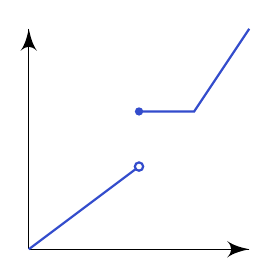
\begin{tikzpicture}[scale=0.7]
      \draw [->] (0, 0) -- (4, 0);
      \draw [->] (0, 0) -- (0, 4);

      \draw [thick, mblue] (0, 0) -- (2, 1.5) node [draw, fill=white, circle, inner sep = 0, minimum size = 3] {};

      \draw [thick, mblue] (2, 2.5) node [circ] {} -- (3, 2.5) -- (4, 4);
    \end{tikzpicture}
  \end{center}
  then $f$ is given by
  \begin{center}
    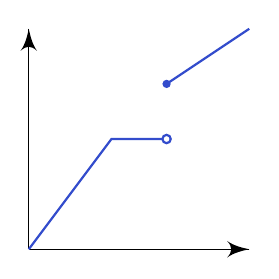
\begin{tikzpicture}[scale=0.7]
      \draw [->] (0, 0) -- (4, 0);
      \draw [->] (0, 0) -- (0, 4);

      \draw [thick, mblue] (0, 0) -- (1.5, 2) -- (2.5, 2) node [draw, fill=white, circle, inner sep = 0, minimum size = 3] {};

      \draw [thick, mblue] (2.5, 3) node [circ] {} -- (4, 4);
    \end{tikzpicture}
  \end{center}
\end{eg}

This allows us to construct new measures on $\R$ with ease.
\begin{thm}
  Let $g: \R \to \R$ be non-constant, non-decreasing and right continuous. Then there exists a unique Radon measure $\d g$ on $\mathcal{B}$ such that
  \[
    \d g((a, b]) = g(b) - g(a).
  \]
  Moreover, we obtain all non-zero Radon measures on $\R$ in this way.
\end{thm}
We have already seen an instance of this when we $g$ was the identity function.

Given the lemma, this is very easy.
\begin{proof}
  Take $I$ and $f$ as in the previous lemma, and let $\mu$ be the restriction of the Lebesgue measure to Borel subsets of $I$. Now $f$ is measurable since it is left continuous. We define $\d g = \mu \circ f^{-1}$. Then we have
  \begin{align*}
    \d g((a, b]) &= \mu(\{x \in I: a < f(x) \leq b\}) \\
    &= \mu(\{x \in I: g(a) < x \leq g(b)\}) \\
    &= \mu((g(a), g(b)]) = g(b) - g(a).
  \end{align*}
  So $\d g$ is a Radon measure with the required property.

  There are no other such measures by the argument used for uniqueness of the Lebesgue measure.

  To show we get all non-zero Radon measures this way, suppose we have a Radon measure $\nu$ on $\R$, we want to produce a $g$ such that $\nu = \d g$. We set
  \[
    g(y) =
    \begin{cases}
      -\nu ((y, 0]) & y \leq 0\\
      \nu((0, y]) & y > 0
    \end{cases}.
  \]
  Then $\nu((a, b]) = g(b) - g(a)$. We see that $\nu$ is non-zero, so $g$ is non-constant. It is also easy to see it is non-decreasing and right continuous. So $\nu = \d g$ by continuity.
\end{proof}

\subsection{Random variables}
We are now going to look at these ideas in the context of probability. It turns out they are concepts we already know and love!

\begin{defi}[Random variable]\index{random variable}
  Let $(\Omega, \mathcal{F}, \P)$ be a probability space, and $(E, \mathcal{E})$ a measurable space. Then an \emph{$E$-valued random variable} is a measurable function $X: \Omega \to E$.

  By default, we will assume the random variables are real.
\end{defi}
Usually, when we have a random variable $X$, we might ask questions like ``what is the probability that $X \in A$?''. In other words, we are asking for the ``size'' of the set of things that get sent to $A$. This is just the image measure!
\begin{defi}[Distribution/law]\index{distribution}
  Given a random variable $X: \Omega \to E$, the \emph{distribution} or \term{law} of $X$ is the image measure $\mu_x: \P \circ X^{-1}$. We usually write
  \[
    \P(X \in A) = \mu_x(A) = \P(X^{-1}(A)).
  \]
\end{defi}
If $E = \R$, then $\mu_x$ is determined by its values on the $\pi$-system of intervals $(-\infty, y]$. We set
\[
  F_X(x) = \mu_X((-\infty, x]) = \P(X \leq x)
\]
This is known as the \term{distribution function}\index{$F_X$} of $X$.

\begin{prop}
  We have
  \[
    F_X(x) \to
    \begin{cases}
      0 & x \to -\infty\\
      1 & x \to +\infty
    \end{cases}.
  \]
  Also, $F_X(x)$ is non-decreasing and right-continuous.
\end{prop}

We call any function $F$ with these properties a distribution function.
\begin{defi}[Distribution function]\index{distribution function}
  A \emph{distribution function} is a non-decreasing, right continuous function $f: \R \to [0, 1]$ satisfying
  \[
    F_X(x) \to
    \begin{cases}
      0 & x \to -\infty\\
      1 & x \to +\infty
    \end{cases}.
  \]
\end{defi}
We now want to show that every distribution function is indeed a distribution.

\begin{prop}
  Let $F$ be any distribution function. Then there exists a probability space $(\Omega, \mathcal{F}, \P)$ and a random variable $X$ such that $F_X = F$.
\end{prop}

\begin{proof}
  Take $(\Omega, \mathcal{F}, \P) = ((0, 1), \mathcal{B}(0, 1), \text{Lebesgue})$. We take $X: \Omega \to \R$ to be
  \[
    X(\omega) = \inf\{x: \omega \leq f(x)\}.
  \]
  Then we have
  \[
    X(\omega) \leq x \Longleftrightarrow w \leq F(x).
  \]
  So we have
  \[
    F_X(x) = \P[X \leq x] = \P[(0, F(x)]] = F(x).
  \]
  Therefore $F_X = F$.
\end{proof}

This construction is actually very useful in practice. If we are writing a computer program and want to sample a random variable, we will use this procedure. The computer usually comes with a uniform (pseudo)-random number generator. Then using this procedure allows us to produce random variables of any distribution from a uniform sample.

The next thing we want to consider is the notion of independence of random variables. Recall that for random variables $X, Y$, we used to say that they are independent if for any $A, B$, we have
\[
  \P[X \in A, Y \in B] = \P[X \in A]\P[Y \in B].
\]
But this is exactly the statement that the $\sigma$-algebras generated by $X$ and $Y$ are independent!

\begin{defi}[Independence of random variables]\index{random variable!independent}\index{independent!random variable}
  A family $(X_n)$ of random variables is said to be \emph{independent} if the family of $\sigma$-algebras $(\sigma(X_n))$ is independent.
\end{defi}

\begin{prop}
  Two real-valued random variables $X, Y$ are independent iff
  \[
    \P[X \leq x, Y \leq y] = \P[X \leq x] \P[Y \leq y].
  \]
  More generally, if $(X_n)$ is a sequence of real-valued random variables, then they are independent iff
  \[
    \P[x_1 \leq x_1, \cdots, x_n \leq x_n] = \prod_{j = 1}^n \P[X_j \leq x_j]
  \]
  for all $n$ and $x_j$.
\end{prop}

\begin{proof}
  The $\Rightarrow$ direction is obvious. For the other direction, we simply note that $\{(-\infty, x]: x \in \R\}$ is a generating $\pi$-system for the Borel $\sigma$-algebra of $\R$.
\end{proof}

In probability, we often say things like ``let $X_1, X_2, \cdots$ be iid random variables''. However, how can we guarantee that iid random variables do indeed exist? We start with the less ambitious goal of finding iid $\Bernoulli(1/2)$ random variables:

\begin{prop}
  Let
  \[
    (\Omega, \mathcal{F}, \P) = ((0, 1), \mathcal{B}(0, 1), \text{Lebesgue}).
  \]
  be our probability space. Then there exists as sequence $R_n$ of independent $\Bernoulli(1/2)$ random variables.
\end{prop}

\begin{proof}
  Suppose we have $\omega \in \Omega = (0, 1)$. Then we write $\omega$ as a binary expansion
  \[
    \omega = \sum_{n = 1}^\infty \omega_n 2^{-n},
  \]
  where $\omega_n \in \{0, 1\}$. We make the binary expansion unique by disallowing infinite sequences of zeroes.

  We define $R_n(\omega) = \omega_n$. We will show that $R_n$ is measurable. Indeed, we can write
  \[
    R_1(\omega) = \omega_1 = \mathbf{1}_{(1/2, 1]}(\omega),
  \]
  where $\mathbf{1}_{(1/2, 1]}$ is the indicator function. Since indicator functions of measurable sets are measurable, we know $R_1$ is measurable. Similarly, we have
  \[
    R_2(\omega) = \mathbf{1}_{(1/4, 1/2]}(\omega) + \mathbf{1}_{(3/4, 1]}(\omega).
  \]
  So this is also a measurable function. More generally, we can do this for any $R_n(\omega)$: we have
  \[
    R_n(\omega) = \sum_{j = 1}^{2^{n - 1}} \mathbf{1}_{(2^{-n}(2j - 1), 2^{-n}(2j)]} (\omega).
  \]
  So each $R_n$ is a random variable, as each can be expressed as a sum of indicators of measurable sets.

  Now let's calculate
  \[
    \P[R_n = 1] = \sum_{j = 1}^{2n - 1} 2^{-n}((2j) - (2j - 1)) = \sum_{j = 1}^{2n - 1} 2^{-n} = \frac{1}{2}.
  \]
  Then we have
  \[
    \P[R_n = 0] = 1 - \P[R_n = 1] = \frac{1}{2}
  \]
  as well. So $R_n \sim \Bernoulli(1/2)$.

  We can straightforwardly check that $(R_n)$ is an independent sequence, since for $n \not= m$, we have
  \[
    \P[R_n = 0 \text{ and }R_m = 0] = \frac{1}{4} = \P[R_n = 0] \P[R_m = 0].
  \]
\end{proof}

We will now use the $(R_n)$ to construct any independent sequence for any distribution.

\begin{prop}
  Let
  \[
    (\Omega, \mathcal{F}, \P) = ((0, 1), \mathcal{B}(0, 1), \text{Lebesgue}).
  \]
  Given any sequence $(F_n)$ of distribution functions, there is a sequence $(X_n)$ of random variables with $F_{X_n} = F_n$ for all $n$.
\end{prop}

\begin{proof}
  Let $m: \N^2 \to \N$ be any bijection, and relabel
  \[
    Y_{k, n} = R_{m(k, n)},
  \]
  where the $R_j$ are as in the previous random variable. We let
  \[
    Y_n = \sum_{k = 1}^\infty 2^{-k} Y_{k, n}.
  \]
  Then we know that $(Y_n)$ is an independent sequence of random variables, and each is uniform on $(0, 1)$. As before, we define
  \[
    G_n(y) = \inf\{x: y \leq F_n(x)\}.
  \]
  We set $X_n = G_n(Y_n)$. Then $(X_n)$ is a sequence of random variables with $F_{X_n} = F_n$.
\end{proof}

We end the section with a random fact: let $(\Omega, \mathcal{F}, \P)$ and $R_j$ be as above. Then $\frac{1}{n} \sum_{j = 1}^n R_j$ is the average of $n$ independent of $\Bernoulli(1/2)$ random variables. The weak law of large numbers says for any $\varepsilon > 0$, we have
\[
  \P\left[\left\lvert\frac{1}{n} \sum_{j = 1}^n R_j - \frac{1}{2}\right\rvert \geq \varepsilon\right] \to 0\text{ as }n\to \infty.
\]
The strong law of large numbers, which we will prove later, says that
\[
  \P\left[\left\{\omega: \frac{1}{n} \sum_{j = 1}^n R_j \to \frac{1}{2}\right\}\right] = 1.
\]
So ``almost every number'' in $(0, 1)$ has an equal proportion of $0$'s and $1$'s in its binary expansion. This is known as the normal number theorem.

\subsection{Convergence of measurable functions}
The next thing to look at is the convergence of measurable functions. In measure theory, wonderful things happen when we talk about convergence. In analysis, most of the time we had to require uniform convergence, or even stronger notions, if we want limits to behave well. However, in measure theory, the kinds of convergence we talk about are somewhat pointwise in nature. In fact, it will be \emph{weaker} than pointwise convergence. Yet, we are still going to get good properties out of them.

\begin{defi}[Convergence almost everywhere]\index{convergence!almost everywhere}\index{almost everywhere}\index{almost sure convergence}\index{convergence!almost sure}
  Suppose that $(E, \mathcal{E}, \mu)$ is a measure space. Suppose that $(f_n), f$ are measurable functions. We say $f_n \to f$ \emph{almost everywhere (a.e.)} if
  \[
    \mu(\{x \in E: f_n(x) \not\to f(x)\}) = 0.
  \]
  If $(E, \mathcal{E}, \mu)$ is a probability space, this is called \emph{almost sure convergence}.
\end{defi}
To see this makes sense, i.e.\ the set in there is actually measurable, note that
\[
  \{x \in E: f_n(x) \not\to f(x)\} = \{x \in E: \limsup |f_n(x) - f(x)| > 0\}.
\]
We have previously seen that $\limsup |f_n - f|$ is non-negative measurable. So the set $\{x \in E: \limsup |f_n(x) - f(x)| > 0\}$ is measurable.

Another useful notion of convergence is convergence in measure.
\begin{defi}[Convergence in measure]\index{convergence!in measure}\index{convergence!in probability}
  Suppose that $(E, \mathcal{E}, \mu)$ is a measure space. Suppose that $(f_n), f$ are measurable functions. We say $f_n \to f$ \emph{in measure} if for each $\varepsilon > 0$, we have
  \[
    \mu(\{x \in E: |f_n(x) - f(x)| \geq \varepsilon\}) \to 0\text{ as } n \to \infty,
  \]
  then we say that $f_n \to f$ \emph{in measure}.

  If $(E, \mathcal{E}, \mu)$ is a probability space, then this is called \emph{convergence in probability}.
\end{defi}
In the case of a probability space, this says
\[
  \P(|X_n - X| \geq \varepsilon) \to 0\text{ as }n \to \infty
\]
for all $\varepsilon$, which is how we state the weak law of large numbers in the past.

After we define integration, we can consider the norms of a function $f$ by
\[
  \|f\|_p = \left(\int |f(x)|^p \;\d x\right)^{1/p}.
\]
Then in particular, if $\|f_n - f\|_p \to 0$, then $f_n \to f$ in measure, and this provides an easy way to see that functions converge in measure.

In general, neither of these notions imply each other. However, the following theorem provides us with a convenient dictionary to translate between the two notions.

\begin{thm}\leavevmode
  \begin{enumerate}
    \item If $\mu(E) < \infty$, then $f_n \to f$ a.e. implies $f_n \to f$ in measure.
    \item For any $E$, if $f_n \to f$ in measure, then there exists a subsequence $(f_{n_k})$ such that $f_{n_k} \to f$ a.e.
  \end{enumerate}
\end{thm}

\begin{proof}\leavevmode
  \begin{enumerate}
    \item First suppose $\mu(E) < \infty$, and fix $\varepsilon > 0$. Consider
      \[
        \mu(\{x \in E: |f_n(x) - f(x)|\leq \varepsilon\}).
      \]
      We use the result from the first example sheet that for any sequence of events $(A_n)$, we have
      \[
        \liminf \mu(A_n) \geq \mu(\liminf A_n).
      \]
      Applying to the above sequence says
      \begin{align*}
        \liminf \mu(\{x: |f_n(x) - f(x)|\leq \varepsilon\}) &\geq \mu(\{x: |f_m (x) - f(x)| \leq \varepsilon\text{ eventually}\})\\
        &\geq \mu(\{x \in E: |f_m(x) - f(x)| \to 0\})\\
        &= \mu(E).
      \end{align*}
      As $\mu(E) < \infty$, we have $\mu(\{x \in E: |f_n(x) - f(x)| > \varepsilon\}) \to 0$ as $n \to \infty$.

    \item Suppose that $f_n \to f$ in measure. We pick a subsequence $(n_k)$ such that
      \[
        \mu\left(\left\{x \in E: |f_{n_k}(x) - f(x)| > \frac{1}{k}\right\}\right) \leq 2^{-k}.
      \]
      Then we have
      \[
        \sum_{k = 1}^\infty \mu\left(\left\{x \in E: f_{n_k}(x) - f(x)|> \frac{1}{k}\right\}\right) \leq \sum_{k = 1}^\infty 2^{-k} = 1 < \infty.
      \]
      By the first Borel--Cantelli lemma, we know
      \[
        \mu\left(\left\{x \in E: |f_{n_k}(x) - f(x)| > \frac{1}{k} \text{ i.o.}\right\}\right) = 0.
      \]
      So $f_{n_k} \to f$ a.e.
  \end{enumerate}
\end{proof}
It is important that we assume that $\mu(E) < \infty$ for the first part.
\begin{eg}
  Consider $(E, \mathcal{E}, \mu) = (\R, \mathcal{B}, \text{Lebesgue})$. Take $f_n(x) = \mathbf{1}_{[n, \infty)}(x)$. Then $f_n(x) \to 0$ for all $x$, and in particular almost everywhere. However, we have
  \[
    \mu\left(\left\{x \in \R: |f_n(x)| > \frac{1}{2}\right\}\right) = \mu([n, \infty)) = \infty
  \]
  for all $n$.
\end{eg}

There is one last type of convergence we are interested in. We will only first formulate it in the probability setting, but there is an analogous notion in measure theory known as \emph{weak convergence}, which we will discuss much later on in the course.
\begin{defi}[Convergence in distribution]\index{convergence!in distribution}
  Let $(X_n), X$ be random variables with distribution functions $F_{X_n}$ and $F_X$, then we say $X_n \to X$ \emph{in distribution} if $F_{X_n}(x) \to F_X(x)$ for all $x \in \R$ at which $F_X$ is continuous.
\end{defi}
Note that here we do not need that $(X_n)$ and $X$ live on the same probability space, since we only talk about the distribution functions.

But why do we have the condition with continuity points? The idea is that if the resulting distribution has a ``jump'' at $x$, it doesn't matter which side of the jump $F_X(x)$ is at. Here is a simple example that tells us why this is very important:

\begin{eg}
  Let $X_n$ to be uniform on $[0, 1/n]$. Intuitively, this should converge to the random variable that is always zero.

  We can compute
  \[
    F_{X_n} (x) =
    \begin{cases}
      0 & x \leq 0\\
      nx & 0 < x< 1/n\\
      1 & x \geq 1/n
    \end{cases}.
  \]
  We can also compute the distribution of the zero random variable as
  \[
    F_0 =
    \begin{cases}
      0 & x < 0\\
      1 & x \geq 0
    \end{cases}.
  \]
  But $F_{X_n}(0) = 0 $ for all $n$, while $F_X(0) = 1$.
\end{eg}
One might now think of cheating by cooking up some random variable such that $F$ is discontinuous at so many points that random, unrelated things converge to $F$. However, this cannot be done, because $F$ is a non-decreasing function, and thus can only have countably many points of discontinuities.

The big theorem we are going to prove about convergence in distribution is that actually it is very boring and doesn't give us anything new.

\begin{thm}[Skorokhod representation theorem of weak convergence]\index{Skorokhod representation theorem of weak convergence}\leavevmode
  \begin{enumerate}
    \item If $(X_n), X$ are defined on the same probability space, and $X_n \to X$ in probability. Then $X_n \to X$ in distribution.
    \item If $X_n \to X$ in distribution, then there exists random variables $(\tilde{X}_n)$ and $\tilde{X}$ defined on a common probability space with $F_{\tilde{X}_n} = F_{X_n}$ and $F_{\tilde{X}} = F_X$ such that $\tilde{X}_n \to \tilde{X}$ a.s.
  \end{enumerate}
\end{thm}

\begin{proof}
  Let $S = \{x \in \R: F_X\text{ is continuous}\}$.
  \begin{enumerate}
    \item Assume that $X_n \to X$ in probability. Fix $x \in S$. We need to show that $F_{X_n}(x) \to F_X(x)$ as $n \to \infty$.

      We fix $\varepsilon > 0$. Since $x \in S$, this implies that there is some $\delta > 0$ such that
      \begin{align*}
        F_X(x - \delta) &\geq F_X(x) - \frac{\varepsilon}{2}\\
        F_X(x + \delta) & \leq F_X(x) + \frac{\varepsilon}{2}.
      \end{align*}
      We fix $N$ large such that $n \geq N$ implies $\P[|X_n - X| \geq \delta] \leq \frac{\varepsilon}{2}$. Then
      \begin{align*}
        F_{X_n}(x) &= \P[X_n \leq x] \\
        &= \P[(X_n - X) + X \leq x] \\
        \intertext{We now notice that $\{(X_n - X) + X \leq x\} \subseteq \{X \leq x + \delta\} \cup \{|X_n - X| > \delta\}$. So we have}
        &\leq \P[X \leq x + \delta] + \P[|X_n - X| > \delta]\\
        &\leq F_X(x + \delta) + \frac{\varepsilon}{2}\\
        &\leq F_X(x) + \varepsilon.
       \end{align*}
       We similarly have
       \begin{align*}
         F_{X_n}(x) &= \P[X_n \leq x] \\
         &\geq \P[X \leq x - \delta] - \P[|X_n - X| > \delta]\\
         &\geq F_X(x - \delta) - \frac{\varepsilon}{2}\\
         &\geq F_X(x) - \varepsilon.
       \end{align*}
       Combining, we have that $n \geq N$ implying $|F_{x_n}(x) - F_X(x)| \leq \varepsilon$. Since $\varepsilon$ was arbitrary, we are done.
     \item Suppose $X_n \to X$ in distribution. We again let
       \[
         (\Omega, \mathcal{F}, \mathcal{B}) = ((0, 1), \mathcal{B}((0, 1)), \text{Lebesgue}).
       \]
       We let
       \begin{align*}
         \tilde{X}_n(\omega) &= \inf\{x : \omega \leq F_{X_n}(x)\},\\
         \tilde{X}(\omega) &= \inf \{x : \omega \leq F_X(x)\}.
       \end{align*}
       Recall from before that $\tilde{X}_n$ has the same distribution function as $X_n$ for all $n$, and $\tilde{X}$ has the same distribution as $X$. Moreover, we have
       \begin{align*}
         \tilde{X}_n(\omega) \leq x &\Leftrightarrow \omega \leq F_{X_n}(x)\\
         x < \tilde{X}_n(\omega) &\Leftrightarrow F_{X_n}(x) < \omega,
       \end{align*}
       and similarly if we replace $X_n$ with $X$.

       We are now going to show that with this particular choice, we have $\tilde{X}_n \to \tilde{X}$ a.s.

       Note that $\tilde{X}$ is a non-decreasing function $(0, 1) \to \R$. Then by general analysis, $\tilde{X}$ has at most countably many discontinuities. We write
       \[
         \Omega_0 = \{\omega \in (0, 1): \tilde{X}\text{ is continuous at }\omega_0\}.
       \]
       Then $(0, 1) \setminus \Omega_0$ is countable, and hence has Lebesgue measure $0$. So
       \[
         \P[\Omega_0] = 1.
       \]
       We are now going to show that $\tilde{X}_n (\omega) \to \tilde{X}(\omega)$ for all $\omega \in \Omega_0$.

       Note that $F_X$ is a non-decreasing function, and hence the points of discontinuity $\R \setminus S$ is also countable. So $S$ is dense in $\R$. Fix $\omega \in \Omega_0$ and $\varepsilon > 0$. We want to show that $|\tilde{X}_n(\omega) - \tilde{X}(\omega)| \leq \varepsilon$ for all $n$ large enough.

       Since $S$ is dense in $\R$, we can find $x^-, x^+$ in $S$ such that
       \[
         x^- < \tilde{X}(\omega) < x^+
       \]
       and $x^+ - x^- < \varepsilon$. What we \emph{want} to do is to use the characteristic property of $\tilde{X}$ and $F_X$ to say that this implies
       \[
         F_X(x^-) < \omega < F_X(x^+).
       \]
       Then since $F_{X_n} \to F_X$ at the points $x^-, x^+$, for sufficiently large $n$, we have
       \[
         F_{X_n}(x^-) < \omega < F_{X_n}(x^+).
       \]
       Hence we have
       \[
         x^- < \tilde{X}_n(\omega) < x^+.
       \]
       Then it follows that $|\tilde{X}_n(\omega) - \tilde{X}(\omega)| < \varepsilon$.

       However, this doesn't work, since $\tilde{X}(\omega) < x^+$ only implies $\omega \leq F_X(x^+)$, and our argument will break down. So we do a funny thing where we introduce a new variable $\omega^+$.

       Since $\tilde{X}$ is continuous at $\omega$, we can find $\omega^+\in (\omega, 1)$ such that $\tilde{X}(\omega^+) \leq x^+$.
       \begin{center}
         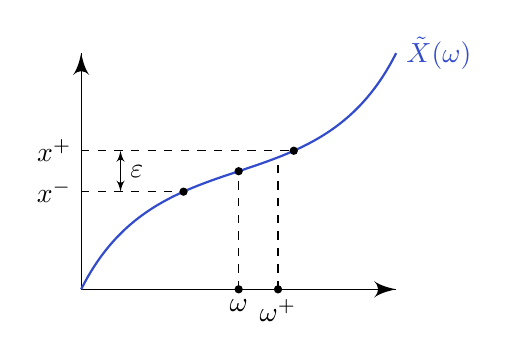
\begin{tikzpicture}
           \draw [->] (0, 0) -- (4, 0);
           \draw [->] (0, 0) -- (0, 3);

           \draw [thick, mblue] (0, 0) .. controls (1, 2) and (3, 1) .. (4, 3) node [right] {$\tilde{X}(\omega)$};

           \node [circ] at (2, 0) {};
           \node [below] at (2, 0) {$\omega$};
           \node [circ] at (2, 1.5) {};

           \draw [dashed] (0, 1.24) node [left] {$x^-$} -- (1.3, 1.24) node [circ] {};
           \draw [dashed] (0, 1.76) node [left] {$x^+$} -- (2.7, 1.76) node [circ] {};

           \node [circ] at (2.5, 0) {};
           \node [below] at (2.5, 0) {$\omega^+$};
           \draw [dashed] (2.5, 0) -- (2.5, 1.63);
           \draw [dashed] (2, 0) -- (2, 1.5);

           \draw [latex'-latex'] (0.5, 1.24) -- (0.5, 1.76) node [pos=0.5, right] {$\varepsilon$};
         \end{tikzpicture}
       \end{center}
       Then we have
       \[
         x^- < \tilde{X}(\omega) \leq \tilde{X}(\omega^+) < x^+.
       \]
       Then we have
       \[
         F_X(x^-) < \omega < \omega^+ \leq F_X(x^+).
       \]
       So for sufficiently large $n$, we have
       \[
         F_{X_n}(x^-) < \omega < F_{X_n}(x^+).
       \]
       So we have
       \[
         x^- < \tilde{X}_n(\omega) \leq x^+,
       \]
       and we are done.
  \end{enumerate}
\end{proof}

\subsection{Tail events}
Finally, we are going to quickly look at tail events. These are events that depend only on the asymptotic behaviour of a sequence of random variables.
\begin{defi}[Tail $\sigma$-algebra]\index{tail $\sigma$-algebra}\index{$\sigma$-algebra!tail}
  Let $(X_n)$ be a sequence of random variables. We let
  \[
    \mathcal{T}_n = \sigma(X_{n + 1}, X_{n + 2}, \cdots),
  \]
  and
  \[
    \mathcal{T} = \bigcap_n \mathcal{T}_n.
  \]
  Then $\mathcal{T}$ is the \emph{tail $\sigma$-algebra}.
\end{defi}
Then $\mathcal{T}$-measurable \index{$\mathcal{T}$-measurable} events and random variables only depend on the asymptotic behaviour of the $X_n$'s.

\begin{eg}
  Let $(X_n)$ be a sequence of real-valued random variables. Then
  \[
    \limsup_{n \to \infty} \frac{1}{n} \sum_{j = 1}^n X_j,\quad \liminf_{n \to \infty} \frac{1}{n} \sum_{j = 1}^n X_j
  \]
  are $\mathcal{T}$-measurable random variables. Finally,
  \[
    \left\{\lim_{n \to \infty} \frac{1}{n} \sum_{j = 1}^n X_j\text{ exists }\right\} \in \mathcal{T},
  \]
  since this is just the set of all points where the previous two things agree.
\end{eg}

\begin{thm}[Kolmogorov 0-1 law]\index{Kolmogorov 0-1 law}
  Let $(X_n)$ be a sequence of independent (real-valued) random variables. If $A \in \mathcal{T}$, then $\P[A] = 0$ or $1$.

  Moreover, if $X$ is a $\mathcal{T}$-measurable random variable, then there exists a constant $c$ such that
  \[
    \P[X = c] = 1.
  \]
\end{thm}

\begin{proof}
  The proof is very funny the first time we see it. We are going to prove the theorem by checking something that seems very strange. We are going to show that if $A \in \mathcal{T}$, then $A$ is independent of $A$. It then follows that
  \[
    \P[A] = \P[A \cap A] = \P[A] \P[A],
  \]
  so $\P[A] = 0$ or $1$. In fact, we are going to prove that $\mathcal{T}$ is independent of $\mathcal{T}$.

  Let
  \[
    \mathcal{F}_n = \sigma(X_1, \cdots, X_n).
  \]
  This $\sigma$-algebra is generated by the $\pi$-system of events of the form
  \[
    A = \{X_1 \leq x_1, \cdots, X_n \leq x_n\}.
  \]
  Similarly, $\mathcal{T}_n = \sigma(X_{n + 1}, X_{n + 2}, \cdots)$ is generated by the $\pi$-system of events of the form
  \[
    B = \{X_{n + 1} \leq x_{n + 1}, \cdots, X_{n + k} \leq x_{n + k}\},
  \]
  where $k$ is any natural number.

  Since the $X_n$ are independent, we know for any such $A$ and $B$, we have
  \[
    \P[A \cap B] = \P[A]\P[B].
  \]
  Since this is true for all $A$ and $B$, it follows that $\mathcal{F}_n$ is independent of $\mathcal{T}_n$.

  Since $\mathcal{T} = \bigcap_k \mathcal{T}_k \subseteq \mathcal{T}_n$ for each $n$, we know $\mathcal{F}_n$ is independent of $\mathcal{T}$.

  Now $\bigcup_k \mathcal{F}_k$ is a $\pi$-system, which generates the $\sigma$-algebra $\mathcal{F}_\infty = \sigma(X_1, X_2, \cdots)$. We know that if $A \in \bigcup_n \mathcal{F}_n$, then there has to exist an index $n$ such that $A \in \mathcal{F}_n$. So $A$ is independent of $\mathcal{T}$. So $\mathcal{F}_\infty$ is independent of $\mathcal{T}$.

  Finally, note that $\mathcal{T} \subseteq \mathcal{F}_\infty$. So $\mathcal{T}$ is independent of $\mathcal{T}$.

  To find the constant, suppose that $X$ is $\mathcal{T}$-measurable. Then
  \[
    \P[X \leq x] \in \{0, 1\}
  \]
  for all $x \in \R$ since $\{X \leq x\} \in \mathcal{T}$.

  Now take
  \[
    c = \inf\{x \in \R: \P[X \leq x] = 1\}.
  \]
  Then with this particular choice of $c$, it is easy to see that $\P[X = c] = 1$. This completes the proof of the theorem.
\end{proof}

\section{Integration}
\subsection{Definition and basic properties}
We are now going to work towards defining the integral of a measurable function on a measure space $(E, \mathcal{E}, \mu)$. Different sources use different notations for the integral. The following notations are all commonly used:
\[
  \mu(f) = \int_E f \;\d \mu = \int_E f(x) \;\d \mu(x) = \int_E f(x) \mu(\d x).
\]
In the case where $(E, \mathcal{E}, \mu) = (\R, \mathcal{B}, \mathrm{Lebesgue})$, people often just write this as
\[
  \mu(f) = \int_\R f(x)\;\d x.
\]
On the other hand, if $(E, \mathcal{E}, \mu) = (\Omega, \F, \P)$ is a probability space, and $X$ is a random variable, then people write the integral as $\E[X]$, the \term{expectation} of $X$.\index{$\E[X]$}\index{$\mu(f)$}

So how are we going to define the integral? There are two steps to defining the integral. The idea is that we first define the integral on \emph{simple functions}, and then extend the definition to more general measurable functions by taking the limit. When we do the definition for simple functions, it will be obvious that the definition satisfies the nice properties, and we will have to check that they are preserved when we take the limit.

\begin{defi}[Simple function]\index{simple function}
  A \emph{simple function} is a measurable function that can be written as a finite non-negative linear combination of indicator functions of measurable sets, i.e.
  \[
    f = \sum_{k = 1}^n a_k \mathbf{1}_{A_k}
  \]
  for some $A_k \in \mathcal{E}$ and $a_k \geq 0$.
\end{defi}
Note that some sources do not assume that $a_k \geq 0$, but assuming this makes our life easier.

It is obvious that
\begin{prop}
  A function is simple iff it is measurable, non-negative, and takes on only finitely-many values.
\end{prop}

\begin{defi}[Integral of simple function]\index{integral!simple function}\index{simple function!integral}
  The integral of a simple function
  \[
    f = \sum_{k = 1}^n a_k \mathbf{1}_{A_k}
  \]
  is given by
  \[
    \mu(f) = \sum_{k = 1}^n a_k \mu(A_k).
  \]
\end{defi}
Note that it can be that $\mu(A_k) = \infty$, but $a_k = 0$. When this happens, we are just going to declare that $0 \cdot \infty = 0$ (this makes sense because this means we are ignoring all $0 \cdot\mathbf{1}_A$ terms for any $A$). After we do this, we can check the integral is well-defined.

We are now going to extend this definition to non-negative measurable functions by a limiting procedure. Once we've done this, we are going to extend the definition to measurable functions by linearity of the integral. Then we would have a definition of the integral, and we are going to deduce properties of the integral using approximation.

\begin{defi}[Integral]\index{integral}
  Let $f$ be a non-negative measurable function. We set
  \[
    \mu(f) = \sup\{\mu(g): g \leq f, g\text{ is simple}\}.
  \]
  For arbitrary $f$, we write
  \[
    f = f^+ - f^- = (f \vee 0) + (f \wedge 0).
  \]
  We put $|f| = f^+ + f^-$. We say $f$ is \emph{integrable}\index{integrable function} if $\mu(|f|) < \infty$. In this case, set
  \[
    \mu(f) = \mu(f^+) - \mu(f^-).
  \]
  If only one of $\mu(f^+), \mu(f_-) < \infty$, then we can still make the above definition, and the result will be infinite.
\end{defi}

In the case where we are integrating over (a subset of) the reals, we call it the \term{Lebesgue integral}.

\begin{prop}
  Let $f: [0, 1] \to \R$ be Riemann integrable. Then it is also Lebesgue integrable, and the two integrals agree.
\end{prop}
We will not prove this, but this immediately gives us results like the fundamental theorem of calculus, and also helps us to actually compute the integral. However, note that this does not hold for infinite domains, as you will see in the second example sheet.

But the Lebesgue integrable functions are better. A lot of functions are Lebesgue integrable but not Riemann integrable.
\begin{eg}
  Take the standard non-Riemann integrable function
  \[
    f = \mathbf{1}_{[0, 1]\setminus \Q}.
  \]
  Then $f$ is not Riemann integrable, but it is Lebesgue integrable, since
  \[
    \mu(f) = \mu([0, 1] \setminus \Q) = 1.
  \]
\end{eg}

We are now going to study some basic properties of the integral. We will first look at the properties of integrals of simple functions, and then extend them to general integrable functions.

For $f, g$ simple, and $\alpha, \beta \geq 0$, we have that
\[
  \mu(\alpha f + \beta g) = \alpha \mu(f) + \beta\mu(g).
\]
So the integral is linear.

Another important property is monotonicity --- if $f \leq g$, then $\mu(f) \leq \mu(g)$.

Finally, we have $f = 0$ a.e. iff $\mu(f) = 0$. It is absolutely crucial here that we are talking about non-negative functions.

Our goal is to show that these three properties are also satisfied for arbitrary non-negative measurable functions, and the first two hold for integrable functions.

In order to achieve this, we prove a very important tool --- the monotone convergence theorem. Later, we will also learn about the dominated convergence theorem and Fatou's lemma. These are the main and very important results about exchanging limits and integration.

\begin{thm}[Monotone convergence theorem]\index{monotone convergence theorem}
  Suppose that $(f_n), f$ are non-negative measurable with $f_n \nearrow f$. Then $\mu(f_n) \nearrow \mu(f)$.
\end{thm}

In the proof we will use the fact that the integral is monotonic, which we shall prove later.
\begin{proof}
  We will split the proof into five steps. We will prove each of the following in turn:
  \begin{enumerate}
    \item If $f_n$ and $f$ are indicator functions, then the theorem holds.
    \item If $f$ is an indicator function, then the theorem holds.
    \item If $f$ are simple, then the theorem holds.
    \item If $f$ is non-negative measurable, then the theorem holds.
  \end{enumerate}
  Each part follows rather straightforwardly from the previous one, and the reader is encouraged to try to prove it themself.

  \separator

  We first consider the case where $f_n = \mathbf{1}_{A_n}$ and $f = \mathbf{1}_A$. Then $f_n \nearrow f$ is true iff $A_n \nearrow A$. On the other hand, $\mu(f_n) \nearrow \mu(f)$ iff $\mu(A_n) \nearrow \mu(A)$.

  For convenience, we let $A_0 = \emptyset$. We can write
  \begin{align*}
    \mu(A) &= \mu\left(\bigcup_n A_n \setminus A_{n - 1}\right) \\
    &= \sum_{n = 1}^\infty \mu(A_n \setminus A_{n - 1}) \\
    &= \lim_{N \to \infty} \sum_{n = 1}^N \mu(A_n \setminus A_{n - 1}) \\
    &= \lim_{N \to \infty}\mu (A_N).
  \end{align*}
  So done.

  \separator

  We next consider the case where $f = \mathbf{1}_A$ for some $A$. Fix $\varepsilon > 0$, and set
  \[
    A_n = \{f_n > 1 - \varepsilon\} \in \mathcal{E}.
  \]
  Then we know that $A_n \nearrow A$, as $f_n \nearrow f$. Moreover, by definition, we have
  \[
    (1 - \varepsilon) \mathbf{1}_{A_n} \leq f_n \leq f = \mathbf{1}_A.
  \]
  As $A_n \nearrow A$, we have that
  \[
    (1 - \varepsilon) \mu(f) = (1 - \varepsilon) \lim_{n \to \infty} \mu(A_n) \leq \lim_{n \to \infty} \mu(f_n) \leq \mu(f)
  \]
  since $f_n \leq f$. Since $\varepsilon$ is arbitrary, we know that
  \[
    \lim_{n \to \infty} \mu(f_n) = \mu(f).
  \]

  \separator

  Next, we consider the case where $f$ is both simple. We write
  \[
    f = \sum_{k = 1}^m a_k \mathbf{1}_{A_k},
  \]
  where $a_k > 0$ and $A_k$ are pairwise disjoint. Since $f_n \nearrow f$, we know
  \[
    a_k^{-1} f_n \mathbf{1}_{A_k} \nearrow \mathbf{1}_{A_k}.
  \]
  So we have
  \[
    \mu(f_n) = \sum_{k = 1}^m \mu(f_n \mathbf{1}_{A_k}) = \sum_{k = 1}^m a_k \mu(a_k^{-1} f_n \mathbf{1}_{A_k}) \to \sum_{k = 1}^m a_k \mu(A_k) = \mu(f).
  \]

  \separator

  Suppose $f$ is non-negative measurable. Suppose $g \leq f$ is a simple function. As $f_n \nearrow f$, we know $f_n \wedge g \nearrow f \wedge g = g$. So by the previous case, we know that
  \[
    \mu(f_n \wedge g) \to \mu(g).
  \]
  We also know that
  \[
    \mu(f_n) \geq \mu(f_n\wedge g).
  \]
  So we have
  \[
    \lim_{n \to \infty} \mu(f_n) \geq \mu(g)
  \]
  for all $g \leq f$. This is possible only if
  \[
    \lim_{n \to \infty} \mu(f_n) \geq \mu(f)
  \]
  by definition of the integral. However, we also know that $\mu(f_n) \leq \mu(f)$ for all $n$, again by definition of the integral. So we must have equality. So we have
  \[
    \mu(f) = \lim_{n \to \infty} \mu(f_n).
  \]
\end{proof}

\begin{thm}
  Let $f, g$ be non-negative measurable, and $\alpha, \beta \geq 0$. We have that
  \begin{enumerate}
    \item $\mu(\alpha f + \beta g) = \alpha \mu(f) + \beta \mu(g)$.
    \item $f \leq g$ implies $\mu(f) \leq \mu(g)$.
    \item $f = 0$ a.e. iff $\mu(f) = 0$.
  \end{enumerate}
\end{thm}

\begin{proof}\leavevmode
  \begin{enumerate}
    \item Let
      \begin{align*}
        f_n = 2^{-n}\lfloor 2^n f\rfloor \wedge n\\
        g_n = 2^{-n}\lfloor 2^n g\rfloor \wedge n.
      \end{align*}
      Then $f_n, g_n$ are simple with $f_n \nearrow f$ and $g_n \nearrow g$. Hence $\mu(f_n) \nearrow \mu(f)$ and $\mu(g_n \nearrow g$ and $\mu(\alpha f_n + \beta g_n) \nearrow \mu(\alpha f + \beta g)$, by the monotone convergence theorem. As $f_n, g_n$ are simple, we have that
      \[
        \mu(\alpha f_n + \beta g_n) = \alpha \mu(f_n) + \beta \mu(g_n).
      \]
      Taking the limit as $n \to \infty$, we get
      \[
        \mu(\alpha f + \beta g) = \alpha \mu(f) + \beta \mu(g).
      \]
    \item We shall be careful not to use the monotone convergence theorem. We have
      \begin{align*}
        \mu(g) &= \sup\{\mu(h): h \leq g\text{ simple}\}\\
        &\geq \sup \{\mu(h): h \leq f\text{ simple}\}\\
        &= \mu(f).
      \end{align*}
    \item Suppose $f \not= 0$ a.e. Let
      \[
        A_n = \left\{x: f(x) > \frac{1}{n}\right\}.
      \]
      Then
      \[
        \{x: f(x) \not= 0\} = \bigcup_n A_n.
      \]
      Since the left hand set has non-negative measure, it follows that there is some $A_n$ with non-negative measure. For that $n$, we define
      \[
        h = \frac{1}{n} \mathbf{1}_{A_n}.
      \]
      Then $\mu(f) \geq \mu(h) > 0$. So $\mu(f) \not= 0$.

      Conversely, suppose $f = 0$ a.e. We let
      \[
        f_n = 2^{-n} \lfloor 2^n f\rfloor \wedge n
      \]
      be a simple function. Then $f_n \nearrow f$ and $f_n = 0$ a.e. So
      \[
        \mu(f) = \lim_{n \to \infty}\mu(f_n) = 0.
      \]
  \end{enumerate}
\end{proof}

We now prove the analogous statement for general integrable functions.
\begin{thm}
  Let $f, g$ be integrable, and $\alpha, \beta \geq 0$. We have that
  \begin{enumerate}
    \item $\mu(\alpha f + \beta g) = \alpha \mu(f) + \beta \mu(g)$.
    \item $f \leq g$ implies $\mu(f) \leq \mu(g)$.
    \item $f = 0$ a.e. implies $\mu(f) = 0$.
  \end{enumerate}
\end{thm}
Note that in the last case, the converse is no longer true, as one can easily see from the sign function $\sgn: [-1, 1] \to \R$.

\begin{proof}\leavevmode
  \begin{enumerate}
    \item We are going to prove these by applying the previous theorem.

      By definition of the integral, we have $\mu(-f) = - \mu(f)$. Also, if $\alpha \geq 0$, then
      \[
        \mu(\alpha f) = \mu(\alpha f^+) - \mu(\alpha f^-) = \alpha \mu(f^+) - \alpha \mu(f^-) = \alpha \mu(f).
      \]
      Combining these two properties, it then follows that if $\alpha$ is a real number, then
      \[
        \mu(\alpha f) = \alpha \mu(f).
      \]
      To finish the proof of (i), we have to show that $\mu(f + g) = \mu(f) + \mu(g)$. We know that this is true for non-negative functions, so we need to employ a little trick to make this a statement about the non-negative version. If we let $h = f + g$, then we can write this as
      \[
        h^+ - h^- = (f^+ - f^-) + (g^+ - g^-).
      \]
      We now rearrange this as
      \[
        h^ + f^- + g^- = f^+ + g^+ + h^-.
      \]
      Now everything is non-negative measurable. So applying $\mu$ gives
      \[
        \mu(f^+) + \mu(f^-) + \mu(g^-) = \mu(f^+) + \mu(g^+) + \mu(h^-).
      \]
      Rearranging, we obtain
      \[
        \mu(h^+) - \mu (h^-) = \mu(f^+) - \mu(f^-) + \mu(g^+) - \mu(g^-).
      \]
      This is exactly the same thing as saying
      \[
        \mu(f + g) = \mu(h) = \mu(f) = \mu(g).
      \]
    \item If $f \leq g$, then $g - f \geq 0$. So $\mu(g - f) \geq 0$. By (i), we know $\mu(g) - \mu(f) \geq 0$. So $\mu(g) \geq \mu(f)$.

    \item If $f = 0$ a.e., then $f^+, f^- = 0$ a.e. So $\mu(f^+) = \mu(f^-) = 0$. So $\mu(f) = \mu(f^+) - \mu(f^-) = 0$.
  \end{enumerate}
\end{proof}
As mentioned, the converse to (iii) is no longer true. However, we do have the following partial converse:
\begin{prop}
  If $\mathcal{A}$ is a $\pi$-system with $E \in \mathcal{A}$ and $\sigma(\mathcal{A}) = \mathcal{E}$, and $f$ is an integrable function that
  \[
    \mu(f\mathbf{1}_A) =0
  \]
  for all $A \in \mathcal{A}$. Then $\mu(f) = 0$ a.e.
\end{prop}

\begin{proof}
  Let
  \[
    \mathcal{D} = \{A \in \mathcal{E}: \mu (f\mathbf{1}_A) = 0\}.
  \]
  It follows immediately from the properties of the integral that $\mathcal{D}$ is a d-system. So $\mathcal{D} = \mathcal{E}$ by Dynkin's lemma. Let
  \begin{align*}
    A^+ &= \{x \in E: f(x) > 0\},\\
    A^- &= \{x \in E: f(x) < 0\}.
  \end{align*}
  Then $A^{\pm} \in \mathcal{E}$, and
  \[
    \mu(f \mathbf{1}_{A^+}) = \mu(f \mathbf{1}_{A^-}) = 0.
  \]
  So $f\mathbf{1}_{A^+}$ and $f \mathbf{1}_{A^-}$ vanish a.e. So $f$ vanishes a.e.
\end{proof}

\begin{prop}
  Suppose that $(g_n)$ is a sequence of non-negative measurable functions. Then we have
  \[
    \mu\left(\sum_{n = 1}^\infty g_n\right) = \sum_{n = 1}^\infty \mu(g_n).
  \]
\end{prop}

\begin{proof}
  We know
  \[
    \left(\sum_{n = 1}^N g_n\right) \nearrow \left(\sum_{n = 1}^\infty g_n\right)
  \]
  as $N \to \infty$. So by the monotone convergence theorem, we have
  \[
    \sum_{n = 1}^N \mu(g_n) = \mu \left(\sum_{n = 1}^N g_n\right) \nearrow \mu\left(\sum_{n = 1}^\infty g_n\right).
  \]
  But we also know that
  \[
    \sum_{n = 1}^N \mu(g_n) \nearrow \sum_{n = 1}^\infty \mu(g_n)
  \]
  by definition. So we are done.
\end{proof}

So for non-negative measurable functions, we can always switch the order of integration and summation.

Note that we can consider summation as integration. We let $E = \N$ and $\mathcal{E} = \{\text{all subsets of $\N$}\}$. We let $\mu$ be the counting measure, so that $\mu(A)$ is the size of $A$. Then integrability (and having a finite integral) is the same as absolute convergence. Then if it converges, then we have
\[
  \int f \;\d \mu = \sum_{n = 1}^\infty f(n).
\]
So we can just view our proposition as proving that we can swap the order of two integrals. The general statement is known as Fubini's theorem.

\subsection{Integrals and limits}
We are now going to prove more things about exchanging limits and integrals. These are going to be extremely useful in the future, as we want to exchange limits and integrals a lot.

\begin{thm}[Fatou's lemma]\index{Fatou's lemma}
  Let $(f_n)$ be a sequence of non-negative measurable functions. Then
  \[
    \mu(\lim\inf f_n) \leq \lim\inf \mu(f_n).
  \]
\end{thm}
Note that a special case was proven in the first example sheet, where we did it for the case where $f_n$ are indicator functions.

\begin{proof}
  We start with the trivial observation that if $k\geq n$, then we always have that
  \[
    \inf_{m \geq n} f_m \leq f_k.
  \]
  By the monotonicity of the integral, we know that
  \[
    \mu\left(\inf_{m \geq n} f_m\right) \leq \mu(f_k).
  \]
  for all $k \geq n$.

  So we have
  \[
    \mu\left(\inf_{m \geq n} f_m\right) \leq \inf_{k \geq n} \mu(f_k) \leq \liminf_m \mu(f_m).
  \]
  It remains to show that the left hand side converges to $\mu(\liminf f_m)$. Indeed, we know that
  \[
    \inf_{m \geq n} f_m \nearrow \liminf_m f_m.
  \]
  Then by monotone convergence, we have
  \[
    \mu\left(\inf_{m \geq n} f_m\right) \nearrow \mu\left(\liminf_m f_m\right).
  \]
  So we have
  \[
    \mu\left(\liminf_m f_m\right) \leq \liminf_m \mu(f_m).
  \]
\end{proof}
No one ever remembers which direction Fatou's lemma goes, and this leads to many incorrect proofs and results, so it is helpful to keep the following example in mind:

\begin{eg}
  We let $(E, \mathcal{E}, \mu) = (\R, \mathcal{B}, \text{Lebesgue})$. We let
  \[
    f_n = \mathbf{1}_{[n, n + 1]}.
  \]
  Then we have
  \[
    \liminf_n f_n = 0.
  \]
  So we have
  \[
    \mu(f_n) = 1\text{ for all }n.
  \]
  So we have
  \[
    \liminf \mu(f_n) = 1,\quad \mu(\liminf f_n) = 0.
  \]
  So we have
  \[
    \mu\left(\liminf_m f_m\right) \leq \liminf_m \mu(f_m).
  \]
\end{eg}
The next result we want to prove is the dominated convergence theorem. This is like the monotone convergence theorem, but we are going to remove the increasing and non-negative measurable condition, and add in something else.
\begin{thm}[Dominated convergence theorem]\index{dominated convergence theorem}
  Let $(f_n), f$ be measurable with $f_n(x) \to f(x)$ for all $x \in E$. Suppose that there is an integrable function $g$ such that
  \[
    |f_n| \leq g
  \]
  for all $n$, then we have
  \[
    \mu(f_n) \to \mu(f)
  \]
  as $n \to \infty$.
\end{thm}

\begin{proof}
  Note that
  \[
    |f| = \lim_n |f|_n \leq g.
  \]
  So we know that
  \[
    \mu(|f|) \leq \mu(g) < \infty.
  \]
  So we know that $f$, $f_n$ are integrable.

  Now note also that
  \[
    0 \leq g + f_n,\quad 0 \leq g - f_n
  \]
  for all $n$. We are now going to apply Fatou's lemma twice with these series. We have that
  \begin{align*}
    \mu(g) + \mu(f) &= \mu(g + f) \\
    &= \mu\left(\liminf_n (g + f_n)\right) \\
    &\leq \liminf_n \mu(g + f_n)\\
    &= \liminf_n (\mu(g) + \mu(f_n))\\
    &= \mu(g) + \liminf_n \mu(f_n).
  \end{align*}
  Since $\mu(g)$ is finite, we know that
  \[
    \mu(f) \leq \liminf_n \mu(f_n).
  \]
  We now do the same thing with $g - f_n$. We have
  \begin{align*}
    \mu(g) - \mu(f) &= \mu(g - f) \\
    &= \mu\left(\liminf_n (g - f_n)\right) \\
    &\leq \liminf_n \mu(g - f_n)\\
    &= \liminf_n (\mu(g) - \mu(f_n))\\
    &= \mu(g) - \limsup_n \mu(f_n).
  \end{align*}
  Again, since $\mu(g)$ is finite, we know that
  \[
    \mu(f) \geq \limsup_n \mu(f_n).
  \]
  These combine to tell us that
  \[
    \mu(f) \leq \liminf_n \mu(f_n) \leq \limsup_n \mu(f_n) \leq \mu(f).
  \]
  So they must be all equal, and thus $\mu(f_n) \to \mu(f)$.
\end{proof}

\subsection{New measures from old}
We have previously considered several ways of constructing measures from old ones, such as the image measure. We are now going to study a few more ways of constructing new measures, and see how integrals behave when we do these.

\begin{defi}[Restriction of measure space]\index{restriction of measure space}\index{measure space!restriction}
  Let $(E, \mathcal{E}, \mu)$ be a measure space, and let $A \in \mathcal{E}$. The \emph{restriction} of the measure space to $A$ is $(A, \mathcal{E}_A, \mu_A)$, where
  \[
    \mathcal{E}_A = \{B \in \mathcal{E}: B \subseteq A\},
  \]
  and $\mu_A$ is the restriction of $\mu$ to $\mathcal{E}_A$, i.e.
  \[
    \mu_A(B) = \mu(B)
  \]
  for all $B \in \mathcal{E}_A$.
\end{defi}

It is easy to check the following:
\begin{lemma}
  For $(E, \mathcal{E}, \mu)$ a measure space and $A \in \mathcal{E}$, the restriction to $A$ is a measure space.
\end{lemma}

%\begin{proof}
% We check that $\mathcal{E}_A$ is a $\sigma$-algebra.
%
% Since $\emptyset \in \mathcal{E}$ and $\emptyset\subseteq A$, we know $\phi \in \mathcal{E}_A$.
%
% Also, if $B \in \mathcal{E}$ and $B \subseteq A$, then $A \cap B^C \in \mathcal{E}$. So $A \setminus B \in \mathcal{E}_A$.
%
% Finally, if $B_n$ is a sequence in $\mathcal{E}$ and $B_n \subseteq A$ for all $n$, then $\bigcup_n B_n \in \mathcal{E}$ and $\bigcup_n B_n \subseteq A$. So $\bigcup_n B_n \in \mathcal{E}_A$.
%
% It is clear that $\mu_A$ is also a measure.
%\end{proof}

\begin{prop}
  Let $(E, \mathcal{E}, \mu)$ and $(F, \mathcal{F}, \mu')$ be measure spaces and $A \in \mathcal{E}$. Let $f: E \to F$ be a measurable function. Then $f|_A$ is $\mathcal{E}_A$-measurable.
\end{prop}

\begin{proof}
  Let $B \in \mathcal{F}$. Then
  \[
    (f|_A)^{-1}(B) = f^{-1}(B) \cap A \in \mathcal{E}_A.
  \]
\end{proof}

Similarly, we have
\begin{prop}
  If $f$ is integrable, then $f|_A$ is $\mu_A$-integrable and $\mu_A(f|_A) = \mu (f\mathbf{1}_A)$.
\end{prop}

Note that means we have
\[
  \mu(f\mathbf{1}_A) = \int_E f\mathbf{1}_A \;\d \mu = \int_A f \;\d \mu_A.
\]
Usually, we are lazy and just write
\[
  \mu(f\mathbf{1}_A) = \int_A f\;\d \mu.
\]
In the particular case of Lebesgue integration, if $A$ is an interval with left and right end points $a, b$ (i.e.\ it can be open, closed, half open or half closed), then we write
\[
  \int_A f\;\d \mu = \int_a^b f(x) \;\d x.
\]
There is another construction we would be interested in.
\begin{defi}[Pushforward/image of measure]\index{pushforward of measure}\index{image measure}\index{measure!pushforward}\index{measure!image}
  Let $(E, \mathcal{E})$ and $(G, \mathcal{G})$ be measure spaces, and $f: E \to G$ a measurable function. If $\mu$ is a measure on $(E, \mathcal{E})$, then
  \[
    \nu = \mu \circ f^{-1}
  \]
  is a measure on $(G, \mathcal{G})$, known as the \emph{pushforward} or \emph{image} measure.
\end{defi}
We have already seen this before, but we can apply this to integration as follows:

\begin{prop}
  If $g$ is a non-negative measurable function on $G$, then
  \[
    \nu(g) = \mu(g \circ f).
  \]
\end{prop}

\begin{proof}
  Exercise using the monotone class theorem (see example sheet).
\end{proof}

Finally, we can specify a measure by \emph{specifying a density}.
\begin{defi}[Density]\index{density}
  Let $(E, \mathcal{E}, \mu)$ be a measure space, and $f$ be a non-negative measurable function. We define
  \[
    \nu(A) = \mu(f \mathbf{1}_A)
  .\]
  Then $\nu$ is a measure on $(E, \mathcal{E})$.
\end{defi}

\begin{prop}
  The $\nu$ defined above is indeed a measure.
\end{prop}

\begin{proof}\leavevmode
  \begin{enumerate}
    \item $\nu(\phi) = \mu(f\mathbf{1}_\emptyset) = \mu(0) = 0$.
    \item If $(A_n)$ is a disjoint sequence in $\mathcal{E}$, then
      \[
        \nu\left(\bigcup A_n\right) = \mu(f\mathbf{1}_{\bigcup A_n}) = \mu\left(f \sum\mathbf{1}_{A_n}\right) = \sum \mu\left(f \mathbf{1}_{A_n}\right) = \sum \nu(f).
      \]
  \end{enumerate}
\end{proof}

\begin{defi}[Density]\index{density!random variable}\index{random variable!density}
  Let $X$ be a random variable. We say $X$ has a density if its law $\mu_X$ has a density with respect to the Lebesgue measure. In other words, there exists $f_X$ non-negative measurable so that
  \[
    \mu_X(A) = \P[X \in A] = \int_A f_X(x)\;\d x.
  \]
  In this case, for any non-negative measurable function, for any non-negative measurable $g$, we have that
  \[
    \E[g(X)] = \int_\R g(x) f_X(x) \;\d x.
  \]
\end{defi}

\subsection{Integration and differentiation}
In ``normal'' calculus, we had three results involving both integration and differentiation. One was the fundamental theorem of calculus, which we already stated. The others are the change of variables formula, and differentiating under the integral sign.

We start by proving the change of variables formula.
\begin{prop}[Change of variables formula]\index{change of variables formula}
  Let $\phi: [a, b] \to \R$ be continuously differentiable and increasing. Then for any bounded Borel function $g$, we have
  \[
    \int_{\phi(a)}^{\phi(b)} g(y) \;\d y = \int_a^b g(\phi(x))\phi'(x)\;\d x.\tag{$*$}
  \]
\end{prop}

We will use the monotone class theorem.
\begin{proof}
  We let
  \[
    V = \{\text{Borel functions $g$ such that $(*)$ holds}\}.
  \]
  We will want to use the monotone class theorem to show that this includes all bounded functions.

  We already know that
  \begin{enumerate}
    \item $V$ contains $\mathbf{1}_A$ for all $A$ in the $\pi$-system of intervals of the form $[u, v] \subseteq [a, b]$. This is just the fundamental theorem of calculus.
    \item By linearity of the integral, $V$ is indeed a vector space.
    \item Finally, let $(g_n)$ be a sequence in $V$, and $g_n \geq 0$, $g_n \nearrow g$. Then we know that
      \[
        \int_{\phi(a)}^{\phi(b)} g_n(y) \;\d y = \int_a^b g_n(\phi(x))\phi'(x)\;\d x.
      \]
      By the monotone convergence theorem, these converge to
      \[
        \int_{\phi(a)}^{\phi(b)} g(y) \;\d y = \int_a^b g(\phi(x))\phi'(x) \;\d x.
      \]
  \end{enumerate}
  Then by the monotone class theorem, $V$ contains all bounded Borel functions.
\end{proof}

The next problem is differentiation under the integral sign. We want to know when we can say
\[
  \frac{\d}{\d t} \int f(x, t) \;\d x = \int \frac{\partial f}{\partial t}(x, t) \;\d x.
\]

\begin{thm}[Differentiation under the integral sign]\index{differentiation under the integral sign}
  Let $(E, \mathcal{E}, \mu)$ be a space, and $U \subseteq \R$ be an open set, and $f: U \times E \to \R$. We assume that
  \begin{enumerate}
    \item For any $t \in U$ fixed, the map $x \mapsto f(t, x)$ is integrable;
    \item For any $x \in E$ fixed, the map $t \mapsto f(t, x)$ is differentiable;
    \item There exists an integrable function $g$ such that
      \[
        \left|\frac{\partial f}{\partial t}(t, x)\right| \leq g(x)
      \]
      for all $x \in E$ and $t \in U$.
  \end{enumerate}
  Then the map
  \[
    x \mapsto \frac{\partial f}{\partial t}(t, x)
  \]
  is integrable for all $t$, and also the function
  \[
    F(t) = \int_E f(t, x) \d \mu
  \]
  is differentiable, and
  \[
    F'(t) = \int_E \frac{\partial f}{\partial t}(t, x)\;\d \mu.
  \]
\end{thm}
The reason why we want the derivative to be bounded is that we want to apply the dominated convergence theorem.

\begin{proof}
  Measurability of the derivative follows from the fact that it is a limit of measurable functions, and then integrability follows since it is bounded by $g$.

  Suppose $(h_n)$ is a positive sequence with $h_n \to 0$. Then let
  \[
    g_n(x) = \frac{f(t + h_n, x) - f(t, x)}{h_n} - \frac{\partial f}{\partial t}(t, x).
  \]
  Since $f$ is differentiable, we know that $g_n(x) \to 0$ as $n \to \infty$. Moreover, by the mean value theorem, we know that
  \[
    |g_n(x)| \leq 2g(x).
  \]
  On the other hand, by definition of $F(t)$, we have
  \[
    \frac{F(t + h_n) - F(t)}{h_n} - \int_E \frac{\partial f}{\partial t}(t, x) \;\d \mu = \int g_n(x)\;\d x.
  \]
  By dominated convergence, we know the RHS tends to $0$. So we know
  \[
    \lim_{n \to \infty} \frac{F(t + h_n) - F(t)}{h_n} \to \int_E \frac{\partial f}{\partial t}(t, x)\;\d \mu.
  \]
  Since $h_n$ was arbitrary, it follows that $F'(t)$ exists and is equal to the integral.
\end{proof}

\subsection{Product measures and Fubini's theorem}
Recall the following definition of the product $\sigma$-algebra.
\begin{defi}[Product $\sigma$-algebra]\index{product $\sigma$-algebra}\index{$\sigma$-algebra!product}
  Let $(E_1, \mathcal{E}_1, \mu_1)$ and $(E_2, \mathcal{E}_2, \mu_2)$ be finite measure spaces. We let
  \[
    \mathcal{A} = \{A_1 \times A_2: A_2 \times \mathcal{E}_1, A_2 \times \mathcal{E}_2\}.
  \]
  Then $\mathcal{A}$ is a $\pi$-system on $E_1 \times E_2$. The \emph{product $\sigma$-algebra} is
  \[
    \mathcal{E} = \mathcal{E}_1 \otimes \mathcal{E}_2 = \sigma(\mathcal{A}).
  \]
\end{defi}
We now want to construct a measure on the product $\sigma$-algebra. We can, of course, just apply the Caratheodory extension theorem, but we would want a more explicit description of the integral. The idea is to define, for $A \in \mathcal{E}_1 \otimes \mathcal{E}_2$,
\[
  \mu(A) = \int_{E_1} \left(\int_{E_2} \mathbf{1}_A(x_1, x_2)\;\mu_2(\d x_2)\right)\mu_1(\d x_1).
\]
Doing this has the advantage that it would help us in a step of proving Fubini's theorem.

However, before we can make this definition, we need to do some preparation to make sure the above statement actually makes sense:
\begin{lemma}
  Let $E = E_1 \times E_2$ be a product of $\sigma$-algebras. Suppose $f: E \to \R$ is $\mathcal{E}$-measurable function. Then
  \begin{enumerate}
    \item For each $x_2 \in E_2$, the function $x_1 \mapsto f(x_1, x_2)$ is $\mathcal{E}_1$-measurable.
    \item If $f$ is bounded or non-negative measurable, then
      \[
        f_2(x_2) = \int_{E_1} f(x_1, x_2)\; \mu_1(\d x_1)
      \]
      is $\mathcal{E}_2$-measurable.
  \end{enumerate}
\end{lemma}

\begin{proof}
% We are again going to use the monotone class theorem. Let $V$ be the set of all $\mathcal{E}$-measurable functions such that (i) holds. We have
% \begin{enumerate}
% \item It is clear that $\mathbf{1}_E$ and $\mathbf{1}_A \in V$ for all $A \in \mathcal{A}$, where $\mathcal{A}$ is as in the definition of the product $\sigma$-algebra.
% \item It is also clear that $V$ is a vector space.
% \item If $(f_n)$ is a sequence in $V$ with $f_n \geq 0$ and $f_n \nearrow f$, then we know that $(x_2 \mapsto f_n(x_1, x_2)) \nearrow x_2 \mapsto f(x_2, x_2)$. Hence $x_2 \mapsto f(x_1, x_2)$ is measurable as a limit of measurable functions.
% \end{enumerate}
% By the monotone class theorem, $V$ contains all bounded measurable functions.
%
% If $f$ is $\mathcal{E}$-measurable, then $(f \vee (-n))\wedge n$ is a bounded, measurable function. So $f \vee (-n) \vee n \in V$ for all $n$. So
% \[
% f = \lim_{n \to \infty} (f \vee ((-n))\wedge n \in V.
% \]
% So we are done.
%
  The first part follows immediately from the fact that for a fixed $x_2$, the map $\iota_1: E_1 \to E$ given by $\iota_1(x_1) = (x_1, x_2)$ is measurable, and that the composition of measurable functions is measurable.

  For the second part, we use the monotone class theorem. We let $V$ be the set of all measurable functions $f$ such that $x_2 \mapsto \int_{E_1} f(x_1, x_2) \mu_1(\d x_1)$ is $\mathcal{E}_2$-measurable.
  \begin{enumerate}
    \item It is clear that $\mathbf{1}_E, \mathbf{1}_A \in V$ for all $A \in \mathcal{A}$ (where $\mathcal{A}$ is as in the definition of the product $\sigma$-algebra).
    \item $V$ is a vector space by linearity of the integral.
    \item Suppose $(f_n)$ is a non-negative sequence in $V$ and $f_n \nearrow f$, then
      \[
        \left(x_2 \mapsto \int_{E_1} f_n(x_1, x_2)\; \mu_1(\d x_1)\right) \nearrow \left(x_2 \mapsto \int_{E_1} f(x_1, x_2)\;\mu(\d x_1)\right)
      \]
      by the monotone convergence theorem. So $f \in V$.
  \end{enumerate}
  So the monotone class theorem tells us $V$ contains all bounded measurable functions.

  Now if $f$ is a general non-negative measurable function, then $f \wedge n$ is bounded and measurable, hence $f\wedge n \in V$. Therefore $f \in V$ by the monotone convergence theorem.
\end{proof}

\begin{thm}
  There exists a unique measurable function $\mu = \mu_1 \otimes \mu_2$ on $\mathcal{E}$ such that
  \[
    \mu(A_1 \times A_2) = \mu(A_1) \mu(A_2)
  \]
  for all $A_1 \times A_2 \in \mathcal{A}$.
\end{thm}

Here it is crucial that the measure space is finite. Actually, everything still works for $\sigma$-finite measure spaces, as we can just reduce to the finite case. However, things start to go wrong if we don't have $\sigma$-finite measure spaces.

\begin{proof}
  One might be tempted to just apply the Caratheodory extension theorem, but we have a more direct way of doing it here, by using integrals. We define
  \[
    \mu(A) = \int_{E_1} \left(\int_{E_2} \mathbf{1}_A(x_1, x_2)\;\mu_2(\d x_2)\right)\mu_1(\d x_1).
  \]
  Here the previous lemma is very important. It tells us that these integrals actually make sense!

  We first check that this is a measure:
  \begin{enumerate}
    \item $\mu(\emptyset) = 0$ is immediate since $1_{\emptyset} = 0$.
    \item Suppose $(A_n)$ is a disjoint sequence and $A = \bigcup A_n$. Then we have
      \begin{align*}
        \mu(A) &= \int_{E_1} \left(\int_{E_2} \mathbf{1}_A(x_1, x_2)\;\mu_2(\d x_2)\right)\mu_1(\d x_1)\\
        &= \int_{E_1} \left(\int_{E_2} \sum_n \mathbf{1}_{A_n}(x_1, x_2) \;\mu_2(\d x_2)\right)\mu_1(\d x_1)\\
        \intertext{We now use the fact that integration commutes with the sum of non-negative measurable functions to get}
        &= \int_{E_1} \left(\sum_n \left(\int_{E_2} \mathbf{1}_A(x_1, x_2)\;\mu_2(\d x_2)\right)\right)\mu_1(\d x_1)\\
        &= \sum_n \int_{E_1} \left(\int_{E_2} \mathbf{1}_{A_n}(x_1, x_2)\;\mu_2(\d x_2)\right)\mu_1(\d x_1)\\
        &= \sum_n \mu(A_n).
      \end{align*}
  \end{enumerate}
  So we have a working measure, and it clearly satisfies
  \[
    \mu(A_1 \times A_2) = \mu(A_1)\mu(A_2).
  \]
  Uniqueness follows because $\mu$ is finite, and is thus characterized by its values on the $\pi$-system $\mathcal{A}$ that generates $\mathcal{E}$.
\end{proof}

\begin{ex}
  Show the non-uniqueness of the product Lebesgue measure on $[0, 1]$ and the counting measure on $[0, 1]$.
\end{ex}

Note that we could as well have defined the measure as
\[
  \mu(A) = \int_{E_2} \left(\int_{E_1} \mathbf{1}_A(x_1, x_2)\;\mu_1(\d x_1)\right)\mu_2(\d x_2).
\]
The same proof would go through, so we have another measure on the space. However, by uniqueness, we know they must be the same! Fubini's theorem generalizes this to arbitrary functions.
\begin{thm}[Fubini's theorem]\index{Fubini's theorem}\leavevmode
  \begin{enumerate}
    \item If $f$ is non-negative measurable, then
      \[
        \mu(f) = \int_{E_1} \left(\int_{E_2} f(x_1, x_2)\; \mu_2(\d x_2)\right)\mu_1(\d x_1).\tag{$*$}
      \]
      In particular, we have
      \[
        \int_{E_1}\!\!\!\left(\int_{E_2}\!\!\! f(x_1, x_2)\; \mu_2(\d x_2)\right)\mu_1(\d x_1) = \int_{E_2}\!\!\!\left(\int_{E_1}\!\!\!f(x_1, x_2)\; \mu_1(\d x_1)\right)\mu_2(\d x_2).
      \]
      This is sometimes known as \term{Tonelli's theorem}.
    \item If $f$ is integrable, and
      \[
        A = \left\{x_1 \in E: \int_{E_2}|f(x_1, x_2)| \mu_2(\d x_2) < \infty\right\}.
      \]
      then
      \[
        \mu_1(E_1 \setminus A_1) = 0.
      \]
      If we set
      \[
        f_1(x_1) =
        \begin{cases}
          \int_{E_2}f(x_1, x_2) \;\mu_2(\d x_2) & x_1 \in A\\
          0 & x_1 \not\in A_1
        \end{cases},
      \]
      then $f_1$ is a $\mu_1$ integrable function and
      \[
        \mu_1(f_1) = \mu(f).
      \]
  \end{enumerate}
\end{thm}
\begin{proof}\leavevmode
  \begin{enumerate}
    \item Let $V$ be the set of all measurable such that $(*)$ holds. Then $V$ is a vector space since integration is linear.
      \begin{enumerate}
        \item By definition of $\mu$, we know $\mathbf{1}_E$ and $\mathbf{1}_A$ are in $V$ for all $A \in \mathcal{A}$.
        \item The monotone convergence theorem on both sides tell us that $V$ is closed under monotone limits of the form $f_n \nearrow f$, $f_n \geq 0$.
      \end{enumerate}
      By the monotone class theorem, we know $V$ contains all bounded measurable functions. If $f$ is non-negative measurable, then $(f \wedge n) \in V$, and monotone convergence for $f \wedge n \nearrow f$ gives that $f \in V$.
    \item Assume that $f$ is $\mu$-integrable. Then
      \[
        x_1 \mapsto \int_{E_2} |f(x_1, x_2)|\;\mu(\d x_2)
      \]
      is $\mathcal{E}_1$-measurable, and, by (i), is $\mu_1$-integrable. So $A_1$, being the inverse image of $\infty$ under that map, lies in $\mathcal{E}_1$. Moreover, $\mu_1(E_1 \setminus A_1) = 0$ because integrable functions can only be infinite on sets of measure $0$.

      We set
      \begin{align*}
        f_1^+(x_1) &= \int_{E_2} f^+(x_1, x_2)\;\mu_2(\d x_2)\\
        f_1^-(x_1) &= \int_{E_2} f^-(x_1, x_2)\;\mu_2(\d x_2).
      \end{align*}
      Then we have
      \[
        f_1 = (f_1^+ - f_1^-) \mathbf{1}_{A_1}.
      \]
      So the result follows since
      \[
        \mu(f) = \mu(f^+) - \mu(f^-) = \mu(f_1^+) - \mu_1(f_1^-) = \mu_1(f_1).
      \]
      by (i).
  \end{enumerate}
\end{proof}

Since $\R$ is $\sigma$-finite, we know that we can sensibly talk about the $d$-fold product of the Lebesgue measure on $\R$ to obtain the Lebesgue measure on $\R^d$.

What $\sigma$-algebra is the Lebesgue measure on $\R^d$ defined on? We know the Lebesgue measure on $\R$ is defined on $\mathcal{B}$. So the Lebesgue measure is defined on
\[
  \mathcal{B} \times \cdots \times \mathcal{B} = \sigma(B_1 \times \cdots \times B_d: B_i \in \mathcal{B}).
\]
By looking at the definition of the product topology, we see that this is just the Borel $\sigma$-algebra on $\R^d$!

Recall that when we constructed the Lebesgue measure, the Caratheodory extension theorem yields a measure on the ``Lebesgue $\sigma$-algebra'' $\mathcal{M}$, which was strictly bigger than the Borel $\sigma$-algebra. It was shown in the first example sheet that $\mathcal{M}$ is complete, i.e.\ if we have $A \subseteq B \subseteq \R$ with $B \in \mathcal{M}$, $\mu(B) = 0$, then $A \in \mathcal{M}$. We can also take the Lebesgue measure on $\R^d$ to be defined on $\mathcal{M} \otimes \cdots \otimes \mathcal{M}$. However, it happens that $\mathcal{M} \otimes \mathcal{M}$ together with the Lebesgue measure on $\R^2$ is no longer complete (proof is left as an exercise for the reader).

We now turn to probability. Recall that random variables $X_1, \cdots, X_n$ are independent iff the $\sigma$-algebras $\sigma(X_1), \cdots, \sigma(X_n)$ are independent. We will show that random variables are independent iff their laws are given by the product measure.

\begin{prop}
  Let $X_1, \cdots, X_n$ be random variables on $(\Omega, \mathcal{F}, \P)$ with values in $(E_1, \mathcal{E}_1), \cdots, (E_n, \mathcal{E}_n)$ respectively. We define
  \[
    E = E_1 \times \cdots \times E_n, \quad \mathcal{E} = \mathcal{E}_1 \otimes \cdots \otimes \mathcal{E}_n.
  \]
  Then $X = (X_1, \cdots, X_n)$ is $\mathcal{E}$-measurable and the following are equivalent:
  \begin{enumerate}
    \item $X_1, \cdots, X_n$ are independent.
    \item $\mu_X = \mu_{X_1}\otimes \cdots \otimes \mu_{X_n}$.
    \item For any $f_1, \cdots, f_n$ bounded and measurable, we have
      \[
        \E\left[\prod_{k = 1}^n f_k (X_k)\right] = \prod_{k = 1}^n \E[f_k(X_k)].
      \]
  \end{enumerate}
\end{prop}

\begin{proof}\leavevmode
  \begin{itemize}
    \item (i) $\Rightarrow$ (ii): Let $\nu = \mu_{X_1} \times \cdots \otimes \mu_{X_n}$. We want to show that $\nu = \mu_X$. To do so, we just have to check that they agree on a $\pi$-system generating the entire $\sigma$-algebra. We let
      \[
        \mathcal{A} = \{A_1 \times \cdots \times A_n: A_1 \in \mathcal{E}_1, \cdots, A_k \in \mathcal{E}_k\}.
      \]
      Then $\mathcal{A}$ is a generating $\pi$-system of $\mathcal{E}$. Moreover, if $A = A_1 \times \cdots \times A_n \in \mathcal{A}$, then we have
      \begin{align*}
        \mu_X(A) &= \P[X \in A] \\
        &= \P[X_1 \in A_1, \cdots, X_n \in A_n]\\
        \intertext{By independence, we have}
        &= \prod_{k = 1}^n \P[X_k \in A_k]\\
        &= \nu(A).
      \end{align*}
      So we know that $\mu_X = \nu = \mu_{X_1} \otimes \cdots \otimes \mu_{X_n}$ on $\mathcal{E}$.
    \item (ii) $\Rightarrow$ (iii): By assumption, we can evaluate the expectation
      \begin{align*}
        \E\left[\prod_{k = 1}^n f_k(X_k)\right] &= \int_E \prod_{k = 1}^n f_k(x_k) \mu(\d x_k)\\
        &= \prod_{k = 1}^n \int_{E_k} f(x_k) \mu_k(\d x_k)\\
        &= \prod_{k = 1}^n \E[f_k(X_k)].
      \end{align*}
      Here in the middle we have used Fubini's theorem.
    \item (iii) $\Rightarrow$ (i): Take $f_k = \mathbf{1}_{A_k}$ for $A_k \in \mathcal{E}_k$. Then we have
      \begin{align*}
        \P[X_1 \in A_1, \cdots, X_n \in A_n] &= \E\left[\prod_{k = 1}^n \mathbf{1}_{A_k}(X_k)\right] \\
        &= \prod_{k = 1}^n \E[\mathbf{1}_{A_k}(X_k)]\\
        &= \prod_{k = 1}^n \P[X_k \in A_k]
      \end{align*}
      So $X_1, \cdots, X_n$ are independent.
  \end{itemize}
\end{proof}

\section{Inequalities and \tph{$L^p$}{Lp}{L<sup>p</sup>} spaces}
Eventually, we will want to define the $L^p$ spaces as follows:
\begin{defi}[$L^p$ spaces]\index{$L^p$ space}\index{$\|f\|_p$}
  Let $(E, \mathcal{E}, \mu)$ be a measurable space. For $1 \leq p < \infty$, we define $L^p = L^p(E, \mathcal{E}, \mu)$ to be the set of all measurable functions $f$ such that
  \[
    \|f\|_p = \left(\int |f|^p \d \mu\right)^{1/p} < \infty.
  \]
  For $p = \infty$, we let $L^\infty = L^\infty(E, \mathcal{E}, \mu)$ to be the space of functions with
  \[
    \|f\|_{\infty} = \inf \{\lambda \geq 0: |f| \leq \lambda \text{ a.e.}\} < \infty.
  \]
\end{defi}
However, it is not clear that this is a norm. First of all, $\|f\|_p = 0$ does not imply that $f = 0$. It only means that $f = 0$ a.e. But this is easy to solve. We simply quotient out the vector space by functions that differ on a set of measure zero. The more serious problem is that we don't know how to prove the triangle inequality.

To do so, we are going to prove some inequalities. Apart from enabling us to show that $\| \ph \|_p$ is indeed a norm, they will also be very helpful in the future when we want to bound integrals.

\subsection{Four inequalities}
The four inequalities we are going to prove are the following:
\begin{enumerate}
  \item Chebyshev/Markov inequality
  \item Jensen's inequality
  \item H\"older's inequality
  \item Minkowski's inequality.
\end{enumerate}

So let's start proving the inequalities.
\begin{prop}[Chebyshev's/Markov's inequality]\index{Chebyshev's inequality}\index{Markov's inequality}
  Let $f$ be non-negative measurable and $\lambda > 0$. Then
  \[
    \mu(\{f \geq \lambda\}) \leq \frac{1}{\lambda} \mu(f).
  \]
\end{prop}
This is often used when this is a probability measure, so that we are bounding the probability that a random variable is big.

The proof is essentially one line.
\begin{proof}
  We write
  \[
    f \geq f \mathbf{1}_{f \geq \lambda} \geq \lambda \mathbf{1}_{f \geq \lambda}.
  \]
  Taking $\mu$ gives the desired answer.
\end{proof}
This is incredibly simple, but also incredibly useful!

The next inequality is Jensen's inequality. To state it, we need to know what a convex function is.
\begin{defi}[Convex function]\index{convex function}
  Let $I \subseteq \R$ be an interval. Then $c: I \to \R$ is convex if for any $t \in [0, 1]$ and $x, y \in I$, we have
  \[
    c(tx + (1 - t)y) \leq t c(x) + (1 - t) c(y).
  \]
  \begin{center}
    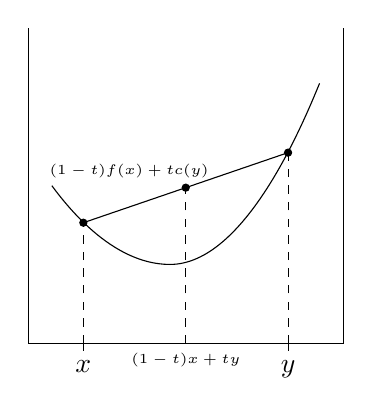
\begin{tikzpicture}
      \draw(-2, 4) -- (-2, 0) -- (2, 0) -- (2, 4);
      \draw (-1.3, 0.1) -- (-1.3, -0.1) node [below] {$x$};
      \draw (1.3, 0.1) -- (1.3, -0.1) node [below] {$y$};
      \draw (-1.7, 2) parabola bend (-.2, 1) (1.7, 3.3);
      \draw [dashed] (-1.3, 0) -- (-1.3, 1.53) node [circ] {};
      \draw [dashed] (1.3, 0) -- (1.3, 2.42) node [circ] {};
      \draw (-1.3, 1.53) -- (1.3, 2.42);
      \draw [dashed] (0, 0) node [below] {\tiny $(1 - t)x + ty$} -- (0, 1.975) node [above] {\tiny$(1 - t)f(x) + t c(y)\quad\quad\quad\quad\quad\quad$} node [circ] {};
    \end{tikzpicture}
  \end{center}
\end{defi}
Note that if $c$ is twice differentiable, then this is equivalent to $c'' > 0$.

\begin{prop}[Jensen's inequality]\index{Jensen's inequality}
  Let $X$ be an integrable random variable with values in $I$. If $c: I \to \R$ is convex, then we have
  \[
    \E[c(X)] \geq c(E[X]).
  \]
\end{prop}
It is crucial that this only applies to a probability space. We need the total mass of the measure space to be $1$ for it to work. Just being finite is not enough. Jensen's inequality will be an easy consequence of the following lemma:
\begin{lemma}
  If $c: I \to \R$ is a convex function and $m$ is in the interior of $I$, then there exists real numbers $a, b$ such that
  \[
    c(x) \geq ax + b
  \]
  for all $x \in I$, with equality at $x = m$.
  \begin{center}
    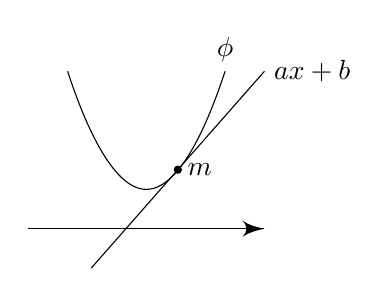
\begin{tikzpicture}
      \draw [->] (-1.5, 0) -- (1.5, 0);
      \draw (-1, 2) parabola bend (0, 0.5) (1, 2) node [above] {$\phi$};
      \node [circ] at (0.4, 0.75) {};
      \node [right] at (0.4, 0.75) {$m$};
      \draw (-0.7, -0.5) -- (1.5, 2) node [right] {$ax + b$};
    \end{tikzpicture}
  \end{center}
\end{lemma}
If the function is differentiable, then we can easily extract this from the derivative. However, if it is not, then we need to be more careful.

\begin{proof}
  If $c$ is smooth, then we know $c'' \geq 0$, and thus $c'$ is non-decreasing. We are going to show an analogous statement that does not mention the word ``derivative''. Consider $x < m < y$ with $x, y, m \in I$. We want to show that
   \[
    \frac{c(m) - c(x)}{m - x} \leq \frac{c(y) - c(m)}{y - m}.
  \]
  To see this, take
  \[
    t = \frac{y - m}{y - x}.
  \]
  Then by our choice of $x, m , y$, we know $t$ lies in $(0, 1)$, and
  \[
    m = tx + (1 - t) y.
  \]
  By convexity, we know
  \[
    c(m) = c(tx + (1 - t) y) \leq tc(x) + (1 - t) c(y).
  \]
  We can rewrite the LHS as
  \[
    c(m) = t c(m) + (1 - t) c(m).
  \]
  Rearranging, we find that
  \[
    t (c(m) - c(x)) \leq (1 - t)(c(y) - c(m)).
  \]
  Writing out the definition of $t$, we have
  \[
    \frac{y - m}{y - x} (c(m) - c(x)) \leq \frac{m - x}{y - x} (c(y) - c(m)).
  \]
  Cancelling the $y - x$ and dividing by the factors gives
  \[
    \frac{c(m) - c(x)}{m - x} \leq \frac{c(y) - c(m)}{y - m}.
  \]
  What does this say? If our $c$ is smooth, then if $c$ is convex, then $c'' \geq 0$. So $c'$ is non-decreasing. Here in our formula, both sides look like derivatives.

  Now since $x$ and $y$ are arbitrary, we know there is some $a \in \R$ such that
  \[
    \frac{c(m) - c(x)}{m - x} \leq a \leq \frac{c(y) - c(m)}{y - m}.
  \]
  for all $x < m < y$. This does the job. If we rearrange, then we obtain
  \[
    c(t) \geq a(t - m) + c(m)
  \]
  for all $t \in I$.
\end{proof}

\begin{proof}[Proof of Jensen's inequality]
  To apply the previous result, we need to pick a right $m$. We take
  \[
    m = \E [X].
  \]
  To apply this, we need to know that $m$ is in the interior of $I$. So we assume that $X$ is \emph{not} a.s. constant (that case is boring). By the lemma, we can find some $a, b \in \R$ such that
  \[
    c(X) \geq aX + b.
  \]
  We want to take the expectation of the LHS, but we have to make sure the $\E[c(X)]$ is a sensible thing to talk about. To make sure it makes sense, we show that $\E[c(X)^-] = \E[(-c(X)) \vee 0]$ is finite.

  We simply bound
  \[
    [c(X)]^- = [-c(X)] \vee 0 \leq |a| |X| + |b|.
  \]
  So we have
  \[
    \E[c(X)^-] \leq |a| \E |X| + |b| < \infty
  \]
  since $X$ is integrable. So $\E[c(X)]$ makes sense.

  We then just take
  \[
    \E[c(X)] \geq \E[aX + b] = a\E[X] + b = am + b = c(m) = c(\E[X]).
  \]
  So done.
\end{proof}

We are now going to use Jensen's inequality to prove H\"older's inequality. Before that, we take note of the following definition:
\begin{defi}[Conjugate]\index{conjugate}
  Let $p, q \in [1, \infty]$. We say that they are \emph{conjugate} if
  \[
    \frac{1}{p} + \frac{1}{q} = 1,
  \]
  where we take $1/\infty = 0$.
\end{defi}

\begin{prop}[H\"older's inequality]\index{H\"older's inequality}
  Let $p, q \in (1, \infty)$ be conjugate. Then for $f, g$ measurable, we have
  \[
    \mu(|fg|) = \|fg\|_1 \leq \|f\|_p \|g\|_q.
  \]
  When $p = q = 2$, then this is the Cauchy-Schwarz inequality.
\end{prop}

The proof is some magic, unenlightening manipulations.
\begin{proof}
  We assume that $\|f\|_p > 0$ and $\|f\|_p < \infty$. Otherwise, there is nothing to prove. By scaling, we may assume that $\|f\|_p = 1$. We make up a probability measure by
  \[
    \P[A] = \int |f|^p \mathbf{1}_A \;\d \mu.
  \]
  Since we know
  \[
    \|f\|_p = \left(\int |f|^p\;\d \mu\right)^{1/p} = 1,
  \]
  we know $\P[\ph]$ is a probability measure. Then we have
  \begin{align*}
    \mu(|fg|) &= \mu(|fg| \mathbf{1}_{\{|f| > 0\}})\\
    &= \mu\left(\frac{|g|}{|f|^{p - 1}} \mathbf{1}_{\{|f| > 0\}} |f|^p\right)\\
    &= \E\left[\frac{|g|}{|f|^{p - 1}}\mathbf{1}_{\{|f| > 0\}}\right]\\
    \intertext{Now use the fact that $(\E|X|)^q \leq \E[|X|^q]$ since $x \mapsto x^q$ is convex for $q > 1$. Then we obtain}
    &\leq \left(\E\left[\frac{|g|^q}{|f|^{(p - 1)q}}\mathbf{1}_{\{|f| > 0\}}\right]\right)^{1/q}.
  \end{align*}
  The key realization now is that $\frac{1}{q} + \frac{1}{p} = 1$ means that $q(p - 1) = p$. So this becomes
  \[
    \E\left[\frac{|g|^q}{|f|^p} \mathbf{1}_{\{|f| > 0\}}\right]^{1/q} = \mu(|g|^q)^{1/q} = \|g\|_q.
  \]
  Using the fact that $\|f\|_p = 1$, we obtain the desired result.
\end{proof}

Just like Jensen's inequality, this is very useful when bounding integrals, and it is also theoretically very important, because we are going to use it to prove the Minkowski inequality. This tells us that the $L^p$ norm is actually a norm.

Before we prove the Minkowski inequality, we prove the following tiny lemma that we will use repeatedly:
\begin{lemma}
  Let $a, b \geq 0$ and $p \geq 1$. Then
  \[
    (a + b)^p \leq 2^p(a^p + b^p).
  \]
\end{lemma}
This is a terrible bound, but is useful when we want to prove that things are finite.

\begin{proof}
  We wlog $a \leq b$. Then
  \[
    (a + b)^p \leq (2b)^p \leq 2^p b^p \leq 2^p(a^p + b^p).
  \]
\end{proof}
\begin{thm}[Minkowski inequality]\index{Minkowski inequality}
  Let $p \in [1, \infty]$ and $f, g$ measurable. Then
  \[
    \|f + g\|_p \leq \|f\|_p + \|g\|_p.
  \]
\end{thm}

Again the proof is magic.
\begin{proof}
  We do the boring cases first. If $p = 1$, then
  \[
    \|f + g\|_1 = \int |f + g| \leq \int (|f| + |g|) = \int |f| + \int |g| = \|f\|_1 + \|g\|_1.
  \]
  The proof of the case of $p = \infty$ is similar. Now assume $p \in (1, \infty)$. We assume that $\|f\|_p, \|g\|_p< \infty$, or else the inequality is trivial. Similarly, we assume $\|f + g\|_p > 0$.

  We now check that under these assumption, we must have $\|f + g\|_p < \infty$ as well. Indeed, we have
  \[
    |f + g|^p \leq (|f| + |g|)^p \leq 2^p(|f|^p + |g|^p).
  \]
  Then the claim follows by integrating both sides.

  So take $q$ conjugate to $p$. We then look at
  \[
    \||f + g|^{p - 1}\|_q = \mu(|f + g|^{(p - 1)q})^{1/q} = \mu(|f + g|^p)^{1 - 1/p}.
  \]
  We now use this in a clever way. We have
  \begin{align*}
    \mu(|f + g|^p) &= \mu(|f + g| |f + g|^{p - 1}) \\
    &\leq \mu(|f||f + g|^{p - 1}) + \mu(|g||f + g|^{p - 1})\\
    &\leq \|f\|_p \||f + g|^{p - 1}\|_q + \|g\|_p \||f + g|^{p - 1}\|_q\\
    &= (\|f\|_p + \|g\|_p) \||f + g|^{p - 1}\|_q\\
    &= (\|f\|_p + \|g\|_p) \mu(|f + g|^p)^{1 - 1/p}.
  \end{align*}
  So we know
  \[
    \mu(|f + g|^p) \leq (\|f\|_p + \|g\|_p) \mu(|f + g|^p)^{1 - 1/p}.
  \]
  Then dividing both sides by $(\mu(|f + g|^p)^{1 - 1/p}$ tells us
  \[
    \mu(|f + g|^p)^{1/p} = \|f + g\|_p \leq \|f\|_p + \|g\|_p.
  \]
\end{proof}

Given these inequalities, we can go and prove some properties of $L^p$ spaces.

\subsection{\tph{$L^p$}{Lp}{L<sup>p</sup>} spaces}
Recall the following definition:

\begin{defi}[Norm of vector space]\index{norm!vector space}\index{vector space!norm}
  Let $V$ be a vector space. A \emph{norm} on $V$ is a function $\|\ph\|: V \to \R_{\geq 0}$ such that
  \begin{enumerate}
    \item $\|u + v\| \leq \norm{u} + \norm{v}$ for all $U, v \in V$.
    \item $\|\alpha v\| = |\alpha|\|v\|$ for all $v \in V$ and $\alpha \in \R$
    \item $\|v\| = 0$ implies $v = 0$.
  \end{enumerate}
\end{defi}

\begin{defi}[$L^p$ spaces]\index{$L^p$ space}\index{$\|f\|_p$}
  Let $(E, \mathcal{E}, \mu)$ be a measurable space. For $1 \leq p < \infty$, we define $L^p = L^p(E, \mathcal{E}, \mu)$ to be the set of all measurable functions $f$ such that
  \[
    \|f\|_p = \left(\int |f|^p \d \mu\right)^{1/p} < \infty.
  \]
  For $p = \infty$, we let $L^\infty = L^\infty(E, \mathcal{E}, \mu)$ to be the space of functions with
  \[
    \|f\|_{\infty} = \inf \{\lambda \geq 0: |f| \leq \lambda \text{ a.e.}\} < \infty.
  \]
\end{defi}

By Minkowski's inequality, we know $L^p$ is a vector space, and also (i) holds. By definition, (ii) holds obviously. However, (iii) does \emph{not} hold for $\|\ph\|_p$, because $\|f\|_p = 0$ does not imply that $f = 0$. It merely implies that $f = 0$ a.e.

To fix this, we define an equivalence relation as follows: for $f, g \in L^p$, we say that $f \sim g$ iff $f - g = 0$ a.e. For any $f \in L^p$, we let $[f]$ denote its equivalence class under this relation. In other words,
\[
  [f] = \{g \in L^p: f - g = 0\text{ a.e.}\}.
\]
\begin{defi}[$\mathcal{L}^p$ space]\index{$\mathcal{L}^p$ space}
  We define
  \[
    \mathcal{L}^p = \{[f]: f \in L^p\},
  \]
  where
  \[
    [f] = \{g \in L^p: f - g = 0\text{ a.e.}\}.
  \]
  This is a normed vector space under the $\|\ph\|_p$ norm.
\end{defi}

One important property of $L^p$ is that it is complete, i.e.\ every Cauchy sequence converges.
\begin{defi}[Complete vector space/Banach spaces]\index{complete vector space}\index{Banach space}
  A normed vector space $(V, \|\ph\|)$ is \emph{complete} if every Cauchy sequence converges. In other words, if $(v_n)$ is a sequence in $V$ such that $\|v_n - v_m\| \to 0$ as $n, m \to \infty$, then there is some $v \in V$ such that $\|v_n - v\| \to 0$ as $n \to \infty$. A complete vector space is known as a \emph{Banach space}.
\end{defi}

\begin{thm}
  Let $1 \leq p \leq \infty$. Then $\mathcal{L}^p$ is a Banach space. In other words, if $(f_n)$ is a sequence in $L^p$, with the property that $\|f_n - f_m\|_p \to 0$ as $n, m \to \infty$, then there is some $f \in L^p$ such that $\|f_n - f\|_p \to 0$ as $n \to \infty$.
\end{thm}

\begin{proof}
  We will only give the proof for $p < \infty$. The $p = \infty$ case is left as an exercise for the reader.

  Suppose that $(f_n)$ is a sequence in $L^p$ with $\|f_n - f_m\|_p \to 0$ as $n, m \to \infty$. Take a subsequence $(f_{n_k})$ of $(f_n)$ with
  \[
    \|f_{n_{k + 1}} - f_{n_k}\|_p \leq 2^{-k}
  \]
  for all $k \in \N$. We then find that
  \[
    \norm{\sum_{k = 1}^M |f_{n_{k + 1}} - f_{n_k}|}_p \leq \sum_{k = 1}^M \|f_{n_{k + 1}} - f_{n_k}\|_p \leq 1.
  \]
  We know that
  \[
    \sum_{k = 1}^M |f_{n_{k + 1}} - f_{n_k}| \nearrow \sum_{k = 1}^\infty |f_{n_{k + 1}} - f_{n_k}|\text{ as }M \to \infty.
  \]
  So applying the monotone convergence theorem, we know that
  \[
    \norm{\sum_{k = 1}^\infty |f_{n_{k + 1}} - f_{n_k}|}_p \leq \sum_{k = 1}^\infty \|f_{n_{k + 1}} - f_{n_k}\|_p \leq 1.
  \]
  In particular,
  \[
    \sum_{k = 1}^\infty |f_{n_{k + 1}} - f_{n_k}| < \infty \text{ a.e.}
  \]
  So $f_{n_k}(x)$ converges a.e., since the real line is complete. So we set
  \[
    f(x) =
    \begin{cases}
      \lim_{k \to \infty} f_{n_k}(x) & \text{if the limit exists}\\
      0 & \text{otherwise}
    \end{cases}
  \]
  By an exercise on the first example sheet, this function is indeed measurable. Then we have
  \begin{align*}
    \|f_n - f\|_p^p &= \mu(|f_n - f|^p) \\
    &= \mu\left(\liminf_{k \to \infty} |f_n - f_{n_k}|^p\right)\\
    &\leq \liminf_{k \to \infty} \mu(|f_n - f_{n_k}|^p),
  \end{align*}
  which tends to $0$ as $n \to \infty$ since the sequence is Cauchy. So $f$ is indeed the limit.

  Finally, we have to check that $f \in L^p$. We have
  \begin{align*}
    \mu(|f|^p) &= \mu(|f - f_n + f_n|^p)\\
    &\leq \mu((|f - f_n| + |f_n|)^p)\\
    &\leq \mu(2^p (|f - f_n|^p + |f_n|^p))\\
    &= 2^p (\mu(|f - f_n|^p) + \mu(|f_n|^p)^2)
  \end{align*}
  We know the first term tends to $0$, and in particular is finite for $n$ large enough, and the second term is also finite. So done.
\end{proof}

\subsection{Orthogonal projection in \tph{$\mathcal{L}^2$}{L2}{L<sup>2</sup>}}
In the particular case $p = 2$, we have an extra structure on $\mathcal{L}^2$, namely an inner product structure, given by
\[
  \bra f, g\ket = \int fg\;\d \mu.
\]
This inner product induces the $L^2$ norm by
\[
  \|f\|_2^2 = \bra f, f\ket.
\]
Recall the following definition:
\begin{defi}[Hilbert space]\index{Hilbert space}
  A \emph{Hilbert space} is a vector space with a complete inner product.
\end{defi}
So $\mathcal{L}^2$ is not only a Banach space, but a Hilbert space as well.

Somehow Hilbert spaces are much nicer than Banach spaces, because you have an inner product structure as well. One particular thing we can do is orthogonal complements.

\begin{defi}[Orthogonal functions]\index{orthogonal functions}
  Two functions $f, g \in \mathcal{L}^2$ are \emph{orthogonal} if
  \[
    \bra f, g\ket = 0,
  \]
\end{defi}

\begin{defi}[Orthogonal complement]\index{orthogonal complement}\index{$V^\perp$}
  Let $V \subseteq L^2$. We then set
  \[
    V^\perp = \{f \in L^2: \bra f, v \ket = 0\text{ for all }v \in V\}.
  \]
\end{defi}

Note that we can always make these definitions for any inner product space. However, the completeness of the space guarantees nice properties of the orthogonal complement.

Before we proceed further, we need to make a definition of what it means for a subspace of $L^2$ to be closed. This isn't the usual definition, since $L^2$ isn't really a normed vector space, so we need to accommodate for that fact.

\begin{defi}[Closed subspace]\index{closed subspace}
  Let $V \subseteq L^2$. Then $V$ is closed if whenever $(f_n)$ is a sequence in $V$ with $f_n \to f$, then there exists $v \in V$ with $v \sim f$.
\end{defi}

Thee main thing that makes $L^2$ nice is that we can use closed subspaces to decompose functions orthogonally.

\begin{thm}
  Let $V$ be a closed subspace of $L^2$. Then each $f \in L^2$ has an \term{orthogonal decomposition}
  \[
    f = u + v,
  \]
  where $v \in V$ and $u \in V^\perp$. Moreover,
  \[
    \|f - v\|_2 \leq \|f - g\|_2
  \]
  for all $g \in V$ with equality iff $g \sim v$.
\end{thm}

To prove this result, we need two simple identities, which can be easily proven by writing out the expression.
\begin{lemma}[Pythagoras identity]\index{Pythagoras identity}
  \[
    \|f + g\|^2 = \|f\|^2 + \|g\|^2 + 2 \bra f, g\ket.
  \]
\end{lemma}

\begin{lemma}[Parallelogram law]\index{parallelogram law}
  \[
    \|f + g\|^2 + \|f - g\|^2 = 2(\|f\|^2 + \|g\|^2).
  \]
\end{lemma}

To prove the existence of orthogonal decomposition, we need to use a slight trick involving the parallelogram law.

\begin{proof}[Proof of orthogonal decomposition]
  Given $f \in L^2$, we take a sequence $(g_n)$ in $V$ such that
  \[
    \|f - g_n\|_2 \to d(f, V) = \inf_g \|f - g\|_2.
  \]
  We now want to show that the infimum is attained. To do so, we show that $g_n$ is a Cauchy sequence, and by the completeness of $L^2$, it will have a limit.

  If we apply the parallelogram law with $u = f - g_n$ and $v = f - g_m$, then we know
  \[
    \|u + v\|^2_2 + \|u - v\|_2^2 = 2(\|u\|^2_2 + \|v\|_2^2).
  \]
  Using our particular choice of $u$ and $v$, we obtain
  \[
    \norm{2 \left(f - \frac{g_n + g_m}{2}\right)}_2^2 + \|g_n - g_m\|_2^2 = 2(\|f - g_n\|_2^2 + \|f - g_m\|^2_2).
  \]
  So we have
  \[
    \|g_n - g_m\|_2^2 = 2(\|f - g_n\|_2^2 + \|f - g_m\|^2_2) - 4\norm{f - \frac{g_n + g_m}{2}}_2^2.
  \]
  The first two terms on the right hand side tend to $d(f, V)^2$, and the last term is bounded below in magnitude by $4d(f, V)$. So as $n, m \to \infty$, we must have $\|g_n - g_m\|_2 \to 0$. By completeness of $\mathcal{L}^2$, there exists a $g \in L^2$ such that $g_n \to g$.

  Now since $V$ is assumed to be closed, we can find a $v \in V$ such that $g = v$ a.e. Then we know
  \[
    \|f - v\|_2 = \lim_{n \to \infty}\|f - g_n\|_2 = d(f, V).
  \]
  So $v$ attains the infimum. To show that this gives us an orthogonal decomposition, we want to show that
  \[
    u = f - v \in V^\perp.
  \]
  Suppose $h \in V$. We need to show that $\bra u, h\ket = 0$. We need to do another funny trick. Suppose $t \in \R$. Then we have
  \begin{align*}
    d(f, V)^2 &\leq \|f - (v + th)\|_2^2 \\
    &= \|f - v\|^2 + t^2 \|h\|_2^2 - 2t \bra f - v, h\ket.
  \end{align*}
  We think of this as a quadratic in $t$, which is minimized when
  \[
    t = \frac{\bra f - v, h\ket}{\|h\|^2_2}.
  \]
  But we know this quadratic is minimized when $t = 0$. So $\bra f - v, h\ket = 0$.
\end{proof}

We are now going to look at the relationship between conditional expectation and orthogonal projection.
\begin{defi}[Conditional expectation]\index{conditional expectation}
  Suppose we have a probability space $(\Omega, \mathcal{F}, \P)$, and $(G_n)$ is a collection of pairwise disjoint events with $\bigcup_n G_n = \Omega$. We let
  \[
    \mathcal{G} = \sigma(G_n: n \in \N).
  \]
  The \emph{conditional expectation} of $X$ given $\mathcal{G}$ is the random variable
  \[
    Y = \sum_{n = 1}^\infty \E[X \mid G_n] \mathbf{1}_{G_n},
  \]
  where
  \[
    \E[X \mid G_n] = \frac{\E [X \mathbf{1}_{G_n}]}{ \P[G_n]}\text{ for }\P[G_n] > 0.
  \]
\end{defi}
In other words, given any $x \in \Omega$, say $x \in G_n$, then $Y(x) = \E[X \mid G_n]$.

If $X \in L^2(\P)$, then $Y \in L^2(\P)$, and it is clear that $Y$ is $\mathcal{G}$-measurable. We claim that this is in fact the projection of $X$ onto the subspace $L^2(\mathcal{G}, \P)$ of $\mathcal{G}$-measurable $L^2$ random variables in the ambient space $L^2(\P)$.

\begin{prop}
  The conditional expectation of $X$ given $\mathcal{G}$ is the projection of $X$ onto the subspace $L^2(\mathcal{G}, \P)$ of $\mathcal{G}$-measurable $L^2$ random variables in the ambient space $L^2(\P)$.
\end{prop}
In some sense, this tells us $Y$ is our best prediction of $X$ given only the information encoded in $\mathcal{G}$.

\begin{proof}
  Let $Y$ be the conditional expectation. It suffices to show that $\E[(X - W)^2]$ is minimized for $W = Y$ among $\mathcal{G}$-measurable random variables. Suppose that $W$ is a $\mathcal{G}$-measurable random variable. Since
  \[
    \mathcal{G} = \sigma(G_n: n \in \N),
  \]
  it follows that
  \[
    W = \sum_{n = 1}^\infty a_n \mathbf{1}_{G_n}.
  \]
  where $a_n \in \R$. Then
  \begin{align*}
    \E[(X - W)^2] &= \E\left[\left(\sum_{n = 1}^\infty (X - a_n) \mathbf{1}_{G_n}\right)^2\right]\\
    &= \E\left[\sum_n (X^2 + a_n^2 - 2a_n X)\mathbf{1}_{G_n}\right]\\
    &= \E\left[\sum_n (X^2 + a_n^2 - 2a_n \E[X\mid G_n])\mathbf{1}_{G_n}\right]
  \end{align*}
  We now optimize the quadratic
  \[
    X^2 + a_n^2 - 2 a_n \E[X \mid G_n]
  \]
  over $a_n$. We see that this is minimized for
  \[
    a_n = \E[X \mid G_n].
  \]
  Note that this does not depend on what $X$ is in the quadratic, since it is in the constant term.

  Therefore we know that $\E[X\mid G_n]$ is minimized for $W = Y$.
\end{proof}

We can also rephrase variance and covariance in terms of the $L^2$ spaces.

Suppose $X, Y \in L^2(\P)$ with
\[
  m_X = \E[X],\quad m_Y = \E[Y].
\]
Then \term{variance} and \term{covariance} just correspond to $L^2$ inner product and norm. In fact, we have
\begin{align*}
  \var(X) &= \E[(X - m_X)^2] = \|X - m_X\|_2^2,\\
  \cov(X, Y) &= \E[(X - m_X)(Y - m_Y)] = \bra X - m_X, Y - m_Y\ket.
\end{align*}
More generally, the \term{covariance matrix} of a random vector $X = (X_1, \cdots, X_n)$ is given by
\[
  \var(X) =(\cov(X_i, X_j))_{ij}.
\]
On the example sheet, we will see that the covariance matrix is a positive definite matrix.

\subsection{Convergence in \tph{$L^1(\P)$}{L1(P)}{L<sup>1</sup>(&\#x2119;)} and uniform integrability}
What we are looking at here is the following question --- suppose $(X_n), X$ are random variables and $X_n \to X$ in probability. Under what extra assumptions is it true that $X_n$ also converges to $X$ in $L_1$, i.e.\ $\E[X_n - X] \to 0$ as $X \to \infty$?

This is not always true.

\begin{eg}
  If we take $(\Omega, \mathcal{F}, \P) = ((0, 1), \mathcal{B}((0, 1)), \text{Lebesgue})$, and
  \[
    X_n = n\mathbf{1}_{(0, 1/n)}.
  \]
  Then $X_n \to 0$ in probability, and in fact $X_n \to 0$ almost surely. However,
  \[
    \E[|X_n - 0|] = \E[X_n] = n \cdot \frac{1}{n} = 1,
  \]
  which does not converge to $1$.
\end{eg}

It turns out there is a precise condition that makes this true, known as uniform integrability.

\begin{defi}[$L^p$-bounded]\index{$L^p$-bounded}
  Let $\mathcal{X}$ be a family of random variables. Then we say $\mathcal{X}$ is $L^p$ bounded if
  \[
    \sup\{\|X\|_p: X \in \mathcal{X}\} < \infty.
  \]
\end{defi}

\begin{defi}[Uniformly integrable]\index{uniformly integrable}\index{UI}
  Let $\mathcal{X}$ be a family of random variables. Define
  \[
    I_\mathcal{X}(\delta) = \sup\{\E[|X|\mathbf{1}_A]: X \in \mathcal{X}, A \in \mathcal{F} \text{ with }\mathcal{P}[A] < \delta\}.
  \]
  Then we say $\mathcal{X}$ is \emph{uniformly integrable} if $\mathcal{X}$ is $L^1$-bounded, and $I_\mathcal{X}(\delta) \to 0$ as $\delta \to 0$.
\end{defi}
In some sense, this is ``uniform continuity for integration''.

\begin{prop}
  Let $\mathcal{X} = \{X\}$, where $X \in L^1(\P)$. Then $\mathcal{X}$ is uniformly integrable.
\end{prop}

\begin{proof}
   To see this, we need to show that for any $\varepsilon > 0$, there exists some $\delta > 0$ such that $\P[A] < \delta$ implies $\E[|X|\mathbf{1}_A] < \varepsilon$.

  Suppose not. Then there exists $\varepsilon > 0$ and a sequence $(A_n)$ in $\mathcal{F}$ where $\E[|X|\mathbf{1}_{A_n}] \geq \varepsilon$ for all $n$, and $\P[A_n] \leq 2^{-n}$. Then we have
  \[
    \varepsilon \leq \E[X \mathbf{1}_{\bigcup_{m \geq n} A_n}] \to \E[|X| \mathbf{1}_{A_m\text{ i.o.}}]
  \]
  by dominated convergence with dominating function $|X|$.

  On the other hand, since $\sum \P[A_n] < \infty$, by Borel--Cantelli, we know
  \[
    \P[A_n\text{ i.o.}] = 0.
  \]
  This is a contradiction. So done.
\end{proof}

It is then a simple corollary that
\begin{cor}
  Any finite collection of $L^1$ functions is uniformly integrable.
\end{cor}

It turns out that it isn't too hard to find uniformly integrable functions.

\begin{prop}
  Let $\mathcal{X}$ be an $L^p$-bounded family for some $p > 1$. Then $\mathcal{X}$ is uniformly integrable.
\end{prop}

\begin{proof}
  We let
  \[
    C = \sup\{\|X\|_p : X \in \mathcal{X}\} < \infty.
  \]
  Suppose that $X \in \mathcal{X}$ and $A \in \mathcal{F}$. We then have
  \[
    \E[|X|\mathbf{1}_A] = \leq \E[|X|^p]^{1/p} \P[A]^{1/q} \leq C \P[A]^{1/q}.
  \]
  by H\"older's inequality, where $p, q$ are conjugates. This is now a uniform bound depending only on $\P[A]$. So done.
\end{proof}

This is the best we can get. $L^1$ boundedness is not enough. Indeed, our earlier example
\[
  X_n = n \mathbf{1}_{(0, 1/n)},
\]
is $L^1$ bounded but not uniformly integrable. So $L^1$ boundedness is not enough.

We are now going to work towards showing that the extra assumption of uniform integrability gives us $L^1$-convergence and in fact this is necessary and sufficient.

Before we do that, we prove a lemma that rephrases what it means for something to be uniformly integrable.

\begin{lemma}
  Let $\mathcal{X}$ be a family of random variables. Then $\mathcal{X}$ is uniformly integrable if and only if
  \[
    \sup\{\E[|X|\mathbf{1}_{|X| > k}]: X \in \mathcal{X}\} \to 0
  \]
  as $k \to \infty$.
\end{lemma}

\begin{proof}
  Suppose that $\chi$ is uniformly integrable. We fix $\varepsilon > 0$, and take $\delta > 0$ such that
  \[
    I_\mathcal{X}(\delta) < \varepsilon.
  \]
  Take $k < \infty$ so that
  \[
    I_\mathcal{X}(1) = \sup\{\E[|X|]: X \in \mathcal{X}\} \leq k \delta.
  \]
  For $X \in \mathcal{X}$ and $A = \{|X| \geq k\}$, we have that
  \[
    \P[A] < \delta
  \]
  by the Chebyshev inequality. So we know
  \[
    \E[|X|\mathbf{1}_A] \leq \varepsilon.
  \]
  So we know
  \[
    \sup\{E[|X| \mathbf{1}_{|X| > k}] X \in \mathcal{X}\} \to 0
  \]
  as $k \to \infty$.

  Conversely, suppose that the condition in the lemma holds. We first show that $\mathcal{X}$ is $L^1$-bounded. We have
  \[
    \E[|X|] = \E[|X|(\mathbf{1}_{\{|X| \leq k\}} + \mathbf{1}_{\{|X| > k\}}] \leq k + \E[|X| \mathbf{1}_{\{|X| > k\}}] < \infty
  \]
  by picking a large enough $k$.

  Next, we fix $\varepsilon > 0$. We take $k$ such that
  \[
    \E[|X|\mathbf{1}_{\{|X| > k\}}] < \frac{\varepsilon}{2}
  \]
  for all $X \in \mathcal{X}$. We choose $\delta > 0$ such that
  \[
    k \delta < \frac{\varepsilon}{2}.
  \]
  Then for $X \in \mathcal{X}$ and $A \in \mathcal{F}$ with $\P[A] \leq \delta$, we have
  \begin{align*}
    \E[|X| \mathbf{1}_A] &= \E[|X|\mathbf{1}_A (\mathbf{1}_{|X| > k} + \mathbf{1}_{|X| \leq k})]\\
    &\leq \E[|X| \mathbf{1}_{|X| > k}] + k \P[A]\\
    &\leq \frac{\varepsilon}{2} + \frac{\varepsilon}{2}\\
    &= \varepsilon.
  \end{align*}
   So done.
\end{proof}

To prove our ultimate theorem, we first need the following result:
\begin{thm}[Bounded convegence theorem]\index{bounded convergence theorem}
  Suppose $X, (X_n)$ are random variables. Assume that there exists a (non-random) constant $C > 0$ such that $|X_n| \leq C$. If $X_n \to X$ in probability, then $X_n \to X$ in $L^1$.
\end{thm}
This is somewhat a ``baby version'' of dominated convergence, but we have a much stronger condition of $|X_n|$ bounded by a constant, rather than an integrable function.

\begin{proof}
  Let $\varepsilon > 0$. We then have
  \begin{align*}
    \P[|X| > C+ \varepsilon] &\leq \P[|X - X_n| + |X_n| > C + \varepsilon]\\
    &\leq \P[|X - X_n|> \varepsilon] + \P[|X_n| > C]
  \end{align*}
  We know the second term vanishes, while the first term $\to 0$ as $n \to \infty$. So we know
  \[
    \P[|X| > C + \varepsilon] = 0
  \]
  for all $\varepsilon$. Since $\varepsilon$ was arbitrary, we know $|X| \leq C$ a.s.

  Now fix an $\varepsilon > 0$, and take $N$ such that
  \[
    \P\left[|X_n - X| > \frac{\varepsilon}{2}\right] \leq \frac{\varepsilon}{4C}
  \]
  for $n \geq N$. Then for $n \geq N$, we have
  \begin{align*}
    \E[|X_n - X|] &= \E\left[|X_n - X|(\mathbf{1}_{\{|X_n - X| \leq \frac{\varepsilon}{2}\}} + \mathbf{1}_{\{|X_n - X| > \frac{\varepsilon}{2}\})}\right]\\
    &\leq \frac{\varepsilon}{2} + 2C \P\left[|X_n - X| > \frac{\varepsilon}{2}\right]\\
    &\leq \frac{\varepsilon}{2} + 2C \frac{\varepsilon}{4C}\\
    &= \varepsilon.
  \end{align*}
  So done.
\end{proof}

We now come to the main theorem on uniform integrability.
\begin{thm}
  Let $X, (X_n)$ be random variables. Then the following are equivalent:
  \begin{enumerate}
    \item $X_n, X \in L^1$ for all $n$ and $X_n \to X$ in $L^1$.
    \item $\{X_n\}$ is uniformly integrable and $X_n \to X$ in probability.
  \end{enumerate}
\end{thm}

\begin{proof}
  We first assume that $X_n, X$ are $L^1$ and $X_n \to X$ in $L^1$. We want to show that $\{X_n\}$ is uniformly integrable and $X_n \to X$ in probability.

  We first show that $X_n \to X$ in probability. This is just going to come from the Chebyshev inequality. For $\varepsilon > 0$. Then we have
  \[
    \P[|X - X_n| > \varepsilon] \leq \frac{\E[|X - X_n|]}{\varepsilon} \to 0
  \]
  as $n \to \infty$.

  Next we show that $\{X_n\}$ is uniformly integrable. Fix $\varepsilon > 0$. Take $N$ such that $n \geq N$ implies $\E[|X - X_n|] \leq \frac{\varepsilon}{2}$. Since \emph{finite} families of $L^1$ random variables are uniformly integrable, we can pick $\delta > 0$ such that $A \in \mathcal{F}$ and $\P[A] < \delta$ implies
  \[
    \E[X \mathbf{1}_A], \E[|X_n|\mathbf{1}_A] \leq \frac{\varepsilon}{2}
  \]
  for $n = 1, \cdots, N$.

  Now when $n > N$ and $A \in \mathcal{F}$ with $\P[A] \leq \delta$, then we have
  \begin{align*}
    \E[|X_n| \mathbf{1}_A] &\leq \E[|X - X_n| \mathbf{1}_A] + \E[|X|\mathbf{1}_A]\\
    &\leq \E[|X - X_n|] + \frac{\varepsilon}{2}\\
    &\leq \frac{\varepsilon}{2} + \frac{\varepsilon}{2}\\
    &= \varepsilon.
  \end{align*}
  So $\{X_n\}$ is uniformly integrable.

  \separator

  Assume that $\{X_n\}$ is uniformly integrable and $X_n \to X$ in probability.

  The first step is to show that $X \in L^1$. We want to use Fatou's lemma, but to do so, we want almost sure convergence, not just convergence in probability.

  Recall that we have previously shown that there is a subsequence $(X_{n_k})$ of $(X_n)$ such that $X_{n_k} \to X$ a.s. Then we have
  \[
    \E[|X|] = \E\left[\liminf_{k \to \infty} |X_{n_k}|\right] \leq \liminf_{k \to \infty} \E[|X_{n_k}|] < \infty
  \]
  since uniformly integrable families are $L^1$ bounded. So $\E[|X|] < \infty$, hence $X \in L^1$.

  Next we want to show that $X_n \to X$ in $L^1$. Take $\varepsilon > 0$. Then there exists $K \in (0, \infty)$ such that
  \[
    \E\left[|X| \mathbf{1}_{\{|X| > K\}}\right], \E\left[|X_n| \mathbf{1}_{\{|X_n| > K\}}\right] \leq \frac{\varepsilon}{3}.
  \]
  To set things up so that we can use the bounded convergence theorem, we have to invent new random variables
  \[
    X_n^K = (X_n \vee -K) \wedge K,\quad X^K = (X \vee -K)\wedge K.
  \]
  Since $X_n \to X$ in probability, it follows that $X_n^K \to X^K$ in probability.

  Now bounded convergence tells us that there is some $N$ such that $n \geq N$ implies
  \[
    \E[|X_n^K - X^K|] \leq \frac{\varepsilon}{3}.
  \]
  Combining, we have for $n \geq N$ that
  \[
    \E[|X_n - X|] \leq \E[|X_n^K - X^K|] + \E[|X|\mathbf{1}_{\{|X| \geq K\}}] + \E[|X_n|\mathbf{1}_{\{|X_n| \geq K\}}] \leq \varepsilon.
  \]
  So we know that $X_n \to X$ in $L^1$.
\end{proof}

The main application is that when $\{X_n\}$ is a type of stochastic process known as a \term{martingale}. This will be done in III Advanced Probability and III Stochastic Calculus.

\section{Fourier transform}
We now turn to the exciting topic of the Fourier transform. There are two main questions we want to ask --- when does the Fourier transform exist, and when we can recover a function from its Fourier transform.

Of course, not only do we want to know if the Fourier transform exists. We also want to know if it lies in some nice space, e.g.\ $L^2$.

It turns out that when we want to prove things about Fourier transforms, it is often helpful to ``smoothen'' the function by doing what is known as a \emph{Gaussian convolution}. So after defining the Fourier transform and proving some really basic properties, we are going to investigate convolutions and Gaussians for a bit (convolutions are also useful on their own, since they correspond to sums of independent random variables). After that, we can go and prove the actual important properties of the Fourier transform.

\subsection{The Fourier transform}
When talking about Fourier transforms, we will mostly want to talk about functions $\R^d \to \C$. So from now on, we will write $L^p$ for \emph{complex valued} Borel functions on $\R^d$ with
\[
  \|f\|_p = \left(\int_{\R^d} |f|^p\right)^{1/p} < \infty.
\]
The integrals of complex-valued function are defined on the real and imaginary parts separately, and satisfy the properties we would expect them to. The details are on the first example sheet.

\begin{defi}[Fourier transform]\index{Fourier transform}
  The \emph{Fourier transform} $\hat{f}: \R^d \to \C$ of $f \in L^1(\R^d)$ is given by
  \[
    \hat{f}(u) = \int_{\R^d}f(x) e^{i (u, x)}\;\d x,
  \]
  where $u \in \R^d$ and $(u, x)$ denotes the inner product, i.e.
  \[
    (u, x) = u_1 x_1 + \cdots + u_d x_d.
  \]
\end{defi}

Why do we care about Fourier transforms? Many computations are easier with $\hat{f}$ in place of $f$, especially computations that involve differentiation and convolutions (which are relevant to sums of independent random variables). In particular, we will use it to prove the central limit theorem.

More generally, we can define the Fourier transform of a measure:

\begin{defi}[Fourier transform of measure]\index{Fourier transform!of measure}
  The Fourier transform of a \emph{finite measure} $\mu$ on $\R^d$ is the function $\hat{\mu}: \R^d \to \C$ given by
  \[
    \hat{\mu}(u) = \int_{\R^d} e^{i(u, x)} \mu(\d x).
  \]
\end{defi}

In the context of probability, we give these things a different name:
\begin{defi}[Characteristic function]\index{characteristic function}\index{random variable!characteristic function}
  Let $X$ be a random variable. Then the \emph{characteristic function} of $X$ is the Fourier transform of its law, i.e.
  \[
    \phi_X(u) = \E[e^{i(u, X)}] = \hat{\mu}_X(u),
  \]
  where $\mu_X$ is the law of $X$.
\end{defi}

We now make the following (trivial) observations:
\begin{prop}
  \[
    \|\hat{f}\|_\infty \leq \|f\|_1, \quad \|\hat{\mu}\|_\infty \leq \mu(\R^d).
  \]
\end{prop}

Less trivially, we have the following result:
\begin{prop}
  The functions $\hat{f}, \hat{\mu}$ are continuous.
\end{prop}

\begin{proof}
  If $u_n \to u$, then
  \[
    f(x) e^{i(u_n, x)} \to f(x) e^{i(u, x)}.
  \]
  Also, we know that
  \[
    |f(x) e^{i(u_n, x)}| = |f(x)|.
  \]
  So we can apply dominated convergence theorem with $|f|$ as the bound.
\end{proof}

\subsection{Convolutions}
To actually do something useful about the Fourier transforms, we need to talk about convolutions.

\begin{defi}[Convolution of random variables]\index{convolution!random variable}\index{random variable!convolution}
  Let $\mu, \nu$ be probability measures. Their \emph{convolution} $\mu * \nu$ is the law of $X + Y$, where $X$ has law $\mu$ and $Y$ has law $\nu$, and $X, Y$ are independent. Explicitly, we have
  \begin{align*}
    \mu * \nu (A) &= \P[X + Y \in \mathcal{A}] \\
    &= \iint \mathbf{1}_{A}(x + y)\;\mu(\d x)\;\nu(\d y)
  \end{align*}
\end{defi}
Let's suppose that $\mu$ has a density function $f$ with respect to the Lebesgue measure. Then we have
\begin{align*}
  \mu * \nu(A) &= \iint \mathbf{1}_A(x + y) f(x) \;\d x\;\nu(\d y)\\
  &= \iint \mathbf{1}_A(x) f(x - y) \;\d x\;\nu(\d y)\\
  &= \int \mathbf{1}_A(x) \left(\int f(x - y)\;\nu (\d y)\right)\;\d x.
\end{align*}
So we know that $\mu * \nu$ has law
\[
  \int f(x - y)\;\nu (\d y).
\]
This thing has a name.
\begin{defi}[Convolution of function with measure]\index{convolution!function with measure}
  Let $f \in L^p$ and $\nu$ a probability measure. Then the \emph{convolution} of $f$ with $\mu$ is
  \[
    f * \nu(x) = \int f(x - y)\;\nu(\d y) \in L^p.
  \]
\end{defi}
Note that we do have to treat the two cases of convolutions separately, since a measure need not have a density, and a function need not specify a probability measure (it may not integrate to $1$).

We check that it is indeed in $L^p$. Since $\nu$ is a probability measure, Jensen's inequality says we have
\begin{align*}
  \|f * \nu\|_p^p &= \int \left(\int |f(x - y)| \nu(\d y)\right)^p \;\d x\\
  &\leq \iint |f(x - y)|^p \nu(\d y)\;\d x\\
  &= \iint |f(x - y)|^p \;\d x \;\nu (\d y)\\
  &= \|f\|_p^p \\
  &< \infty.
\end{align*}
In fact, from this computation, we see that
\begin{prop}
  For any $f \in L^p$ and $\nu$ a probability measure, we have
  \[
    \|f * \nu\|_p \leq \|f\|_p.
  \]
\end{prop}

The interesting thing happens when we try to take the Fourier transform of a convolution.
\begin{prop}
  \[
    \widehat{f * \nu}(u) = \hat{f}(u) \hat{\nu}(u).
  \]
\end{prop}

\begin{proof}
  We have
  \begin{align*}
    \widehat{f * \nu}(u) &= \int \left(\int f(x - y) \nu(\d y)\right) e^{i(u, x)}\;\d x\\
    &= \iint f(x - y) e^{i(u, x)} \;\d x\;\nu (\d y)\\
    &= \int \left(\int f(x - y) e^{i(u, x - y)} \;\d (x - y)\right) e^{i(u, y)}\;\mu(\d y)\\
    &= \int \left(\int f(x) e^{i(u, x)} \;\d (x)\right) e^{i(u, y)}\;\mu(\d y)\\
    &= \int \hat{f}(u) e^{i(u, x)}\;\mu(\d y)\\
    &= \hat{f}(u) \int e^{i(u, x)}\;\mu(\d y)\\
    &= \hat{f}(u) \hat{\nu}(u).
  \end{align*}
\end{proof}

In the context of random variables, we have a similar result:
\begin{prop}
  Let $\mu, \nu$ be probability measures, and $X, Y$ be independent variables with laws $\mu, \nu$ respectively. Then
  \[
    \widehat{\mu * \nu}(u) = \hat{\mu}(u) \hat{\nu}(u).
  \]
\end{prop}

\begin{proof}
  We have
  \[
    \widehat{\mu * \nu}(u) = \E[e^{i(u, X + Y)}] = \E[e^{i(u, X)}] \E[e^{i(u, Y)}] = \hat{\mu}(u) \hat{\nu}(u).
  \]
\end{proof}

\subsection{Fourier inversion formula}
We now want to work towards proving the Fourier inversion formula:
\begin{thm}[Fourier inversion formula]
  Let $f,\hat{f} \in L^1$. Then
  \[
    f(x) = \frac{1}{(2\pi)^d} \int \hat{f}(u) e^{-i(u, x)} \;\d u\text{ a.e.}
  \]
\end{thm}

Our strategy is as follows:
\begin{enumerate}
  \item Show that the Fourier inversion formula holds for a Gaussian distribution by direct computations.
  \item Show that the formula holds for Gaussian convolutions, i.e.\ the convolution of an arbitrary function with a Gaussian.
  \item We show that any function can be approximated by a Gaussian convolution.
\end{enumerate}
Note that the last part makes a lot of sense. If $X$ is a random variable, then convolving with a Gaussian is just adding $X + \sqrt{t}Z$, and if we take $t \to 0$, we recover the original function. What we have to do is to show that this behaves sufficiently well with the Fourier transform and the Fourier inversion formula that we will actually get the result we want.

\subsubsection*{Gaussian densities}
Before we start, we had better start by defining the Gaussian distribution.
\begin{defi}[Gaussian density]\index{Gaussian density}
  The \emph{Gaussian density} with variance $t$ is
  \[
    g_t(x) = \left(\frac{1}{2\pi t}\right)^{d/2} e^{-|x|^2/2t}.
  \]
  This is equivalently the density of $\sqrt{t} Z$, where $Z = (Z_1, \cdots, Z_d)$ with $Z_i \sim N(0, 1)$ independent.
\end{defi}

We now want to compute the Fourier transformation directly and show that the Fourier inversion formula works for this.

We start off by working in the case $d = 1$ and $Z \sim N(0, 1)$. We want to compute the Fourier transform of the law of this guy, i.e.\ its characteristic function. We will use a nice trick.

\begin{prop}
  Let $Z \sim N(0, 1)$. Then
  \[
    \phi_Z(a) = e^{-u^2/2}.
  \]
\end{prop}
We see that this is in fact a Gaussian up to a factor of $2\pi$.

\begin{proof}
  We have
  \begin{align*}
    \phi_Z(u) &= \E[e^{iuZ}]\\
    &= \frac{1}{\sqrt{2\pi}} \int e^{iux} e^{-x^2/2}\;\d x.
  \end{align*}
  We now notice that the function is bounded, so we can differentiate under the integral sign, and obtain
  \begin{align*}
    \phi_Z'(u) &= \E[iZ e^{iuZ}]\\
    &= \frac{1}{\sqrt{2\pi}} \int ix e^{iux} e^{-x^2/2}\;\d x\\
    &= - u\phi_Z(u),
  \end{align*}
  where the last equality is obtained by integrating by parts. So we know that $\phi_Z(u)$ solves
  \[
    \phi_Z'(u) = -u \phi_Z(u).
  \]
  This is easy to solve, since we can just integrate this. We find that
  \[
    \log \phi_Z(u) = - \frac{1}{2}u^2 + C.
  \]
  So we have
  \[
    \phi_Z(u) = A e^{-u^2/2}.
  \]
  We know that $A = 1$, since $\phi_Z(0) = 1$. So we have
  \[
    \phi_Z(u) = e^{-u^2/2}.
  \]
\end{proof}

We now do this problem in general.
\begin{prop}
  Let $Z = (Z_1, \cdots, Z_d)$ with $Z_j \sim N(0, 1)$ independent. Then $\sqrt{t} Z$ has density
  \[
    g_t(x) = \frac{1}{(2\pi t)^{d/2}} e^{-|x|^2/(2t)}.
  \]
  with
  \[
    \hat{g}_t(u) = e^{-|u|^2 t/2}.
  \]
\end{prop}

\begin{proof}
  We have
  \begin{align*}
    \hat{g}_t(u) &= \E[e^{i(u, \sqrt{t}Z)}]\\
    &= \prod_{j = 1}^d \E[e^{i(u_j, \sqrt{t} Z_j)}]\\
    &= \prod_{j = 1}^d \phi_Z(\sqrt{t} u_j)\\
    &= \prod_{j = 1}^d e^{-t u_j^2/2}\\
    &= e^{-|u|^2 t/2}.
  \end{align*}
\end{proof}
Again, $g_t$ and $\hat{g}_t$ are almost the same, apart form the factor of $(2\pi t)^{-d/2}$ and the position of $t$ shifted. We can thus write this as
\[
  \hat{g}_t(u) = (2\pi)^{d/2} t^{-d/2} g_{1/t} (u).
\]
So this tells us that
\[
  \hat{\hat{g}}_t(u) = (2\pi)^d g_t(u).
\]
This is not exactly the same as saying the Fourier inversion formula works, because in the Fourier inversion formula, we integrated against $e^{-i(u, x)}$, not $e^{i(u, x)}$. However, we know that by the symmetry of the Gaussian distribution, we have
\[
  g_t(x) = g_t(-x) = (2\pi)^{-d} \hat{\hat{g}}_t (-x) = \left(\frac{1}{2\pi}\right)^d \int \hat{g}_t(u) e^{-i(u, x)}\;\d u.
\]
So we conclude that
\begin{lemma}
  The Fourier inversion formula holds for the Gaussian density function.
\end{lemma}

\subsubsection*{Gaussian convolutions}
\begin{defi}[Gaussian convolution]\index{Gaussian convolution}
  Let $f \in L^1$. Then a \emph{Gaussian convolution} of $f$ is a function of the form $f * g_t$.
\end{defi}

We are now going to do a little computation that shows that functions of this type also satisfy the Fourier inversion formula.

Before we start, we make some observations about the Gaussian convolution. By general theory of convolutions, we know that we have
\begin{prop}
  \[
    \|f * g_t\|_1 \leq \|f\|_1.
  \]
\end{prop}
We also have a pointwise bound
\begin{align*}
  |f*g_t(x)| &= \left|\int f(x - y) e^{-|y|^2/(2t)} \left(\frac{1}{2\pi t}\right)^{d/2} \;\d y\right| \\
  &\leq (2\pi t)^{-d/2} \int |f(x - y)| \;\d x\\
  &\leq (2\pi t)^{-d/2} \|f\|_1.
\end{align*}
This tells us that in fact
\begin{prop}
  \[
    \|f * g_t\|_\infty \leq (2\pi t)^{-d/2} \|f\|_1.
  \]
\end{prop}
So in fact the convolution is pointwise bounded. We see that the bound gets worse as $t \to 0$, and we will see that this is because as $t \to 0$, the convolution $f * g_t$ becomes a better and better approximation of $f$, and we did not assume that $f$ is bounded.

Similarly, we can compute that
\begin{prop}
  \[
    \|\widehat{f * g_t}\|_1 = \|\hat{f} \hat{g}_t\|_1 \leq (2\pi)^{d/2} t^{-d/2}\|\hat{f}\|_1,
  \]
  and
  \[
    \|\widehat{f * g_t}\|_\infty \leq \|\hat{f}\|_\infty.
  \]
\end{prop}
Now given these bounds, it makes sense to write down the Fourier inversion formula for a Gaussian convolution.
\begin{lemma}
  The Fourier inversion formula holds for Gaussian convolutions.
\end{lemma}

We are going to reduce this to the fact that the Gaussian distribution itself satisfies Fourier inversion.

\begin{proof}
  We have
  \begin{align*}
    f * g_t(x) &= \int f(x - y) g_t(y) \;\d y\\
    &= \int f(x - y) \left(\frac{1}{(2\pi)^d} \int \hat{g}_t(u) e^{-i(u, y)}\;\d u\right)\;\d y\\
    &= \left(\frac{1}{2\pi}\right)^d \iint f(x - y) \hat{g}_t(u) e^{-i(u, y)}\;\d u\;\d y\\
    &= \left(\frac{1}{2\pi}\right)^d \int \left(\int f(x - y) e^{-i(u, x - y)} \;\d y\right) \hat{g}_t(u) e^{-i(u, x)}\;\d u\\
    &= \left(\frac{1}{2\pi}\right)^d \int \hat{f}(u)\hat{g}_t(u) e^{-i(u, x)}\;\d u\\
    &= \left(\frac{1}{2\pi}\right)^d \int \widehat{f * g_t}(u) e^{-i(u, x)}\;\d u
  \end{align*}
  So done.
\end{proof}

\subsubsection*{The proof}
Finally, we are going to extend the Fourier inversion formula to the case where $f, \hat{f} \in L^2$.
\begin{thm}[Fourier inversion formula]
  Let $f \in L^1$ and
  \[
    f_t(x) = (2\pi)^{-d} \int \hat{f}(u) e^{-|u|^2 t/2} e^{-i(u, x)}\;\d u = (2\pi)^{-d} \int \widehat{f * g_t}(u) e^{-i(u, x)}\;\d u.
  \]
  Then $\|f_t - f\|_1 \to 0$, as $t \to 0$, and the Fourier inversion holds whenever $f, \hat{f} \in L^1$.
\end{thm}

To prove this, we first need to show that the Gaussian convolution is indeed a good approximation of $f$:
\begin{lemma}
  Suppose that $f \in L^p$ with $p \in [1, \infty)$. Then $\|f * g_t - f\|_p \to 0$ as $t \to 0$.
\end{lemma}
Note that this cannot hold for $p = \infty$. Indeed, if $p = \infty$, then the $\infty$-norm is the uniform norm. But we know that $f * g_t$ is always continuous, and the uniform limit of continuous functions is continuous. So the formula cannot hold if $f$ is not already continuous.

\begin{proof}
  We fix $\varepsilon > 0$. By a question on the example sheet, we can find $h$ which is continuous and with compact support such that $\|f - h\|_p \leq \frac{\varepsilon}{3}$. So we have
  \[
    \|f * g_t - h * g_t\|_p = \|(f - h) * g_t\|_p \leq \|f - h\|_p \leq \frac{\varepsilon}{3}.
  \]
  So it suffices for us to work with a continuous function $h$ with compact support. We let
  \[
    e(y) = \int |h(x - y) - h(x)|^p \;\d x.
  \]
  We first show that $e$ is a bounded function:
  \begin{align*}
    e(y) &\leq \int 2^p(|h(x - y)|^p + |h(x)|^p)\;\d x\\
    &= 2^{p + 1} \|h\|_p^p.
  \end{align*}
  Also, since $h$ is continuous and bounded, the dominated convergence theorem tells us that $e(y) \to 0$ as $y \to 0$.

  Moreover, using the fact that $\int g_t(y) \;\d y = 1$, we have
  \begin{align*}
    \|h*g_t - h\|_p^p &= \int \left|\int (h(x - y) - h(x))g_t(y) \;\d y\right|^p \;\d x\\
    \intertext{Since $g_t(y) \;\d y$ is a probability measure, by Jensen's inequality, we can bound this by}
    &\leq \iint |h(x - y) - h(x)|^p \;\d y \;\d x\\
    &= \int \left(\int |h(x - y) - h(x)|^p \;\d x\right) g_t(y) \;\d y\\
    &= \int e(y) g_t(y) \;\d y\\
    &= \int e(\sqrt{t} y) g_1(y)\;\d y,
  \end{align*}
  where we used the definition of $g$ and substitution. We know that this tends to $0$ as $t \to 0$ by the bounded convergence theorem, since we know that $e$ is bounded.

  Finally, we have
  \begin{align*}
    \|f * g_t - f\|_p &\leq \|f * g_t - h * g_t\|_p + \|h*g_t - h\|_p + \|h - f\|_p\\
    &\leq \frac{\varepsilon}{3} + \frac{\varepsilon}{3} + \|h*g_t - h\|_p\\
    &= \frac{2\varepsilon}{3} + \|h*g_t - h\|_p.
  \end{align*}
  Since we know that $\|h*g_t - h\|_p \to 0$ as $t \to 0$, we know that for all sufficiently small $t$, the function is bounded above by $\varepsilon$. So we are done.
\end{proof}

With this lemma, we can now prove the Fourier inversion theorem.
\begin{proof}[Proof of Fourier inversion theorem]
  The first part is just a special case of the previous lemma. Indeed, recall that
  \[
    \widehat{f * g_t} (u) = \hat{f}(u) e^{-|u|^2 t/2}.
  \]
  Since Gaussian convolutions satisfy Fourier inversion formula, we know that
  \[
    f_t = f * g_t.
  \]
  So the previous lemma says exactly that $\|f_t - f\|_1 \to 0$.

  Suppose now that $\hat{f} \in L^1$ as well. Then looking at the integrand of
  \[
    f_t(x) = (2\pi)^{-d} \int \hat{f}(u) e^{-|u|^2t/2} e^{-i(u, x)}\;\d u,
  \]
  we know that
  \[
    \left| \hat{f}(u) e^{-|u|^2t/2} e^{-i(u, x)}\right| \leq |\hat{f}|.
  \]
  Then by the dominated convergence theorem with dominating function $|\hat{f}|$, we know that this converges to
  \[
    f_t(x) \to (2\pi)^{-d} \int \hat{f}(u) e^{-i(u, x)}\;\d u\text{ as }t \to 0.
  \]
  By the first part, we know that $\|f_t - f\|_1 \to 0$ as $t \to 0$. So we can find a sequence $(t_n)$ with $t_n > 0$, $t_n \to 0$ so that $f_{t_n} \to f$ a.e. Combining these, we know that
  \[
    f(x) = \int \hat{f}(u) e^{-i(u, x)}\;\d u \text{ a.e.}
  \]
  So done.
\end{proof}

\subsection{Fourier transform in \tph{$\mathcal{L}^2$}{L2}{L<sup>2</sup>}}
It turns out wonderful things happen when we take the Fourier transform of an $L^2$ function.
\begin{thm}[Plancherel identity]\index{Plancherel identity}
  For any function $f \in L^1 \cap L^2$, the \emph{Plancherel identity} holds:
  \[
    \|\hat{f}\|_2 = (2\pi)^{d/2} \|f\|_2.
  \]
\end{thm}
As we are going to see in a moment, this is just going to follow from the Fourier inversion formula plus a clever trick.

\begin{proof}
  We first work with the special case where $f, \hat{f} \in L^1$, since the Fourier inversion formula holds for $f$. We then have
  \begin{align*}
    \|f\|_2^2 &= \int f(x) \overline{f(x)}\;\d x\\
    &= \frac{1}{(2\pi)^d} \int \left(\int \hat{f}(u) e^{-i(u, x)}\;\d u\right)\overline{f(x)}\;\d x\\
    &= \frac{1}{(2\pi)^d} \int \hat{f}(u) \left(\overline{f(x)} e^{-i(u, x)}\;\d x\right) \;\d u\\
    &= \frac{1}{(2\pi)^d} \int \hat{f}(u) \overline{\left(f(x) e^{i(u, x)}\;\d x\right)} \;\d u\\
    &= \frac{1}{(2\pi)^d} \int \hat{f}(u) \overline{\hat{f}(u)} \;\d u\\
    &= \frac{1}{(2\pi)^d} \|\hat{f}(u)\|_2^2.
  \end{align*}
  So the Plancherel identity holds for $f$.

  To prove it for the general case, we use this result and an approximation argument. Suppose that $f \in L^1 \cap L^2$, and let $f_t = f * g_t$. Then by our earlier lemma, we know that
  \[
    \|f_t\|_2 \to \|f\|_2\text{ as }t \to 0.
  \]
  Now note that
  \[
    \hat{f}_t(u) = \hat{f}(u)\hat{g}_t(u) = \hat{f}(u) e^{-|u|^2 t/2}.
  \]
  The important thing is that $e^{-|u|^2 t/2} \nearrow 1$ as $t \to 0$. Therefore, we know
  \[
    \|\hat{f}_t \|_2^2 = \int |\hat{f}(u)|^2 e^{-|u|^2 t}\; \d u \to \int |\hat{f}(u)|^2 \;\d u = \|\hat{f}\|_2^2
  \]
  as $t \to 0$, by monotone convergence.

  Since $f_t, \hat{f}_t \in L^1$, we know that the Plancherel identity holds, i.e.
  \[
    \|\hat{f}_t\|_2 = (2\pi)^{d/2} \|f_t\|_2.
  \]
  Taking the limit as $t \to 0$, the result follows.
\end{proof}

What is this good for? It turns out that the Fourier transform gives as a bijection from $\mathcal{L}^2$ to itself. While it is not true that the Fourier inversion formula holds for everything in $\mathcal{L}^2$, it holds for enough of them that we can just approximate everything else by the ones that are nice. Then the above tells us that in fact this bijection is a norm-preserving automorphism.

\begin{thm}
  There exists a unique Hilbert space automorphism $F: \mathcal{L}^2 \to \mathcal{L}^2$ such that
  \[
    F([f]) = [(2\pi)^{-d/2}\hat{f}]
  \]
  whenever $f \in L^1 \cap L^2$.

  Here $[f]$ denotes the equivalence class of $f$ in $\mathcal{L}^2$, and we say $F: \mathcal{L}^2 \to \mathcal{L}^2$ is a Hilbert space automorphism if it is a linear bijection that preserves the inner product.
\end{thm}
Note that in general, there is no guarantee that $F$ sends a function to its Fourier transform. We know that only if it is a well-behaved function (i.e.\ in $L^1 \cap L^2$). However, the formal property of it being a bijection from $\mathcal{L}^2$ to itself will be convenient for many things.

\begin{proof}
  We define $F_0: \mathcal{L}^1 \cap \mathcal{L}^2 \to \mathcal{L}^2$ by
  \[
    F_0([f]) = [(2\pi)^{-d/2} \hat{f}].
  \]
  By the Plancherel identity, we know $F_0$ preserves the $L^2$ norm, i.e.
  \[
    \|F_0([f])\|_2 = \|[f]\|_2.
  \]
  Also, we know that $\mathcal{L}^1 \cap \mathcal{L}^2$ is dense in $\mathcal{L}^2$, since even the continuous functions with compact support are dense. So we know $F_0$ extends uniquely to an isometry $F: \mathcal{L}^2 \to \mathcal{L}^2$.

  Since it preserves distance, it is in particular injective. So it remains to show that the map is surjective. By Fourier inversion, the subspace
  \[
    V = \{[f] \in \mathcal{L}^2: f, \hat{f} \in L^1\}
  \]
  is sent to itself by the map $F$. Also if $f \in V$, then $F^4[f] = [f]$ (note that applying it twice does not suffice, because we actually have $F^2[f](x) = [f](-x)$). So $V$ is contained in the image $F$, and also $V$ is dense in $\mathcal{L}^2$, again because it contains all Gaussian convolutions (we have $\hat{f_t} = \hat{f} \hat{g_t}$, and $\hat{f}$ is bounded and $\hat{g_t}$ is decaying exponentially). So we know that $F$ is surjective.
\end{proof}

\subsection{Properties of characteristic functions}
We are now going to state a bunch of theorems about characteristic functions. Since the proofs are not examinable (but the statements are!), we are only going to provide a rough proof sketch.

\begin{thm}
  The characteristic function $\phi_X$ of a distribution $\mu_X$ of a random variable $X$ determines $\mu_X$. In other words, if $X$ and $\tilde{X}$ are random variables and $\phi_X = \phi_{\tilde{X}}$, then $\mu_X = \mu_{\tilde{X}}$
\end{thm}

\begin{proof}[Proof sketch]
  Use the Fourier inversion to show that $\phi_X$ determines $\mu_X(g) = \E[g(X)]$ for any bounded, continuous $g$.
\end{proof}

\begin{thm}
  If $\phi_X$ is integrable, then $\mu_X$ has a bounded, continuous density function
  \[
    f_X(x) = (2\pi)^{-d} \int \phi_X(u) e^{-i(u, x)}\;\d u.
  \]
\end{thm}

\begin{proof}[Proof sketch]
  Let $Z \sim N(0, 1)$ be independent of $X$. Then $X + \sqrt{t} Z$ has a bounded continuous density function which, by Fourier inversion, is
  \[
    f_t(x) = (2\pi)^{-d} \int \phi_X(u) e^{-|u|^2 t / 2} e^{-i(u, x)}\;\d u.
  \]
  Sending $t \to 0$ and using the dominated convergence theorem with dominating function $|\phi_X|$.
\end{proof}

The next theorem relates to the notion of weak convergence.
\begin{defi}[Weak convergence of measures]\index{weak convergence!of measures}
  Let $\mu, (\mu_n)$ be Borel probability measures. We say that $\mu_n \to \mu$ \emph{weakly} if and only if $\mu_n(g) \to \mu(g)$ for all bounded continuous $g$.
\end{defi}

Similarly, we can define weak convergence of random variables.

\begin{defi}[Weak convergence of random variables]\index{weak convergence!of random variables}
  Let $X, (X_n)$ be random variables. We say $X_n \to X$ weakly iff $\mu_{X_n} \to \mu_X$ weakly, iff $\E[g(X_n)] \to \E[g(X)]$ for all bounded continuous $g$.
\end{defi}

This is related to the notion of convergence in distribution, which we defined long time ago without talking about it much. It is an exercise on the example sheet that weak convergence of random variables in $\R$ is equivalent to convergence in distribution.

It turns out that weak convergence is very useful theoretically. One reason is that they are related to convergence of characteristic functions.
\begin{thm}
  Let $X, (X_n)$ be random variables with values in $\R^d$. If $\phi_{X_n}(u) \to \phi_X(u)$ for each $u \in \R^d$, then $\mu_{X_n} \to \mu_X$ weakly.
\end{thm}

The main application of this that will appear later is that this is the fact that allows us to prove the central limit theorem.

\begin{proof}[Proof sketch]
  By the example sheet, it suffices to show that $\E[g(X_n)] \to \E[g(X)]$ for all compactly supported $g \in C^\infty$. We then use Fourier inversion and convergence of characteristic functions to check that
  \[
    \E[g(X_n + \sqrt{t}Z)] \to \E[g(X + \sqrt{t}Z)]
  \]
  for all $t > 0$ for $Z\sim N(0, 1)$ independent of $X, (X_n)$. Then we check that $\E[g(X_n + \sqrt{t}Z)]$ is close to $\E[g(X_n)]$ for $t > 0$ small, and similarly for $X$.
\end{proof}

\subsection{Gaussian random variables}
Recall that in the proof of the Fourier inversion theorem, we used these things called Gaussians, but didn't really say much about them. These will be useful later on when we want to prove the central limit theorem, because the central limit theorem says that in the long run, things look like Gaussians. So here we lay out some of the basic definitions and properties of Gaussians.

\begin{defi}[Gaussian random variable]\index{Gaussian random variable}\index{random variable!Gaussian}
  Let $X$ be a random variable on $\R$. This is said to be \emph{Gaussian} if there exists $\mu \in \R$ and $\sigma \in (0, \infty)$ such that the density of $X$ is
  \[
    f_X(x) = \frac{1}{\sqrt{2\pi \sigma^2}} \exp\left(-\frac{(x - \mu)^2}{2 \sigma^2}\right).
  \]
  A constant random variable $X = \mu$ corresponds to $\sigma = 0$. We say this has \term{mean} $\mu$ and \term{variance} $\sigma^2$.\index{Gaussian random variable!mean}\index{Gaussian random variable!variance}

  When this happens, we write $X \sim N(\mu, \sigma^2)$.\index{$N(\mu, \sigma^2)$}
\end{defi}

For completeness, we record some properties of Gaussian random variables.

\begin{prop}
  Let $X \sim N(\mu, \sigma^2)$. Then
  \[
    \E[X] = \mu,\quad \var(X) = \sigma^2.
  \]
  Also, for any $a, b \in \R$, we have
  \[
    aX + b \sim N(a\mu + b, a^2 \sigma^2).
  \]
  Lastly, we have
  \[
    \phi_X(u) = e^{-i\mu u - u^2 \sigma^2/2}.
  \]
\end{prop}

\begin{proof}
  All but the last of them follow from direct calculation, and can be found in IA Probability.

  For the last part, if $X \sim N(\mu, \sigma^2)$, then we can write
  \[
    X = \sigma Z + \mu,
  \]
  where $Z \sim N(0, 1)$. Recall that we have previously found that the characteristic function of a $N(0, 1)$ function is
  \[
    \phi_Z(u) = e^{-|u|^2/2}.
  \]
  So we have
  \begin{align*}
    \phi_X(u) &= \E[e^{iu(\sigma Z + \mu)}]\\
    &= e^{iu\mu} \E[e^{iu\sigma \Z}]\\
    &= e^{iu\mu} \phi_Z(iu\sigma)\\
    &= e^{iu \mu - u^2 \sigma^2/2}.
  \end{align*}
\end{proof}
What we are next going to do is to talk about the corresponding facts for the Gaussian in higher dimensions. Before that, we need to come up with the definition of a higher-dimensional Gaussian distribution. This might be different from the one you've seen previously, because we want to allow some degeneracy in our random variable, e.g.\ some of the dimensions can be constant.

\begin{defi}[Gaussian random variable]\index{Gaussian random variable}\index{random variable!Gaussian}
  Let $X$ be a random variable. We say that $X$ is a \emph{Gaussian on $\R^n$} if $(u, X)$ is Gaussian on $\R$ for all $u \in \R^n$.
\end{defi}

We are now going to prove a version of our previous theorem to higher dimensional Gaussians.
\begin{thm}
  Let $X$ be Gaussian on $\R^n$, and le t$A$ be an $m \times n$ matrix and $b \in \R^m$. Then
  \begin{enumerate}
    \item $AX + b$ is Gaussian on $\R^m$.
    \item $X \in L^2$ and its law $\mu_X$ is determined by $\mu = \E[X]$ and $V = \var(X)$, the covariance matrix.
    \item We have
      \[
        \phi_X(u) = e^{i(u, \mu) - (u, Vu)/2}.
      \]
    \item If $V$ is invertible, then $X$ has a density of
      \[
        f_X (x) = (2\pi)^{-n/2} (\det V)^{-1/2} \exp\left(-\frac{1}{2} (x - \mu, V^{-1}(x - \mu))\right).
      \]
    \item If $X = (X_1, X_2)$ where $X_i \in \R^{n_i}$, then $\cov(X_1, X_2) = 0$ iff $X_1$ and $X_2$ are independent.
  \end{enumerate}
\end{thm}
\begin{proof}\leavevmode
  \begin{enumerate}
    \item If $u \in \R^m$, then we have
      \[
        (AX + b, u) = (AX, u) + (b, u) = (X, A^T u) + (b, u).
      \]
      Since $(X, A^T u)$ is Gaussian and $(b, u)$ is constant, it follows that $(AX + b, u)$ is Gaussian.
    \item We know in particular that each component of $X$ is a Gaussian random variable, which are in $L^2$. So $X \in L^2$. We will prove the second part of (ii) with (iii)
    \item If $\mu = \E[X]$ and $V = \var(X)$, then if $u \in \R^n$, then we have
      \[
        \E[(u, X)] = (u, \mu),\quad \var((u, X)) = (u, Vu).
      \]
      So we know
      \[
        (u, X) \sim N((u, \mu), (u, Vu)).
      \]
      So it follows that
      \[
        \phi_X(u) = \E[e^{i(u, X)}] = e^{i(u, \mu) - (u, Vu)/2}.
      \]
      So $\mu$ and $V$ determine the characteristic function of $X$, which in turn determines the law of $X$.
    \item We start off with a boring Gaussian vector $Y = (Y_1, \cdots, Y_n)$, where the $Y_i \sim N(0, 1)$ are independent. Then the density of $Y$ is
      \[
        f_Y(y) = (2\pi)^{-n/2} e^{-|y|^2/2}.
      \]
      We are now going to construct $X$ from $Y$. We define
      \[
        \tilde{X} = V^{1/2} Y + \mu.
      \]
      This makes sense because $V$ is always non-negative definite. Then $\tilde{X}$ is Gaussian with $\E[\tilde{X}] = \mu$ and $\var(\tilde{X}) = V$. Therefore $X$ has the same distribution as $\tilde{X}$. Since $V$ is assumed to be invertible, we can compute the density of $\tilde{X}$ using the change of variables formula.
    \item It is clear that if $X_1$ and $X_2$ are independent, then $\cov(X_1, X_2) = 0$.

      Conversely, let $X = (X_1, X_2)$, where $\cov(X_1, X_2) = 0$. Then we have
      \[
        V = \var(X) =
        \begin{pmatrix}
          V_{11} & 0\\
          0 & V_{22}
        \end{pmatrix}.
      \]
      Then for $u = (u_1, u_2)$, we have
      \[
        (u, Vu) = (u_1 V_{11} u_1) + (u_2, V_{22}u_2),
      \]
      where $V_{11} = \var(X_1)$ and $V_{22} \var(X_2)$. Then we have
      \begin{align*}
        \phi_X(u) &= e^{i\mu u - (u, Vu)/2}\\
        &= e^{i\mu_1 u_1 - (u_1, V_{11}u_1)/2} e^{i\mu_2 u_2 - (u_2, V_{22}u_2)/2}\\
        &= \phi_{X_1}(u_1)\phi_{X_2} (u_2).
      \end{align*}
      So it follows that $X_1$ and $X_2$ are independent.
  \end{enumerate}
\end{proof}

\section{Ergodic theory}
We are now going to study a new topic --- ergodic theory. This is the study the ``long run behaviour'' of system under the evolution of some $\Theta$. Due to time constraints, we will not do much with it. We are going to prove two ergodic theorems that tell us what happens in the long run, and this will be useful when we prove our strong law of large numbers at the end of the course.

The general settings is that we have a measure space $(E, \mathcal{E}, \mu)$ and a measurable map $\Theta: E \to E$ that is measure preserving, i.e.\ $\mu(A) = \mu(\Theta^{-1}(A))$ for all $A \in \mathcal{E}$.

\begin{eg}
  Take $(E, \mathcal{E}, \mu) = ([0, 1), \mathcal{B}([0, 1)), \mathrm{Lebesgue})$. For each $a \in [0, 1)$, we can define
  \[
    \Theta_a (x) = x + a \mod 1.
  \]
  By what we've done earlier in the course, we know this translation map preserves the Lebesgue measure on $[0, 1)$.
\end{eg}

Our goal is to try to understand the ``long run averages'' of the system when we apply $\Theta$ many times. One particular quantity we are going to look at is the following:

Let $f$ be measurable. We define\index{$S_n(f)$}
\[
  S_n(f) = f + f \circ \Theta + \cdots + f \circ \Theta^{n - 1}.
\]
We want to know what is the long run behaviour of $\frac{S_n(f)}{n}$ as $n \to \infty$.

The \emph{ergodic theorems} are going to give us the answer in a certain special case. Finally, we will apply this in a particular case to get the strong law of large numbers.

\begin{defi}[Invariant subset]\index{invariant subset}
  We say $A \in \mathcal{E}$ is invariant for $\Theta$ if $A = \Theta^{-1}(A)$.
\end{defi}

\begin{defi}[Invariant function]\index{invariant function}
  A measurable function $f$ is invariant if $f = f \circ \Theta$.
\end{defi}

\begin{defi}[$\mathcal{E}_\Theta$]\index{$\mathcal{E}_\Theta$}
  We write
  \[
    \mathcal{E}_\Theta = \{A \in \mathcal{E}: A\text{ is invariant}\}.
  \]
\end{defi}
It is easy to show that $\mathcal{E}_\Theta$ is a $\sigma$-algebra, and $f: E \to \R$ is invariant iff it is $\mathcal{E}_\Theta$ measurable.

\begin{defi}[Ergodic]\index{ergodic}
  We say $\Theta$ is \emph{ergodic} if $A \in \mathcal{E}_\Theta$ implies $\mu(A) = 0$ or $\mu(A^C) = 0$.
\end{defi}

\begin{eg}
  For the translation map on $[0, 1)$, we have $\Theta_a$ is ergodic iff $a$ is irrational. Proof is left on example sheet 4.
\end{eg}

\begin{prop}
  If $f$ is integrable and $\Theta$ is measure-preserving. Then $f \circ \Theta$ is integrable and
  \[
    \int f \circ \Theta \d \mu = \int_E f \d \mu.
  \]
\end{prop}

It turns out that if $\Theta$ is ergodic, then there aren't that many invariant functions.
\begin{prop}
  If $\Theta$ is ergodic and $f$ is invariant, then there exists a constant $c$ such that $f = c$ a.e.
\end{prop}
The proofs of these are left as an exercise on example sheet $4$.

We are now going to spend a little bit of time studying a particular example, because this will be needed to prove the strong law of large numbers.

\begin{eg}[Bernoulli shifts]\index{Bernoulli shift}
  Let $m$ be a probability distribution on $\R$. Then there exists an iid sequence $Y_1, Y_2, \cdots$ with law $m$. Recall we constructed this in a really funny way. Now we are going to build it in a more natural way.

  We let $E = \R^\N$ be the set of all real sequences $(x_n)$. We define the $\sigma$-algebra $\mathcal{E}$ to be the $\sigma$-algebra generated by the projections $X_n(x) = x_n$. In other words, this is the smallest $\sigma$-algebra such that all these functions are measurable. Alternatively, this is the $\sigma$-algebra generated by the $\pi$-system
  \[
    \mathcal{A} = \left\{\prod_{n \in \N} A_n, A_n \in \mathcal{B}\text{ for all $n$ and $A_n = \R$ eventually}\right\}.
  \]
  Finally, to define the measure $\mu$, we let
  \[
    Y = (Y_1, Y_2, \cdots) : \Omega \to E
  \]
  where $Y_i$ are iid random variables defined earlier, and $\Omega$ is the sample space of the $Y_i$.

  Then $Y$ is a measurable map because each of the $Y_i$'s is a random variable. We let $\mu = \P \circ Y^{-1}$.

  By the independence of $Y_i$'s, we have that
  \[
    \mu(A) = \prod_{n \in \N} m(A_n)
  \]
  for any
  \[
    A = A_1 \times A_2 \times \cdots \times A_n \times \R \times \cdots \times \R.
  \]
  Note that the product is eventually $1$, so it is really a finite product.

  This $(E, \mathcal{E}, \mu)$ is known as the \term{canonical space} associated with the sequence of iid random variables with law $m$.

  Finally, we need to define $\Theta$. We define $\Theta: E \to E$ by
  \[
    \Theta(x) = \Theta(x_1, x_2, x_3, \cdots) = (x_2, x_3, x_4, \cdots).
  \]
  This is known as the \term{shift map}.
\end{eg}
Why do we care about this? Later, we are going to look at the function
\[
  f(x) = f(x_1, x_2, \cdots) = x_1.
\]
Then we have
\[
  S_n(f) = f + f \circ \Theta + \cdots + f \circ \Theta^{n - 1} = x_1 + \cdots + x_n.
\]
So $\frac{S_n(f)}{n}$ will the average of the first $n$ things. So ergodic theory will tell us about the long-run behaviour of the average.

\begin{thm}
  The shift map $\Theta$ is an ergodic, measure preserving transformation.
\end{thm}

\begin{proof}
  It is an exercise to show that $\Theta$ is measurable and measure preserving.

  To show that $\Theta$ is ergodic, recall the definition of the tail $\sigma$-algebra
  \[
    \mathcal{T}_n = \sigma(X_m: m \geq n + 1),\quad \mathcal{T} = \bigcap_n \mathcal{T}_n.
  \]
  Suppose that $A \in \prod_{n \in \N} A_n \in \mathcal{A}$. Then
  \[
    \Theta^{-n}(A) = \{X_{n + k} \in A_k \text{ for all }k\} \in \mathcal{T}_n.
  \]
  Since $\mathcal{T}_n$ is a $\sigma$-algebra, we and $\Theta^{-n}(A) \in \mathcal{T}_N$ for all $A \in \mathcal{A}$ and $\sigma(\mathcal{A}) = \mathcal{E}$, we know $\Theta^{-n}(A) \in \mathcal{T}_N$ for all $A \in \mathcal{E}$.

  So if $A \in \mathcal{E}_\Theta$, i.e.\ $A = \Theta^{-1}(A)$, then $A \in \mathcal{T}_N$ for all $N$. So $A \in \mathcal{T}$.

  From the Kolmogorov 0-1 law, we know either $\mu[A] = 1$ or $\mu[A] = 0$. So done.
\end{proof}

\subsection{Ergodic theorems}
The proofs in this section are non-examinable.

Instead of proving the ergodic theorems directly, we first start by proving the following magical lemma:
\begin{lemma}[Maximal ergodic lemma]\index{maximal ergodic lemma}
  Let $f$ be integrable, and
  \[
    S^* = \sup_{n \geq 0} S_n(f) \geq 0,
  \]
  where $S_0(f) = 0$ by convention. Then
  \[
    \int_{\{S^* > 0\}} f \;\d \mu \geq 0.
  \]
\end{lemma}

\begin{proof}
  We let
  \[
    S_n^* = \max_{0 \leq m \leq n} S_m
  \]
  and
  \[
    A_n = \{S_n^* > 0\}.
  \]
  Now if $1 \leq m \leq n$, then we know
  \[
    S_m = f + S_{m - 1} \circ \Theta \leq f + S_n^* \circ \Theta.
  \]
  Now on $A_n$, we have
  \[
    S_n^* = \max_{1 \leq m \leq n} S_m,
  \]
  since $S_0 = 0$. So we have
  \[
    S_n^* \leq f + S_n^* \circ \Theta.
  \]
  On $A_n^C$, we have
  \[
    S_n^* = 0 \leq S_n^* \circ \Theta.
  \]
  So we know
  \begin{align*}
    \int_E S_n^*\;\d \mu&= \int_{A_n} S_n^*\; \d \mu + \int_{A_n^C} S_n^* \;\d \mu\\
    &\leq \int_{A_n} f \;\d \mu + \int_{A_n} S_n^* \circ \Theta \;\d \mu + \int_{A_n^C} S_n^* \circ \Theta \;\d \mu\\
    &= \int_{A_n} f\;\d \mu + \int_E S_n^* \circ \Theta \;\d \mu\\
    &= \int_{A_n} f\;\d \mu + \int_E S_n^* \;\d \mu
  \end{align*}
  So we know
  \[
    \int_{A_n} f\;\d \mu \geq 0.
  \]
  Taking the limit as $n \to \infty$ gives the result by dominated convergence with dominating function $f$.
\end{proof}

We are now going to prove the two ergodic theorems, which tell us the limiting behaviour of $S_n(f)$.

\begin{thm}[Birkhoff's ergodic theorem]\index{Birkhoff's ergodic theorem}
  Let $(E, \mathcal{E}, \mu)$ be $\sigma$-finite and $f$ be integrable. There exists an invariant function $\bar{f}$ such that
  \[
    \mu(|\bar{f}|) \leq \mu(|f|),
  \]
  and
  \[
    \frac{S_n(f)}{n} \to \bar{f}\text{ a.e.}
  \]
  If $\Theta$ is ergodic, then $\bar{f}$ is a constant.
\end{thm}
Note that the theorem only gives $\mu(|\bar{f}|) \leq \mu(|f|)$. However, in many cases, we can use some integration theorems such as dominated convergence to argue that they must in fact be equal. In particular, in the ergodic case, this will allow us to find the value of $\bar{f}$.

\begin{thm}[von Neumann's ergodic theorem]\index{von Neumann's ergodic theorem}
  Let $(E, \mathcal{E}, \mu)$ be a \emph{finite} measure space. Let $p \in [1, \infty)$ and assume that $f \in L^p$. Then there is some function $\bar{f} \in L^p$ such that
  \[
    \frac{S_n(f)}{n} \to \bar{f}\text{ in $L^p$}.
  \]
\end{thm}

\begin{proof}[Proof of Birkhoff's ergodic theorem]
  We first note that
  \[
    \limsup_n \frac{S_n}{n},\quad \limsup_n \frac{S_n}{n}
  \]
  are invariant functions, Indeed, we know
  \begin{align*}
    S_n \circ \Theta &= f \circ \Theta + f \circ \Theta^2 + \cdots + f \circ \Theta^n\\
    &= S_{n + 1} - f
  \end{align*}
  So we have
  \[
    \limsup_{n \to \infty} \frac{S_n \circ \Theta}{n} = \limsup_{n \to \infty} \frac{S_n}{n} + \frac{f}{n} \to \limsup_{n \to \infty} \frac{S_n}{n}.
  \]
  Exactly the same reasoning tells us the $\liminf$ is also invariant.

  What we now need to show is that the set of points on which $\limsup$ and $\liminf$ do not agree have measure zero. We set $a < b$. We let
  \[
    D = D(a, b) = \left\{x \in E: \liminf_{n \to \infty} \frac{S_n(x)}{n} < a < b < \limsup_{n \to \infty} \frac{S_n(x)}{n}\right\}.
  \]
  Now if $\limsup \frac{S_n(x)}{n} \not= \liminf \frac{S_n(x)}{n}$, then there is some $a , b \in \Q$ such that $x \in D(a, b)$. So by countable subadditivity, it suffices to show that $\mu(D(a, b)) = 0$ for all $a, b$.

  We now fix $a, b$, and just write $D$. Since $\limsup \frac{S_n}{n}$ and $\liminf \frac{S_n}{n}$ are both invariant, we have that $D$ is invariant. By restricting to $D$, we can assume that $D = E$.

  Suppose that $B \in \mathcal{E}$ and $\mu(G) < \infty$. We let
  \[
    g = f - b \mathbf{1}_B.
  \]
  Then $g$ is integrable because $f$ is integrable and $\mu(B) < \infty$. Moreover, we have
  \[
    S_n(g) = S_n(f - b \mathbf{1}_B) \geq S_n(f) - nb.
  \]
  Since we know that $\limsup_n \frac{S_n(f)}{n} > b$ by definition, we can find an $n$ such that $S_n(g) > 0$. So we know that
  \[
    S^*(g)(x) = \sup_n S_n(g)(x) > 0
  \]
  for all $x \in D$. By the maximal ergodic lemma, we know
  \[
    0 \leq \int_D g \;\d \mu = \int_D f - b \mathbf{1}_B \;\d \mu = \int_D f \;\d \mu - b \mu(B).
  \]
  If we rearrange this, we know
  \[
    b \mu(B) \leq \int_D f \;\d \mu.
  \]
  for all measurable sets $B \in \mathcal{E}$ with finite measure. Since our space is $\sigma$-finite, we can find $B_n \nearrow D$ such $\mu(B_n) < \infty$ for all $n$. So taking the limit above tells
  \[
    b \mu(D) \leq \int_D f \;\d \mu.\tag{$\dagger$}
  \]
  Now we can apply the same argument with $(-a)$ in place of $b$ and $(-f)$ in place of $f$ to get
  \[
    (-a) \mu(D) \leq -\int_D f \;\d \mu.\tag{$\ddagger$}
  \]
  Now note that since $b > a$, we know that at least one of $b > 0$ and $a < 0$ has to be true. In the first case, $(\dagger)$ tells us that $\mu(D)$ is finite, since $f$ is integrable. Then combining with $(\ddagger)$, we see that
  \[
    b \mu(D) \leq \int_D f \;\d\mu \leq a \mu(D).
  \]
  But $a < b$. So we must have $\mu(D) = 0$. The second case follows similarly (or follows immediately by flipping the sign of $f$).

  We are almost done. We can now define
  \[
    \bar{f}(x) =
    \begin{cases}
      \lim S_n(f)/n & \text{the limit exists}\\
      0 & \text{otherwise}
    \end{cases}
  \]
  Then by the above calculations, we have
  \[
    \frac{S_n(f)}{n} \to \bar{f}\text{ a.e.}
  \]
  Also, we know $\bar{f}$ is invariant, because $\lim S_n(f)/n$ is invariant, and so is the set where the limit exists.

  Finally, we need to show that
  \[
    \mu(\bar{f}) \leq \mu(|f|).
  \]
  This is since
  \[
    \mu(|f \circ \Theta^n|) = \mu(|f|)
  \]
  as $\Theta^n$ preserves the metric. So we have that
  \[
    \mu(|S_n|) \leq n \mu(|f|) < \infty.
  \]
  So by Fatou's lemma, we have
  \begin{align*}
    \mu(|\bar{f}|) &\leq \mu\left(\liminf_n \left|\frac{S_n}{n}\right|\right)\\
    &\leq \liminf_n \mu\left(\frac{S_n}{n}\right)\\
    &\leq \mu(|f|)
  \end{align*}
\end{proof}

The proof of the von Neumann ergodic theorem follows easily from Birkhoff's ergodic theorem.
\begin{proof}[Proof of von Neumann ergodic theorem]
  It is an exercise on the example sheet to show that
  \[
    \|f \circ \Theta\|_p^p = \int |f \circ \Theta|^p \;\d \mu = \int |f|^p \;\d \mu = \|f\|_p^p.
  \]
  So we have
  \[
    \norm{\frac{S_n}{n}}_p = \frac{1}{n} \|f + f \circ \Theta + \cdots + f \circ \Theta^{n - 1}\| \leq \|f\|_p
  \]
  by Minkowski's inequality.

  So let $\varepsilon > 0$, and take $M \in (0, \infty)$ so that if
  \[
    g = (f \vee (-M)) \wedge M,
  \]
  then
  \[
    \|f - g\|_p < \frac{\varepsilon}{3}.
  \]
  By Birkhoff's theorem, we know
  \[
    \frac{S_n(g)}{n} \to \bar{g}
  \]
  a.e.

  Also, we know
  \[
    \abs{\frac{S_n(g)}{n}} \leq M
  \]
  for all $n$. So by bounded convergence theorem, we know
  \[
    \norm{\frac{S_n(g)}{n} - \bar{g}}_p \to 0
  \]
  as $n \to \infty$. So we can find $N$ such that $n \geq N$ implies
  \[
    \norm{\frac{S_n(g)}{n} - \bar{g}}_p < \frac{\varepsilon}{3}.
  \]
  Then we have
  \begin{align*}
    \norm{\bar{f} - \bar{g}}_p^p &= \int \liminf_n \abs{\frac{S_n(f - g)}{n}}^p \;\d \mu\\
    &\leq \liminf \int \abs{\frac{S_n(f - g)}{n}}^p \;\d\mu\\
    &\leq \|f - g\|_p^p.
  \end{align*}
  So if $n \geq N$, then we know
  \[
    \norm{\frac{S_n(f)}{n} - \bar{f}}_p \leq \norm{\frac{S_n(f - g)}{n}}_p + \norm{\frac{S_n(g)}{n} - \bar{f}}_p + \norm{\bar{g} - \bar{f}}_p \leq \varepsilon.
  \]
  So done.
\end{proof}

\section{Big theorems}
We are now going to use all the tools we have previously developed to prove two of the most important theorems about the sums of independent random variables, namely the strong law of large numbers and the central limit theorem.

\subsection{The strong law of large numbers}
Before we start proving the strong law of large numbers, we first spend some time discussing the difference between the strong law and the weak law. In both cases, we have a sequence $(X_n)$ of iid random variables with $\E[X_i] = \mu$. We let
\[
  S_n = X_1 + \cdots + X_n.
\]
\begin{itemize}
  \item The weak law of large number says $S_n/n \to \mu$ in probability as $n \to \infty$, provided $\E[X_1^2] < \infty$.
  \item The strong law of large number says $S_n/n \to \mu$ a.s. provided $\E|X_1| < \infty$.
\end{itemize}
So we see that the strong law is indeed stronger, because convergence almost everywhere implies convergence in measure.

We are actually going to do two versions of the strong law with different hypothesis.
\begin{thm}[Strong law of large numbers assuming finite fourth moments]\index{strong law of large numbers!assuming finite fourth moments}
  Let $(X_n)$ be a sequence of independent random variables such that there exists $\mu \in \R$ and $M > 0$ such that
  \[
    \E[X_n] = \mu,\quad \E[X_n^4] \leq M
  \]
  for all $n$. With $S_n = X_1 + \cdots + X_n$, we have that
  \[
    \frac{S_n}{n} \to \mu\text{ a.s. as }n \to \infty.
  \]
\end{thm}
Note that in this version, we do not require that the $X_n$ are iid. We simply need that they are independent and have the same mean.

The proof is completely elementary.

\begin{proof}
  We reduce to the case that $\mu = 0$ by setting
  \[
    Y_n = X_n - \mu.
  \]
  We then have
  \[
    \E[Y_n] = 0,\quad \E[Y_n^4] \leq 2^4(\E[\mu^4 + X_n^4]) \leq 2^4(\mu^4 + M).
  \]
  So it suffices to show that the theorem holds with $Y_n$ in place of $X_n$. So we can assume that $\mu = 0$.

  By independence, we know that for $i \not= j$, we have
  \[
    \E[X_i X_j^3] = \E[X_i] \E[X_j^3] = 0.
  \]
  Similarly, for all $i, j, k, \ell$ distinct, we have
  \[
    \E[X_i X_j X_k^2] = \E[X_i X_j X_k X_\ell] = 0.
  \]
  Hence we know that
  \[
    \E[S_n^4] = \E\left[\sum_{k = 1}^n X_k^4 + 6 \sum_{1 \leq i < j \leq n} X_i^2 X_j^2\right].
  \]
  We know the first term is bounded by $nM$, and we also know that for $i \not= j$, we have
  \[
    \E[X_i^2 X_j^2] = \E[X_i^2] \E[X_j^2] \leq \sqrt{\E[X_i^4] \E[X_j^4]} \leq M
  \]
  by Jensen's inequality. So we know
  \[
    \E\left[6 \sum_{1 \leq i < j\leq n} X_i^2 X_j^2\right] \leq 3n(n - 1)M.
  \]
  Putting everything together, we have
  \[
    \E[S_n^4] \leq nM + 3n(n - 1)M \leq 3n^2 M.
  \]
  So we know
  \[
    \E\left[(S_n/n)^4\right] \leq \frac{3M}{n^2}.
  \]
  So we know
  \[
    \E \left[\sum_{n = 1}^\infty \left(\frac{S_n}{n}\right)^4\right] \leq \sum_{n = 1}^\infty \frac{3M}{n^2} < \infty.
  \]
  So we know that
  \[
    \sum_{n = 1}^\infty \left(\frac{S_n}{n}\right)^4 < \infty \text{ a.s.}
  \]
  So we know that $(S_n/n)^4 \to 0$ a.s., i.e.\ $S_n/n \to 0$ a.s.
\end{proof}

We are now going to get rid of the assumption that we have finite fourth moments, but we'll need to work with iid random variables.

\begin{thm}[Strong law of large numbers]\index{strong law of large numbers}
  Let $(Y_n)$ be an iid sequence of integrable random variables with mean $\nu$. With $S_n = Y_1 + \cdots + Y_n$, we have
  \[
    \frac{S_n}{n} \to \nu \text{ a.s.}
  \]
\end{thm}

We will use the ergodic theorem to prove this. This is not the ``usual'' proof of the strong law, but since we've done all that work on ergodic theory, we might as well use it to get a clean proof. Most of the work left is setting up the right setting for the proof.

\begin{proof}
  Let $m$ be the law of $Y_1$ and let $\mathbf{Y} = (Y_1, Y_2, Y_3, \cdots)$. We can view $Y$ as a function
  \[
    Y: \Omega \to \R^\N = E.
  \]
  We let $(E, \mathcal{E}, \mu)$ be the canonical space associated with the distribution $m$ so that
  \[
    \mu = \P \circ Y^{-1}.
  \]
  We let $f: E \to \R$ be given by
  \[
    f(x_1, x_2, \cdots) = X_1(x_1, \cdots, x_n) = x_1.
  \]
  Then $X_1$ has law given by $m$, and in particular is integrable. Also, the shift map $\Theta: E \to E$ given by
  \[
    \Theta(x_1, x_2, \cdots) = (x_2, x_3, \cdots)
  \]
  is measure-preserving and ergodic. Thus, with
  \[
    S_n(f) = f + f \circ \Theta + \cdots + f \circ \Theta^{n - 1} = X_1 + \cdots + X_n,
  \]
  we have that
  \[
    \frac{S_n(f)}{n} \to \bar{f}\text{ a.e.}
  \]
  by Birkhoff's ergodic theorem. We also have convergence in $L^1$ by von Neumann ergodic theorem.

  Here $\bar{f}$ is $\mathcal{E}_\Theta$-measurable, and $\Theta$ is ergodic, so we know that $\bar{f} = c$ a.e. for some constant $c$. Moreover, we have
  \[
    c = \mu(\bar{f}) = \lim_{n \to \infty} \mu(S_n(f)/n) = \nu.
  \]
  So done.
\end{proof}

\subsection{Central limit theorem}
\begin{thm}
  Let $(X_n)$ be a sequence of iid random variables with $\E[X_i] = 0$ and $\E[X_1^2] = 1$. Then if we set
  \[
    S_n = X_1 + \cdots + X_n,
  \]
  then for all $x \in \R$, we have
  \[
    \P\left[ \frac{S_n}{\sqrt{n}} \leq x\right] \to \int_{-\infty}^x \frac{e^{-y^2/2}}{\sqrt{2\pi}}\;\d y = \P[N(0, 1) \leq x]
  \]
  as $n \to \infty$.
\end{thm}

\begin{proof}
  Let $\phi(u) = \E[e^{iuX_1}]$. Since $\E[X_1^2] = 1 < \infty$, we can differentiate under the expectation twice to obtain
  \[
    \phi(u) = \E[e^{iuX_1}],\quad \phi'(u) = \E[iX_1 e^{iuX_1}],\quad \phi''(u) = \E[-X_1^2 e^{iuX_1}].
  \]
  Evaluating at $0$, we have
  \[
    \phi(0) = 1,\quad \phi'(0) = 0,\quad \phi''(0) = -1.
  \]
  So if we Taylor expand $\phi$ at $0$, we have
  \[
    \phi(u) = 1 - \frac{u^2}{2} + o(u^2).
  \]
  We consider the characteristic function of $S_n/\sqrt{n}$
  \begin{align*}
    \phi_n(u) &= \E[e^{iuS_n/\sqrt{n}}] \\
    &= \prod_{i = 1}^n \E[e^{iuX_j/\sqrt{n}}] \\
    &= \phi(u/\sqrt{n})^n\\
    &= \left(1 - \frac{u^2}{2n} + o\left(\frac{u^2}{n}\right)\right)^n.
  \end{align*}
  We now take the logarithm to obtain
  \begin{align*}
    \log \phi_n(u) &= n \log\left(1 - \frac{u^2}{2n} + o\left(\frac{u^2}{n}\right)\right)\\
    &= - \frac{u^2}{2} + o(1)\\
    &\to -\frac{u^2}{2}
  \end{align*}
  So we know that
  \[
    \phi_n(u) \to e^{-u^2/2},
  \]
  which is the characteristic function of a $N(0, 1)$ random variable.

  It is a fact that convergence in characteristic function implies convergence in distribution. So we know $S_n/\sqrt{n} \to N(0, 1)$, as required. % include?
\end{proof}


\printindex
\end{document}
